%%%%%
%%
%% Sample document 
%% 
%% Version: v0.2
%% Authors: Jean Martina, Rok Strnisa, Matej Urbas
%% Date: 30/07/2008
%%
%% Copyright (c) 2008-2011, Rok Strniša, Jean Martina, Matej Urbas
%% License: Simplified BSD License
%% License file: ./License
%% Original License URL: http://www.freebsd.org/copyright/freebsd-license.html
%%%%%

% Available documentclass options:
%
%   <all `report` document class options, e.g.: `a5paper`>
%   withindex   - enables the index. New index entries can be added through `\index{my entry}`
%   glossary    - enables the glossary.
%   techreport  - typesets the thesis in the technical report format.
%   firstyr     - formats the document as a first-year report.
%   times       - uses the `Times` font.
%   backrefs    - add back references in the Bibliography section
%
% For more info see `README.md`
\documentclass[withindex,glossary]{cam-thesis}

% Citations using numbers
\usepackage[numbers]{natbib}

\usepackage{listings}
\usepackage{xcolor}

\usepackage{float}
\usepackage{placeins}
\usepackage{graphicx}
\usepackage{booktabs}
\usepackage{tikz}
\usepackage{tabularx}
\usetikzlibrary{shapes.geometric, arrows.meta, positioning}

% Configure TypeScript style
\lstdefinelanguage{TypeScript}{
  keywords={typeof, new, true, false, catch, function, return, null, catch, switch, var, if, in, while, do, else, case, break, const, let, interface, type, extends, implements, enum, namespace, module, declare, readonly, public, private, protected, abstract, class, static, try, this, super, yield, async, await, import, from, export, default},
  keywordstyle=\color{blue}\bfseries,
  ndkeywords={string, number, boolean, any, void, never, unknown, symbol, object, Array, Promise, Map, Set},
  ndkeywordstyle=\color{teal}\bfseries,
  identifierstyle=\color{black},
  sensitive=true,
  comment=[l]{//},
  morecomment=[s]{/*}{*/},
  commentstyle=\color{gray}\ttfamily,
  stringstyle=\color{red}\ttfamily,
  morestring=[b]',
  morestring=[b]"
}

\lstset{
  language=TypeScript,
  basicstyle=\ttfamily\small,
  numbers=left,
  numberstyle=\tiny\color{gray},
  stepnumber=1,
  numbersep=5pt,
  showspaces=false,
  showstringspaces=false,
  showtabs=false,
  frame=single,
  tabsize=2,
  captionpos=b,
  breaklines=true,
  breakatwhitespace=false,
  escapeinside={\%*}{*)}
}

%%%%%%%%%%%%%%%%%%%%%%%%%%%%%%%%%%%%%%%%%%%%%%%%%%%%%%%%%%%%%%%%%%%%%%%%%%%%%%%%
%% Thesis meta-information
%%

%% The title of the thesis:
\title{My dissertation title\\
spanning two lines}

%% The full name of the author (e.g.: James Smith):
\author{My Full Name}

%% College affiliation:
\college{My College}

\collegeshield{CollegeShields/FitzwilliamRed}

%% Submission date [optional]:
% \submissiondate{November, 2042}

%% You can redefine the submission notice [optional]:
% \submissionnotice{A badass thesis submitted on time for the Degree of PhD}

%% Declaration date:
\date{My Month, My Year}

%% PDF meta-info:
\subjectline{Computer Science}
\keywords{one two three}



%%%%%%%%%%%%%%%%%%%%%%%%%%%%%%%%%%%%%%%%%%%%%%%%%%%%%%%%%%%%%%%%%%%%%%%%%%%%%%%%
%% Abstract:
%%
\abstract{%
  My abstract ...
}



%%%%%%%%%%%%%%%%%%%%%%%%%%%%%%%%%%%%%%%%%%%%%%%%%%%%%%%%%%%%%%%%%%%%%%%%%%%%%%%%
%% Acknowledgements:
%%
\acknowledgements{%
  My acknowledgements ...
}



%%%%%%%%%%%%%%%%%%%%%%%%%%%%%%%%%%%%%%%%%%%%%%%%%%%%%%%%%%%%%%%%%%%%%%%%%%%%%%%%
%% Glossary [optional]:
%%
\newglossaryentry{HOL}{
    name=HOL,
    description={Higher-order logic}
}



%%%%%%%%%%%%%%%%%%%%%%%%%%%%%%%%%%%%%%%%%%%%%%%%%%%%%%%%%%%%%%%%%%%%%%%%%%%%%%%%
%% Contents:
%%


\begin{document}




%%%%%%%%%%%%%%%%%%%%%%%%%%%%%%%%%%%%%%%%%%%%%%%%%%%%%%%%%%%%%%%%%%%%%%%%%%%%%%%%
%% Title page, abstract, declaration etc.:
%% -    the title page (is automatically omitted in the technical report mode).
\frontmatter{}



%%%%%%%%%%%%%%%%%%%%%%%%%%%%%%%%%%%%%%%%%%%%%%%%%%%%%%%%%%%%%%%%%%%%%%%%%%%%%%%%
%% Thesis body:
%%
\chapter{Introduction}

\section{Problem Importance}
Modern digital environments rely on multiple independent services and applications to perform everyday operations such as monitoring, data synchronization, notifications, and reporting. These operations are often repetitive and require frequent execution, either in response to specific events or according to fixed schedules. Performing such tasks manually consumes significant time, increases operational overhead, and introduces the possibility of human error.

Workflow automation has therefore become an essential approach to improving efficiency and reliability in modern systems. Automation tools enable users to define sequences of tasks that execute automatically, reducing manual intervention and allowing systems to operate continuously. The importance of automation grows as systems become more interconnected and data-driven, making flexible and scalable workflow orchestration a critical requirement in many domains.

\section{Challenges}
Despite the growing adoption of automation platforms, several challenges remain. First, integrating multiple services with different interfaces and data formats introduces complexity in workflow design and execution. Second, supporting both event-driven and periodic execution requires reliable scheduling mechanisms that can operate autonomously over long periods. Third, many existing solutions are either complex to configure or difficult to extend, limiting their suitability for educational or customizable environments.

Another challenge lies in designing a modular architecture that supports future expansion without affecting core system stability. As automation systems evolve, there is increasing demand to incorporate intelligent processing and interaction with external devices, which requires careful architectural planning from the beginning.

\section{Domain}
This project belongs to the domain of workflow automation and orchestration systems. Workflow automation focuses on defining, executing, and monitoring sequences of tasks that connect different services and processes. The project adopts a node-based workflow paradigm in which each node represents a specific operation or integration step.

The domain intersects with distributed systems, event-driven architecture, and task scheduling. Additionally, the system is designed with extensibility in mind, allowing future integration with emerging domains such as artificial intelligence services and Internet of Things (IoT) devices.

\section{Proposed Solution}
The proposed solution is a workflow automation platform inspired by node-based automation tools. The system allows users to create workflows composed of interconnected nodes that execute tasks automatically based on triggers or scheduled intervals.

The platform focuses on providing a clear separation between workflow definition, execution logic, and integration components, ensuring modularity and maintainability. Core features include event handling, periodic task scheduling, workflow execution management, and monitoring capabilities.

While automation and scheduling form the core functionality of the system, the architecture is intentionally designed to support optional extensions such as AI nodes for intelligent processing and IoT nodes for device interaction. These extensions demonstrate the flexibility of the proposed architecture without redefining the core objectives of the project.

\section{Limitations}
The scope of this project is limited to implementing the fundamental concepts of workflow automation and orchestration. The system is intended as an academic and practical prototype rather than a full commercial platform.

Therefore, certain advanced capabilities are out of the scope of this work, including large-scale distributed execution, enterprise-grade security policies, advanced access control mechanisms, and extensive third-party integration marketplaces. AI and IoT components are included only as extensibility demonstrations and are not required for core system operation.

\section{Target Users}
The primary target users of the proposed system are students, developers, and small teams who require a flexible and understandable automation platform for integrating services and executing repetitive tasks. The system is designed to support users who may not wish to build complex automation pipelines manually but still need customization and control over workflow behavior.

By focusing on usability and extensibility, the project aims to provide a learning-friendly automation environment that can serve both educational and practical experimentation purposes.

\chapter{Background, Related Work and Comparison}

\section{Background}

\subsection{Workflow Automation}
Workflow automation refers to the process of defining and executing sequences of tasks automatically with minimal human intervention. Automation systems are widely used to reduce repetitive manual operations, improve consistency, and increase operational efficiency. Workflows are typically triggered either by specific events or by scheduled intervals, enabling systems to operate continuously and autonomously.

Modern automation platforms allow users to connect multiple services and define logic that determines how data and actions flow between them. This approach improves scalability and reduces the complexity of managing interconnected systems.

\subsection{Node-Based Workflow Architecture}
Many contemporary automation systems adopt a node-based architecture in which each node represents a specific task or integration step. Nodes are connected to form workflows that define execution order and data flow.

The node-based model provides modularity, reusability, and clarity, allowing users to build complex automation pipelines from simple components. This architecture also simplifies extensibility, since new functionality can be introduced through additional nodes without modifying the core system.

\subsection{Scheduling and Periodic Execution}
In addition to event-driven workflows, automation systems often require periodic execution of tasks. Scheduling mechanisms enable workflows to run at predefined intervals, supporting use cases such as data polling, system monitoring, report generation, and synchronization processes.

Reliable scheduling is an essential component of workflow orchestration, as it allows automation systems to function independently over long periods without direct user interaction.

\subsection{Extensible System Design}
Extensibility is a key requirement for modern automation tools. A modular architecture allows the system to evolve over time by adding new integrations and capabilities. Designing workflows around interchangeable nodes enables future support for advanced functionalities such as intelligent processing or device interaction while preserving core stability.

\section{Related Work}

Several automation platforms have influenced the development of workflow orchestration systems. These platforms demonstrate different design philosophies and capabilities.

\subsection{n8n}
n8n is an open-source workflow automation platform that uses a node-based interface to connect various services. It provides flexibility and extensibility through customizable nodes and supports both event-based and scheduled workflows. However, advanced configurations may require technical knowledge.

\subsection{Zapier}
Zapier is a cloud-based automation service focused on simplicity and ease of use. It offers a large number of integrations and a user-friendly interface. Nevertheless, its closed architecture limits customization and extensibility compared to open-source alternatives.

\subsection{Node-RED}
Node-RED is a flow-based programming tool originally designed to connect hardware devices, APIs, and online services. It emphasizes visual programming and is commonly used in IoT scenarios. Although highly flexible, it may require additional configuration for complex workflow orchestration.

\subsection{Apache Airflow}
Apache Airflow is a workflow orchestration platform designed primarily for data engineering and pipeline scheduling. It provides powerful scheduling and monitoring capabilities, but targets technical users and large-scale workflows rather than lightweight automation scenarios.

\section{Comparison of Existing Solutions}

Table 2.1 presents a comparison between the existing platforms and the proposed system.

\begin{table}[h]
\centering
\caption{Comparison of Workflow Automation Platforms}
\label{tab:comparison}
\begin{tabular}{|l|c|c|c|c|}
\hline
\textbf{Feature} & \textbf{n8n} & \textbf{Zapier} & \textbf{Node-RED} & \textbf{Proposed System} \\ \hline
Event-driven workflows & Yes & Yes & Yes & Yes \\ \hline
Periodic scheduling & Yes & Limited & Yes & Yes \\ \hline
Open architecture & Yes & No & Yes & Yes \\ \hline
Ease of learning & Medium & High & Medium & High \\ \hline
Extensible node system & Yes & Limited & Yes & Yes \\ \hline
AI/IoT extensibility & Partial & Limited & Good & Planned \\ \hline
\end{tabular}
\end{table}

\section{Research Gap and Novelty}

Existing automation platforms provide powerful capabilities to connect services and execute workflows. However, many of these solutions prioritize enterprise-scale features or advanced configurations, which can increase complexity for educational or experimental use.

The analysis of previous work reveals a gap in systems that emphasize clarity of architecture, simplified workflow orchestration, and extensibility for future enhancements while maintaining a lightweight core design. 

The novelty of the proposed system lies in presenting a modular automation architecture focused on workflow execution and scheduling as primary components, while intentionally enabling future extension through additional nodes such as artificial intelligence and IoT integrations. This approach balances simplicity and extensibility, making the system suitable for both learning purposes and practical experimentation.

\chapter{Implementation}

\section{Trigger Nodes Mechanism}

\subsection{Overview}
In a workflow automation platform, every workflow must have an entry point — something that decides when execution begins. This role is fulfilled by trigger nodes. A trigger node is a specialized node that listens for a specific event or condition and, when that condition is met, fires the rest of the workflow graph for execution.
Unlike regular action nodes that simply process inputs and pass outputs downstream, trigger nodes are always-on components that run persistently as long as a workflow is deployed. Each trigger type reacts to a different source of events. The platform supports the following trigger types:
\begin{itemize}
  \item \textbf{Cron} --- fires repeatedly on a fixed time interval, starting from a configurable date.
  \item \textbf{Poll} --- periodically checks an external source for new data.
  \item \textbf{Webhook} --- waits for an incoming HTTP request before firing.
  \item \textbf{Manual} --- fires immediately on demand when a user triggers execution directly.
\end{itemize}

The trigger mechanism is built around three key concerns: starting triggers when a workflow is deployed, reliably passing execution down the workflow graph when a trigger fires, and cleanly stopping all triggers when a workflow is stopped or the server shuts down.

\subsection{Core Abstractions}
\subsubsection{The EventSource Interface}
All trigger types implement the \texttt{EventSource} interface, which defines a minimal two-method contract:
\begin{lstlisting}
// eventSource.ts
import { Job } from 'bullmq';
 
export interface EventSource {
  start(body: Record<string, unknown>): Promise<Job>;
  stop(): Promise<void>;
}
\end{lstlisting}

This interface was intentionally kept minimal. The \texttt{start()} method receives the node configuration and returns a BullMQ Job handle, while \texttt{stop()} is responsible for cleanly cancelling whatever mechanism the trigger started. Any new trigger type only needs to implement these two methods, making the system open to extension without modifying existing code.
 
Enforcing the same \texttt{start}/\texttt{stop} contract across all trigger types means the workflow runner can manage cron and poll triggers through a single loop, without any conditional branching based on type. Adding a new trigger type in the future requires no changes to the runner --- only a new class implementing \texttt{EventSource}.

\subsubsection{The Node Base Class}
Trigger nodes are still Node subclasses, following the same abstract base class as all other node types in the system. What distinguishes a trigger node is the \texttt{triggerNode: true} flag in its static description object, along with a type of 'cron', 'poll', etc.

\begin{lstlisting}
// nodeBase.ts (excerpt)
export interface INodeDescription {
  name: string;
  displayName: string;
  type: 'cron' | 'curl' | 'webhook' | 'generic' | 'poll';
  category: 'ai' | 'action-in-app' | 'data-transformation' | 'core' | 'flow-control';
  inputs: string[];
  outputs: string[];
  credentials?: string[];
  parameters?: any[];
  triggerNode?: boolean;   // marks this node as a trigger
}
 
export abstract class Node {
  static description: INodeDescription;
  abstract execute(inputs: any): Promise<any>;
  poll?(): Promise<any>;
  webhook?(request: any): Promise<any>;
}
\end{lstlisting}

The \texttt{execute()} method is abstract and must be implemented by every node, including trigger nodes. For trigger nodes, this method represents what happens when the trigger actually fires — for a cron node it simply returns a confirmation string, since its real work is handled by the scheduler.

\section{The Cron Trigger}
The \texttt{CronSource} class implements \texttt{EventSource} for time-based, repeating workflow execution. It wraps BullMQ's job scheduler API to create persistent, interval-based jobs that survive application restarts.

\subsection{Configuration Parameters}
The cron node accepts two parameters defined in its static description:
\begin{table}[htbp]
\centering
\caption{Schedule configuration parameters}
\label{tab:schedule-parameters}
\begin{tabular}{|p{3cm}|p{10cm}|}
\hline
\textbf{Parameter} & \textbf{Description} \\
\hline
\texttt{interval} & Repeat interval in milliseconds (e.g., 60000 for 1 minute) \\
\hline
\texttt{start} & ISO timestamp or epoch ms — the reference point for the schedule \\
\hline
\end{tabular}
\end{table}
The \texttt{start()} method extracts these from the node's parameters array and validates them before scheduling anything:

\begin{lstlisting}
const intervalParam = this.node.parameters?.find(p => p.title === 'interval');
const startParam    = this.node.parameters?.find(p => p.title === 'start');
 
const interval  = intervalParam.value ?? intervalParam.default;
const start     = startParam.value    ?? startParam.default;
 
if (typeof interval !== 'number' || interval <= 0)
  throw new AppError('Invalid trigger parameters', 403);
 
const startDate = new Date(start).getTime();
if (isNaN(startDate))
  throw new AppError('Invalid start date', 403);
\end{lstlisting}

\subsection{Delay Calculation}
A cron trigger does not simply fire at interval ms from now. Instead, it respects the configured start date as an anchor point. If the start date is in the past, the system calculates when the next execution should have occurred and schedules from there:

\begin{lstlisting}
const now = Date.now();
 
let delay;
if (now >= startDate) {
  // How many full intervals have elapsed since start?
  const intervalsPassed = Math.floor((now - startDate) / interval);
 
  // Next execution is at the boundary after current time
  const nextExecTime = startDate + ((intervalsPassed + 1) * interval);
 
  delay = Math.max(0, nextExecTime - now);
} else {
  // Start date is in the future - just wait for it
  delay = startDate - now;
}
\end{lstlisting}

This ensures that a cron trigger which was configured to run every 10 minutes starting at 09:00 will, if deployed at 09:47, fire next at 09:50 — not 09:57. The trigger stays aligned with the intended schedule regardless of when the workflow was deployed.

\subsection{Scheduling with BullMQ}
BullMQ's \texttt{upsertJobScheduler()} is used to register the repeating job:

\begin{lstlisting}
const job = await this.queue.upsertJobScheduler(
  this.jobId,          
  {
    every: interval,   // repeat every N milliseconds
    startDate: startDate,
  },
  {
    name: 'workflow-job',
    data: {
      workflowId: this.node.projectId,
      nodeId:     this.node.id,
      nodeName:   this.node.name,
      nodeType:   this.node.type,
      children:   this.children,
      timestamp:  Date.now()
    }
  }
);
\end{lstlisting}

The use of \texttt{upsertJobScheduler} rather than \texttt{add()} is deliberate: it is idempotent. If a scheduler with the same \texttt{jobId} already exists (e.g. after a server restart or a re-deploy), it is updated in place rather than creating a duplicate. The \texttt{jobId} follows the convention \texttt{cron-{projectId}-{nodeId}}, which makes it unique per node per project.

\subsection{Stopping the Cron Trigger}
Stopping the cron trigger is straightforward — the scheduler is removed by its ID:

\begin{lstlisting}
async stop() {
  if (!this.jobId)
    throw new AppError('No scheduler ID available', 500);
 
  const removed = await this.queue.removeJobScheduler(this.jobId);
 
  if (removed) console.log(`Stopped cron scheduler: ${this.jobId}`);
  else         console.log(`No scheduler found: ${this.jobId}`);
}
\end{lstlisting}

This permanently removes the repeating schedule from BullMQ's Redis store. Any jobs already in the queue from this scheduler may still execute, but no new ones will be added.


\subsection{BullMQ over native timers}
 
Using \texttt{setInterval()} or \texttt{setTimeout()} for cron scheduling would not survive a server restart --- all in-flight timers are lost when the process exits. BullMQ persists job schedules in Redis, meaning that if the server crashes and restarts, scheduled jobs resume automatically without any extra recovery logic.


\section{The Poll Trigger}
The Poll Trigger is designed to monitor external data sources by periodically checking for updates. Unlike event-driven triggers such as webhooks, which rely on external systems to push events, the poll trigger actively requests data at fixed intervals. This makes it particularly useful when integrating with systems that do not support real-time notifications.

The trigger operates by executing a polling loop that runs at a configurable interval. At each iteration, it queries the target resource and determines whether new data is available. If a change is detected, the trigger fires and initiates a new workflow execution.

\subsection{Poll Node Structure}

The Poll Trigger is implemented as a specialized node class named \texttt{PollNode}, which extends the base \texttt{Node} abstraction. It is marked as a trigger node using the \texttt{triggerNode: true} flag within its static description, allowing the workflow engine to treat it as an entry point.

The node metadata is defined using the \texttt{INodeDescription} interface, ensuring consistency with other node types in the system. 

\subsection{Configuration Parameters}

The Poll Node exposes several parameters that allow users to configure how the polling process behaves. These parameters are defined declaratively within the node description and are rendered dynamically in the user interface.

\begin{itemize}
    \item \textbf{Service}: Specifies the external service to be monitored (e.g., Gmail, Github ...).
    \item \textbf{Email}: The account used to access the service.
    \item \textbf{App Password}: Authentication credential required for secure access.
    \item \textbf{Interval}: Defines the polling frequency in milliseconds (default: 300000 ms, i.e., 5 minutes).
    \item \textbf{From Email (Optional)}: Filters incoming data based on sender address.
    \item \textbf{Subject Contains (Optional)}: Filters messages based on subject keywords.
\end{itemize}

This design allows flexible filtering of incoming data, reducing unnecessary workflow executions.

\subsection{Separation of Responsibilities}

Although the \texttt{PollNode} defines the configuration and identity of the trigger, it does not implement the actual polling logic. Instead, the execution responsibility is delegated to a separate component within the trigger system (e.g., \texttt{PollSource}), which implements the EventSource interface.

This separation follows a clean architectural pattern:

\begin{itemize}
    \item \textbf{PollNode}: Defines configuration and integrates with the workflow graph.
    \item \textbf{PollSource}: Handles polling logic, scheduling, and event detection.
\end{itemize}


\subsection{Polling Logic and Execution Flow}

The actual polling mechanism is implemented in the trigger system (via \texttt{PollSource}). When the workflow is deployed:

\begin{enumerate}
    \item The workflow engine detects that the node is a trigger node of type \texttt{poll}.
    \item It initializes the corresponding \texttt{PollSource}.
    \item The \texttt{start()} method is invoked, which:
    \begin{itemize}
        \item Creates a periodic loop using the configured interval.
        \item Connects to the specified external service.
        \item Retrieves new data (e.g., emails).
        \item Applies filtering conditions (\texttt{fromEmail}, \texttt{subjectContains}).
    \end{itemize}
    \item If new matching data is detected:
    \begin{itemize}
        \item A new job is enqueued using BullMQ.
        \item The workflow execution begins from this trigger node.
    \end{itemize}
\end{enumerate}

When the workflow is stopped, the \texttt{stop()} method is called to terminate the polling loop and release any associated resources.

\subsection{Extensibility Considerations}

The Poll Node is designed to be easily extended. Additional services (e.g., GitHub, Slack) can be supported by enhancing the polling logic in \texttt{PollSource}, without requiring changes to the node structure itself.

Future improvements may include service-specific validation rules, such as validating token formats depending on the selected service.

\subsection{Design Evaluation}

This implementation demonstrates a clear separation between configuration, execution, and event handling. Such a design provides several advantages:

\begin{itemize}
    \item Improved maintainability through separation of concerns.
    \item Independent scaling of trigger execution.
    \item Ease of adding new trigger types or services.
    \item Lightweight and declarative node definitions.
\end{itemize}






\section{Backend Architecture}
\subsection{Backend Overview}
The backend of the FLOO platform is built on a modular, multi-layered architecture using Node.js, Express.js, and TypeScript. This design enforces a strict separation of concerns, ensuring that routing, security, business logic, and execution are decoupled. When an HTTP request enters the system, it traverses a well-defined pipeline of middlewares and validators before reaching the core business logic.

\subsection{Request Lifecycle and Flow}

The lifecycle of a typical API request follows a strict sequential path designed to fail fast on invalid or unauthorized operations. The flow ensures that the core services and execution engine only ever process sanitized, authorized, and well-formed data. 
\begin{figure}[H]
\centering
\resizebox{\textwidth}{!}{%  <--- Added this
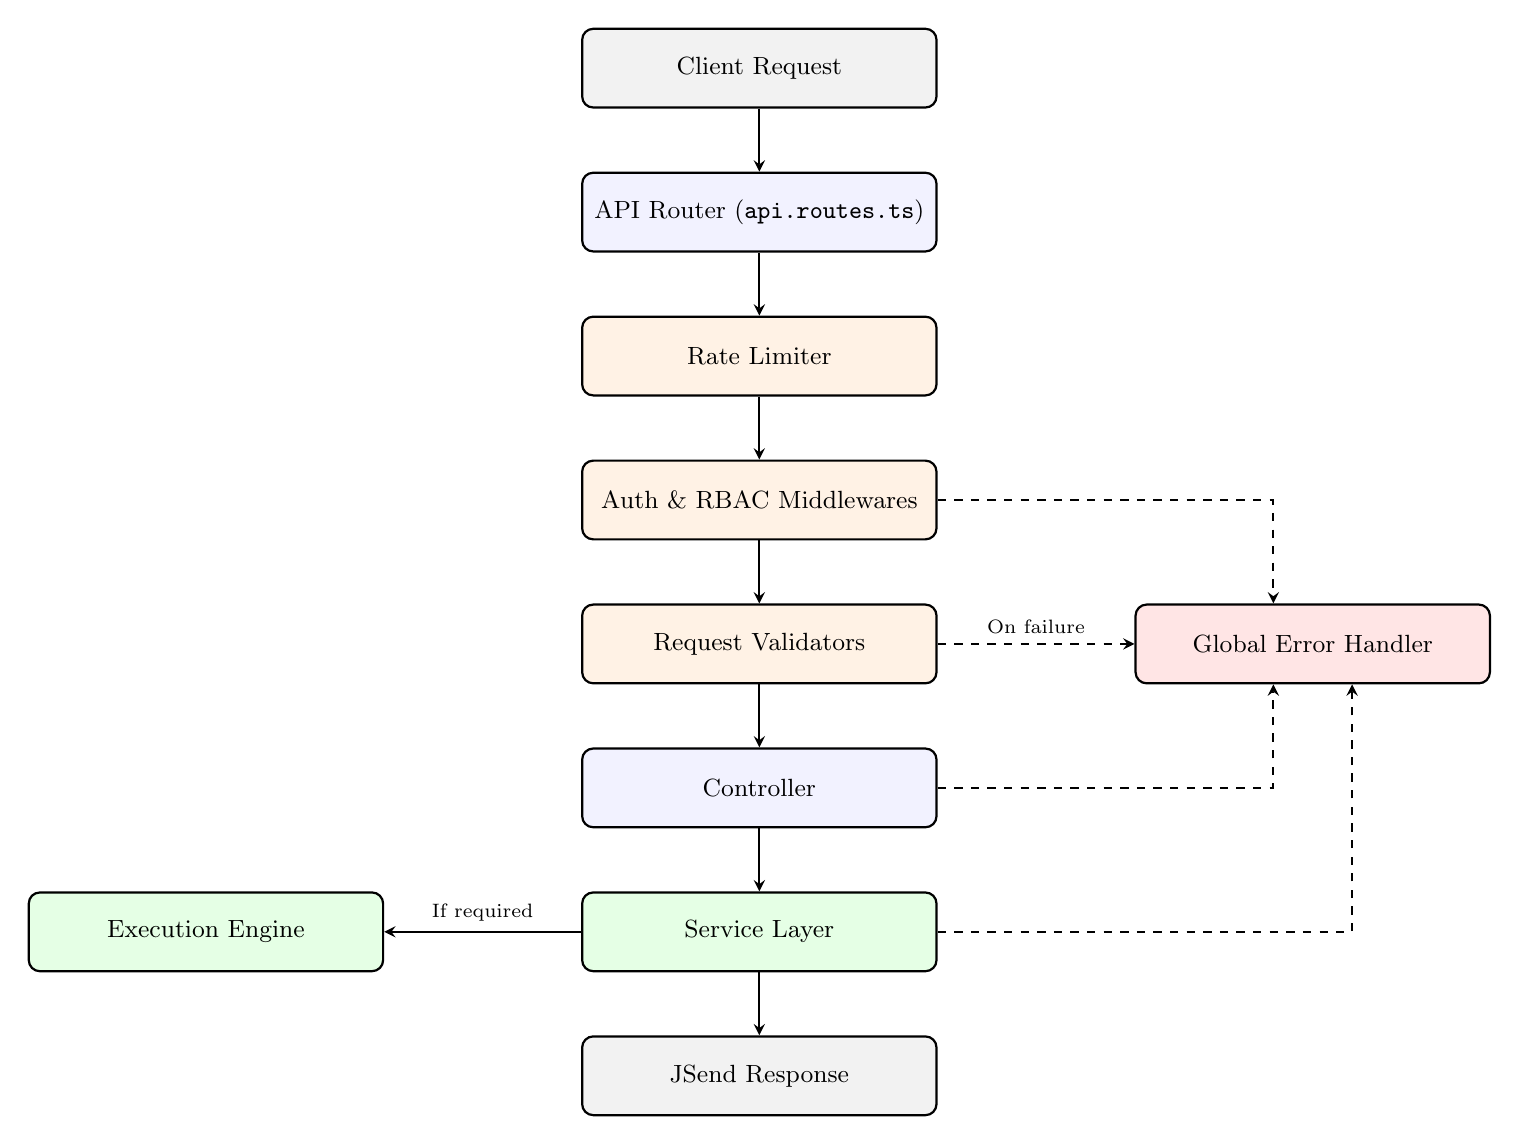
\begin{tikzpicture}[
  node distance=0.8cm and 2.5cm,
  box/.style={rectangle, draw=black, fill=blue!5, thick, minimum width=4.5cm, minimum height=1cm, text centered, rounded corners, font=\small},
  middleware/.style={rectangle, draw=black, fill=orange!10, thick, minimum width=4.5cm, minimum height=1cm, text centered, rounded corners, font=\small},
  logic/.style={rectangle, draw=black, fill=green!10, thick, minimum width=4.5cm, minimum height=1cm, text centered, rounded corners, font=\small},
  arrow/.style={thick, ->, >=stealth},
  dashed_arrow/.style={thick, ->, >=stealth, dashed}
]

% Main vertical pipeline
\node (client) [box, fill=gray!10] {Client Request};
\node (router) [box, below=of client] {API Router (\texttt{api.routes.ts})};
\node (rate) [middleware, below=of router] {Rate Limiter};
\node (auth) [middleware, below=of rate] {Auth \& RBAC Middlewares};
\node (validator) [middleware, below=of auth] {Request Validators};
\node (controller) [box, below=of validator] {Controller};
\node (service) [logic, below=of controller] {Service Layer};
\node (response) [box, fill=gray!10, below=of service] {JSend Response};

% Side nodes
\node (execution) [logic, left=of service] {Execution Engine};
\node (error) [middleware, fill=red!10, right=of validator] {Global Error Handler};

% Solid arrows (main flow)
\draw [arrow] (client) -- (router);
\draw [arrow] (router) -- (rate);
\draw [arrow] (rate) -- (auth);
\draw [arrow] (auth) -- (validator);
\draw [arrow] (validator) -- (controller);
\draw [arrow] (controller) -- (service);
\draw [arrow] (service) -- (response);
\draw [arrow] (service) -- (execution) node[midway, above, font=\scriptsize] {If required};

% Dashed arrows (Error handling) - routed cleanly to avoid overlapping
\draw [dashed_arrow] (auth.east) -| ([xshift=-0.5cm]error.north);
\draw [dashed_arrow] (validator.east) -- (error.west) node[midway, above, font=\scriptsize] {On failure};
\draw [dashed_arrow] (controller.east) -| ([xshift=-0.5cm]error.south);
\draw [dashed_arrow] (service.east) -| ([xshift=0.5cm]error.south);

\end{tikzpicture}
} % <--- Closed the resizebox here
\caption{High-level lifecycle of an incoming API request}
\label{fig:request-flow}
\end{figure}

\subsection{Backend System Layers}

The directory structure directly reflects the architectural boundaries of the application. Each layer has a single, distinct responsibility.

\subsubsection{Routes}
The routing layer is responsible for mapping incoming HTTP endpoints to their corresponding controller handlers. It acts as the entry point for the API hierarchy. Routes are logically grouped by entity (e.g., users, projects, workflows, nodes) and define the specific middleware chain required for each endpoint. 

By keeping the routing layer declarative, it provides a clear, high-level map of the entire API surface without bleeding into implementation details.

\subsubsection{Middlewares}
Middlewares act as the gatekeepers of the application. They intercept incoming requests to enforce systemic rules before the request can reach the business logic. This layer handles security concerns such as JSON Web Token (JWT) verification, role-based access control (RBAC), and email verification checks.

Additionally, middlewares manage traffic control via strict rate limiters, standardize outgoing success responses using the JSend format, and intercept exceptions through a centralized, registry-based error handling mechanism.

\subsubsection{Validators}
Request validation is abstracted into its own layer using \texttt{express-validator}. Before a request payload is processed, it is checked against strict schemas to ensure data integrity and type safety.

This layer ensures that bad payloads, missing parameters, or malformed data are rejected immediately with a \texttt{422 Unprocessable Entity} response. This "fail-fast" approach guarantees that the underlying controllers and services do not need to perform redundant sanity checks on incoming data.

\subsubsection{Controllers}
Controllers serve strictly as orchestrators between the HTTP transport layer and the business logic. A controller's only responsibility is to extract data from the incoming request (headers, body, params, query), pass that data to the appropriate service, and return the service's output back to the client.

Controllers are intentionally kept thin; they do not contain complex business rules or database queries, adhering strictly to the Single Responsibility Principle.

\subsubsection{Services}
The service layer forms the heart of the backend, encapsulating the core business logic of the FLOO platform. All heavy lifting—such as workflow graph construction, file processing with Cloudinary, communicating with the LLM via Groq, and interacting with the database—happens here.

By isolating business logic into services, the code becomes highly reusable and independently testable. For example, the execution engine can invoke a service method directly without needing to mock an HTTP request.

\subsubsection{Strategies}
The strategies layer encapsulates interchangeable authentication algorithms and behaviors, specifically leveraging Passport.js for OAuth 2.0 integrations. 

This directory contains the logic required to negotiate with external identity providers (such as Google, GitHub, and Discord) and third-party APIs like Google Sheets. Separating these into strategies allows the platform to easily scale the number of supported integrations without cluttering the core authentication flow.

\subsubsection{Utils}
The utils directory houses pure, stateless helper functions that are shared across multiple layers of the application. These include cryptographic operations like hashing passwords with \texttt{bcryptjs}, generating JWTs, and creating one-time passwords (OTPs) for email verification. 

Because these functions are pure and self-contained, they are highly reliable and prevent code duplication throughout the codebase.

\subsubsection{Types}
TypeScript interfaces and type definitions form the foundational contract of the application. The types layer defines the exact shape of data structures used across the system, such as augmented Express Request objects (\texttt{AuthRequest}) or standardized OAuth profiles. 

This layer ensures strict compile-time safety, allowing the compiler to catch structural mismatches between the frontend payloads, the internal API representation, and the execution engine.


\section{Data Layer Architecture}

\subsection{Database Requirements}
The FLOO platform requires a robust, relational data storage layer capable of supporting multi-tenant isolation, complex configuration storage, and strict security compliance. The primary storage needs encompass:
\begin{itemize}
    \item \textbf{User and Identity Management:} Tracking local user profiles, multi-provider OAuth identities, and RBAC roles to ensure secure, isolated workspaces.
    \item \textbf{Project and Workflow Configurations:} Storing dynamic, graph-based automation logic and tracking deployment states.
    \item \textbf{Execution Analytics:} Persisting detailed logs of workflow runs, statuses, and generated outputs (such as Cloudinary asset links) for debugging and system analytics.
    \item \textbf{Secure Credential Management:} Safely storing third-party integration secrets (e.g., API keys, OAuth tokens) utilizing an encrypted, dynamically generated structure.
\end{itemize}

\textbf{Key Drivers:} Relational integrity is paramount due to the highly interconnected nature of the platform. For example, a User owns Projects, which trigger Executions, which in turn generate NodeOutputs. Transactional safety is explicitly required for operations like cascading account deletions, ensuring that scrubbing a user removes all associated relational assets without creating orphaned records. Prisma was selected as the ORM to enforce these strict foreign key constraints while providing end-to-end type safety with the TypeScript backend.

\subsection{Conceptual Design (ERD)}
The Conceptual Entity Relationship Diagram (CERD) outlines the high-level business entities and their interactions.

%\begin{figure}[H]
%    \centering
 %   \includegraphics[width=\textwidth]{CERD.drawio.jpg}
  %  \caption{Conceptual Entity Relationship Diagram (CERD) for the FLOO platform \href{https://drive.google.com/file/d/1w0RLbndet0nz7lhRF8SNmPFbpWwuH5Ox/view}{[Source]}}
 %   \label{fig:cerd}
%\end{figure}

\subsubsection{Core Entity Relationships}
The conceptual model is heavily centered around the \texttt{User} entity, enforcing a strict ownership hierarchy:
\begin{itemize}
    \item \textbf{Users to Projects (1:N):} A single user can create and manage multiple automation projects. All workflow executions, chat histories, and node interactions branch off this fundamental relationship.
    \item \textbf{Projects to Executions (1:N):} Every time a workflow is triggered, an execution record is generated to track its lifecycle (e.g., NEW, RUNNING, SUCCESS, ERROR).
    \item \textbf{Nodes to Files (1:N):} External files are represented conceptually as inputs and outputs bound to specific execution instances and nodes, tracking cloud storage references.
\end{itemize}

\subsubsection{The Dynamic Credential Architecture}
A major architectural redesign was implemented in the credentials subsystem to provide a deep, highly flexible solution that seamlessly bridges backend storage with dynamic frontend UI rendering. 

Instead of hardcoding specific integration tokens into a single table, the system abstracts credentials into a definition-and-value pattern:
\begin{itemize}
    \item \textbf{Definition Phase:} Admins define a \texttt{CredentialType} (e.g., "Google Sheets" or "SMTP"). This type has a 1:N relationship with \texttt{CredentialParameterType}, which outlines the specific fields required (e.g., "API Key", "Client Secret").
    \item \textbf{UI Control Integration:} The \texttt{CredentialParameterType} includes metadata fields like \texttt{maxChar} and \texttt{isSensitive}. This design allows the frontend UI to automatically generate forms with appropriate validation and hidden password inputs without hardcoding frontend logic for every new integration type.
    \item \textbf{Value Phase:} When a user connects an integration, the system generates a \texttt{UserCredentialSet} linking to the \texttt{CredentialType}. The actual encrypted secrets are stored in \texttt{UserCredentialValue} records, creating a normalized mapping back to the expected parameters.
\end{itemize}

\subsection{Mapping to Relational Model (Logical/Physical Design)}
The logical design translates the conceptual entities into concrete database tables, explicitly defining keys, data types, and constraints utilizing the Prisma schema.

%\begin{figure}[H]
 %   \centering

 %   \includegraphics[width=\textwidth]{PERD.drawio.jpg}
%    \caption{Physical Entity Relationship Diagram (PERD) mapped to PostgreSQL}
%    \label{fig:perd}
%\end{figure}

\subsubsection{Primary and Foreign Key Strategy}
\begin{itemize}
    \item \textbf{Universal UUIDs:} All primary keys (PK) across the platform utilize auto-generated UUIDs (e.g., \texttt{@id @default(uuid())}). This strategy prevents resource enumeration attacks and ensures global uniqueness, particularly useful when merging distributed data.
    \item \textbf{Composite Constraints:} Certain tables utilize composite keys to enforce logical uniqueness. For example, \texttt{AuthIdentityProvider} uses \texttt{@@id([provider, providerId])} to ensure a user cannot link the same third-party account twice. Similarly, \texttt{UserCredentialValue} enforces \texttt{@@unique([setId, paramId])} to guarantee only one value exists per parameter in a given credential set.
    \item \textbf{Aggressive Cascading Deletions:} To maintain strict data hygiene and comply with PII scrubbing requirements, foreign keys aggressively employ \texttt{onDelete: Cascade}. Deleting a User cascades down to erase their Projects, which in turn wipes Executions, Node Inputs, and Chat Messages instantly at the database level.
\end{itemize}

\subsubsection{Junction and Mapping Tables}
The database features specific mapping tables to resolve complex relationships. \texttt{UserCredentialValue} serves as the critical junction between a user's \texttt{UserCredentialSet} and the system's \texttt{CredentialParameterType}. This normalized approach ensures that if a parameter requirement changes at the system level, the relationship to the user's stored values remains structurally intact.

\subsubsection{Intentional Denormalization (JSON Workflows)}
While the database is heavily normalized, a deliberate exception was made for workflow graph configurations. Rather than splitting workflow nodes, edges, and positions into dozens of relational tables, the entire graph is serialized and stored in a \texttt{Json} column within the \texttt{Project} table (\texttt{workflow Json?}). 

This is a strategic design choice: workflow graphs are exclusively read and updated as a single atomic unit by the React Flow frontend. Normalizing the graph would require complex, expensive recursive SQL joins upon every canvas load. Utilizing a JSON column provides the necessary schema flexibility for varied node data while preserving high-performance read/write operations.

\subsection{Physical Database Design \& Implementation}

The physical database layer is implemented using PostgreSQL hosted on Supabase. We utilize Prisma ORM to enforce end-to-end type safety across the application. The schema is maintained through declarative migrations, ensuring that the database state is always synchronized with our TypeScript interfaces. Sensitive data, such as integration credentials, is stored using standard text fields, with robust encryption and decryption logic handled strictly at the Service Layer before ever reaching the persistence layer.

\subsubsection{Database Engine: PostgreSQL (via Supabase)}
PostgreSQL was selected as the underlying engine for its strict adherence to ACID compliance, robust support for relational integrity, and advanced JSON processing capabilities. Hosting via Supabase provides managed scaling, automated backups, and connection pooling, ensuring the database can handle high-frequency reads and writes typical of an automated workflow engine.

\subsubsection{ORM Layer (Prisma)}
Prisma acts as the bridge between the Node.js backend and the PostgreSQL database. Rather than writing raw SQL queries, the application relies on the generated Prisma Client.
\begin{itemize}
    \item \textbf{Type Safety:} The `schema.prisma` file serves as the single source of truth. Changes to the schema automatically regenerate TypeScript definitions, ensuring that any mismatched queries, missing fields, or incorrect data types are caught at compile-time rather than throwing unexpected runtime errors.
    \item \textbf{JSON Workflows:} Prisma natively supports PostgreSQL's `JSONB` data type, allowing the `Project` table to store complex, nested React Flow graphs in the `workflow` column without sacrificing query performance or requiring excessive normalization.
\end{itemize}

\subsubsection{Migration Management}
Database schema evolution is managed via Prisma Migrations. Instead of executing manual SQL scripts directly against production, developers modify the declarative Prisma schema. The migration engine then generates deterministic SQL differential scripts. This approach ensures that schema changes are strictly version-controlled, reproducible across local, staging, and production environments, and seamlessly integrated into the CI/CD pipeline.

\subsubsection{Technical Constraints}
To guarantee data integrity and query performance at scale, several constraints are baked directly into the physical schema:

\paragraph{Indexes}
Indexes are strategically applied to fields that are frequently used in `WHERE` clauses, sorting operations, or foreign key lookups to prevent full table scans:
\begin{itemize}
    \item \textbf{Foreign Key Lookups:} Indexes on `userId` within the `Project` and `NodeInput` tables drastically reduce query times when an authenticated user requests their dashboard.
    \item \textbf{Lookup Optimization:} The `email` column in the `User` table is indexed to optimize the high-frequency login and registration authentication flows.
    \item \textbf{Composite Indexes:} High-traffic logging tables utilize composite indexes, such as `@@index([executionId, nodeId])` on `NodeOutput`, enabling rapid retrieval of execution assets for the frontend analytics UI.
\end{itemize}

\paragraph{Constraints}
\begin{itemize}
    \item \textbf{Primary Keys:} All entities utilize UUIDs (`@id @default(uuid())`) as primary keys. This prevents resource enumeration attacks (e.g., guessing a user's ID) and facilitates distributed data merging.
    \item \textbf{Unique Constraints:} `@@unique` constraints enforce strict data uniqueness, such as ensuring no two users share an `email`, and no two files share a Cloudinary `publicId`.
    \item \textbf{Composite Uniques:} The `UserCredentialValue` table employs `@@unique([setId, paramId])` to guarantee that a specific credential set contains exactly one value per required parameter, preventing duplicate secret injection.
\end{itemize}

\paragraph{Cascade Rules \& Account Deletion}
Foreign key cascading is aggressively utilized to enforce data hygiene and simplify backend logic. In the schema, relations defining ownership are marked with `onDelete: Cascade`. 

This is highly crucial for the platform's \textbf{Account Deletion Flow}. When a user self-deletes (or is purged by an admin), the database engine natively and atomically destroys all linked `Project` rows. The cascade continues downward, automatically erasing all `Execution` logs, `NodeInput` assets, and `UserCredentialSet` secrets. This guarantees compliance with PII scrubbing requirements without requiring the application service layer to manually fetch and delete thousands of related rows, effectively preventing orphaned data.

% ---------------------------------------------------------

\subsection{Data Dictionary}
The following tables detail the physical layout, constraints, and definitions of the core entities in the FLOO system.

\subsubsection{User Table}
Serves as the root entity for identity, access control, and ownership.
\begin{table}[H]
\centering
\renewcommand{\arraystretch}{1.3}
\begin{tabularx}{\textwidth}{|l|l|l|X|}
\hline
\textbf{Column Name} & \textbf{Type} & \textbf{Constraints} & \textbf{Description} \\
\hline
\texttt{id} & UUID & PK & Unique identifier for the user. \\
\hline
\texttt{email} & VARCHAR & Unique, Index & The user's primary email address for authentication. \\
\hline
\texttt{password} & VARCHAR & Nullable & Bcrypt-hashed local password. Null if using strictly OAuth. \\
\hline
\texttt{isVerified} & BOOLEAN & Default: false & Gates access to execution features until email is confirmed. \\
\hline
\texttt{role} & ENUM & Default: USER & Defines RBAC privileges (USER or ADMIN). \\
\hline
\end{tabularx}
\caption{Data Dictionary: User Table}
\label{tab:dict-user}
\end{table}

\subsubsection{Project Table}
Stores the configuration and state of the user's workflow automations.
\begin{table}[H]
\centering
\renewcommand{\arraystretch}{1.3}
\begin{tabularx}{\textwidth}{|l|l|l|X|}
\hline
\textbf{Column Name} & \textbf{Type} & \textbf{Constraints} & \textbf{Description} \\
\hline
\texttt{id} & UUID & PK & Unique identifier for the project. \\
\hline
\texttt{userId} & UUID & FK, Cascade & References \texttt{User.id}. Defines ownership. \\
\hline
\texttt{name} & VARCHAR & Not Null & Human-readable name of the automation. \\
\hline
\texttt{workflow} & JSONB & Nullable & Serialized React Flow graph containing node and edge definitions. \\
\hline
\texttt{deployed} & BOOLEAN & Default: false & Tracks whether the project is actively running trigger nodes. \\
\hline
\end{tabularx}
\caption{Data Dictionary: Project Table}
\label{tab:dict-project}
\end{table}

\subsubsection{UserCredentialSet Table}
Acts as the parent entity for a group of encrypted third-party integration secrets.
\begin{table}[H]
\centering
\renewcommand{\arraystretch}{1.3}
\begin{tabularx}{\textwidth}{|l|l|l|X|}
\hline
\textbf{Column Name} & \textbf{Type} & \textbf{Constraints} & \textbf{Description} \\
\hline
\texttt{id} & UUID & PK & Unique identifier for the credential set. \\
\hline
\texttt{userId} & UUID & FK, Cascade & References \texttt{User.id}. Determines who can use these credentials. \\
\hline
\texttt{typeId} & UUID & FK, Cascade & References \texttt{CredentialType.id} (e.g., Google Sheets, SMTP). \\
\hline
\texttt{label} & VARCHAR & Not Null & User-defined alias for the credentials (e.g., "My Work Gmail"). \\
\hline
\end{tabularx}
\caption{Data Dictionary: UserCredentialSet Table}
\label{tab:dict-credentialset}
\end{table}

\subsubsection{Execution Table}
Persists the lifecycle state and telemetry data for individual workflow runs.
\begin{table}[H]
\centering
\renewcommand{\arraystretch}{1.3}
\begin{tabularx}{\textwidth}{|l|l|l|X|}
\hline
\textbf{Column Name} & \textbf{Type} & \textbf{Constraints} & \textbf{Description} \\
\hline
\texttt{id} & UUID & PK & Unique tracking identifier for the job. \\
\hline
\texttt{projectId} & UUID & FK, Cascade & References \texttt{Project.id}. The workflow that was triggered. \\
\hline
\texttt{status} & ENUM & Default: NEW & Tracks the current state (NEW, RUNNING, SUCCESS, ERROR). \\
\hline
\texttt{error} & TEXT & Nullable & Stores execution stack traces or API failure messages if the run crashed. \\
\hline
\texttt{startedAt} & TIMESTAMP & Nullable & The exact time the execution engine picked up the job. \\
\hline
\end{tabularx}
\caption{Data Dictionary: Execution Table}
\label{tab:dict-execution}
\end{table}







% ─────────────────────────────────────────────
\section{API \& Application Layer}
\subsection{API Overview}

The FLOO platform is built on a modular, multi-layered architecture using Node.js, Express.js, and TypeScript, designed to ensure a strict separation of concerns between routing, business logic, security, and execution.

\subsubsection{RESTful Conventions}
The API is designed around RESTful principles, where resources are mapped to intuitive endpoints categorized by entity (e.g., \texttt{/user}, \texttt{/project}, \texttt{/node}, \texttt{/credential}). By maintaining a declarative routing structure, the API surface remains clean and self-documenting, preventing business logic from bleeding into the transport layer. The platform utilizes standard HTTP verbs to perform operations:
\begin{itemize}
    \item \textbf{GET}: Retrieve data or list resources.
    \item \textbf{POST}: Create new resources or trigger actions.
    \item \textbf{PATCH}: Update existing resource metadata.
    \item \textbf{DELETE}: Remove specific resources or clear session data.
\end{itemize}

\subsubsection{Authentication and Security}
Security is enforced through a tiered middleware system that acts as the application's gatekeeper.
\begin{itemize}
    \item \textbf{JWT Authentication}: Most endpoints require a valid JSON Web Token (JWT) processed by the \texttt{auth} middleware to identify the requesting user.
    \item \textbf{Role-Based Access Control (RBAC)}: Sensitive routes utilize the \texttt{restrictTo} middleware to enforce fine-grained access based on user roles (\texttt{USER} vs \texttt{ADMIN}).
    \item \textbf{Verification Gate}: Critical operations, such as managing projects or executing workflows, are protected by the \texttt{restrictToVerified} middleware, ensuring only accounts with confirmed emails can perform these actions.
    \item \textbf{Public Access}: Certain endpoints, such as initial Auth/OAuth routes and Webhook triggers, allow public access. These are not left unprotected but are instead secured via dedicated, high-threshold rate limiters.
\end{itemize}

\subsubsection{Response Format and Standardization}
To ensure consistency across the platform, all responses adhere to the \textbf{JSend} format, providing a predictable structure for the frontend.

\paragraph{HTTP Status Codes}
The API utilizes standard HTTP status codes to communicate outcome states:
\begin{table}[H]
\centering
\begin{tabular}{|l|p{8cm}|}
\hline
\textbf{Code} & \textbf{Meaning} \\
\hline
\texttt{200/201} & Successful request or creation. \\
\hline
\texttt{400} & Bad Request (Missing fields, validation failure). \\
\hline
\texttt{401} & Authentication failed (Expired or invalid token). \\
\hline
\texttt{403} & Forbidden (Insufficient permissions or unverified email). \\
\hline
\texttt{404} & Resource not found. \\
\hline
\texttt{429} & Too Many Requests (Rate limit exceeded). \\
\hline
\texttt{500} & Internal Server Error (Unexpected system failure). \\
\hline
\end{tabular}
\end{table}

\paragraph{Rate Limiting}
Traffic control is central to platform stability. The system employs multiple tiers of rate limiting:
\begin{itemize}
    \item \textbf{Standard Limit}: Most API routes are subject to a global limit of 150 requests per 15 minutes to prevent abuse.
    \item \textbf{Action-Specific Limits}: Critical actions have stricter, dedicated limits—such as manual workflow execution (30/min), file uploads (20/15min), or OAuth requests (10/15min)—to protect high-cost resources.
    \item \textbf{Public Limits}: High-volume triggers, like webhooks, utilize a loose limit (e.g., 1000/min) to accommodate frequent event spikes from external providers.
\end{itemize}

\subsection{Endpoints Reference}
\subsubsection{Auth Endpoints}
\label{subsec:auth-endpoints}

This section documents all API endpoints related to user authentication, registration, and session management in FLOO. Most of these endpoints are public but are protected by strict rate limiters and payload validators (\texttt{validateRequest}) to ensure security and prevent abuse.

% ─────────────────────────────────────────────
\paragraph{Register User}
\label{subsubsec:register-user}

\begin{itemize}
  \item \textbf{Endpoint:} \texttt{POST /api/auth/register}
  \item \textbf{Access:} \texttt{PUBLIC}
  \item \textbf{Description:} Creates a new user account and sends a verification code (OTP) to the provided email. Rate limited to 3 requests per hour per IP.
\end{itemize}

\begin{table}[H]
\centering
\renewcommand{\arraystretch}{1.3}
\begin{tabularx}{\textwidth}{|l|l|l|X|}
\hline
\textbf{Field} & \textbf{Location} & \textbf{Type} & \textbf{Description} \\
\hline
\texttt{email}     & Body & \texttt{string} & \textbf{Required.} User's email address \\
\hline
\texttt{password}  & Body & \texttt{string} & \textbf{Required.} User's password \\
\hline
\texttt{firstName} & Body & \texttt{string} & \textbf{Required.} User's first name \\
\hline
\texttt{lastName}  & Body & \texttt{string} & \textbf{Required.} User's last name \\
\hline
\end{tabularx}
\caption{POST /api/auth/register — Request Body}
\label{tab:register-body}
\end{table}

\begin{table}[H]
\centering
\renewcommand{\arraystretch}{1.3}
\begin{tabularx}{\textwidth}{|l|l|X|}
\hline
\textbf{Status Code} & \textbf{Condition} & \textbf{Description} \\
\hline
\texttt{201 Created}      & Success            & Verification code sent, returns user and tokens \\
\hline
\texttt{409 Conflict}     & Email in use       & A user with this email already exists \\
\hline
\texttt{422 Unprocessable Entity} & Validation failed & Required fields missing or invalid \\
\hline
\texttt{429 Too Many Requests} & Rate limit exceeded & Too many accounts created from this IP, please try again after an hour \\
\hline
\texttt{500 Internal Server Error} & Server error & Unexpected failure or email delivery issue \\
\hline
\end{tabularx}
\caption{POST /api/auth/register — Response Codes}
\label{tab:register-responses}
\end{table}
\FloatBarrier

% ─────────────────────────────────────────────
\paragraph{Login User}
\label{subsubsec:login-user}

\begin{itemize}
  \item \textbf{Endpoint:} \texttt{POST /api/auth/login}
  \item \textbf{Access:} \texttt{PUBLIC}
  \item \textbf{Description:} Authenticates a user using email and password. Cannot be used for accounts created exclusively via OAuth. Rate limited to 5 attempts per 15 minutes per IP.
\end{itemize}

\begin{table}[H]
\centering
\renewcommand{\arraystretch}{1.3}
\begin{tabularx}{\textwidth}{|l|l|l|X|}
\hline
\textbf{Field} & \textbf{Location} & \textbf{Type} & \textbf{Description} \\
\hline
\texttt{email}    & Body & \texttt{string} & \textbf{Required.} The user's email \\
\hline
\texttt{password} & Body & \texttt{string} & \textbf{Required.} The user's password \\
\hline
\end{tabularx}
\caption{POST /api/auth/login — Request Body}
\label{tab:login-body}
\end{table}

\begin{table}[H]
\centering
\renewcommand{\arraystretch}{1.3}
\begin{tabularx}{\textwidth}{|l|l|X|}
\hline
\textbf{Status Code} & \textbf{Condition} & \textbf{Description} \\
\hline
\texttt{200 OK}           & Success            & Returns user data, access token, and refresh token \\
\hline
\texttt{401 Unauthorized} & Invalid credentials & Wrong email, password, or OAuth-only account \\
\hline
\texttt{422 Unprocessable Entity} & Validation failed & Required fields missing or invalid \\
\hline
\texttt{429 Too Many Requests} & Rate limit exceeded & Too many login attempts from this IP, please try again after 15 minutes \\
\hline
\texttt{500 Internal Server Error} & Server error & Unexpected failure \\
\hline
\end{tabularx}
\caption{POST /api/auth/login — Response Codes}
\label{tab:login-responses}
\end{table}
\FloatBarrier

% ─────────────────────────────────────────────
\paragraph{Forgot Password}
\label{subsubsec:forgot-password}

\begin{itemize}
  \item \textbf{Endpoint:} \texttt{POST /api/auth/forgot-password}
  \item \textbf{Access:} \texttt{PUBLIC}
  \item \textbf{Description:} Generates a 15-minute OTP and sends it to the user's email to reset their password. Always returns a success message for security reasons, even if the email is unregistered. Rate limited to 3 requests per hour.
\end{itemize}

\begin{table}[H]
\centering
\renewcommand{\arraystretch}{1.3}
\begin{tabularx}{\textwidth}{|l|l|l|X|}
\hline
\textbf{Field} & \textbf{Location} & \textbf{Type} & \textbf{Description} \\
\hline
\texttt{email} & Body & \texttt{string} & \textbf{Required.} The account email address \\
\hline
\end{tabularx}
\caption{POST /api/auth/forgot-password — Request Body}
\label{tab:forgot-password-body}
\end{table}

\begin{table}[H]
\centering
\renewcommand{\arraystretch}{1.3}
\begin{tabularx}{\textwidth}{|l|l|X|}
\hline
\textbf{Status Code} & \textbf{Condition} & \textbf{Description} \\
\hline
\texttt{200 OK}           & Success            & Reset code sent successfully \\
\hline
\texttt{422 Unprocessable Entity} & Validation failed & Invalid email format \\
\hline
\texttt{429 Too Many Requests} & Rate limit exceeded & Too many password reset requests, please try again after an hour \\
\hline
\texttt{500 Internal Server Error} & Server error & Unexpected failure or email delivery issue \\
\hline
\end{tabularx}
\caption{POST /api/auth/forgot-password — Response Codes}
\label{tab:forgot-password-responses}
\end{table}
\FloatBarrier

% ─────────────────────────────────────────────
\paragraph{Verify Reset Code (Reset Password)}
\label{subsubsec:reset-password}

\begin{itemize}
  \item \textbf{Endpoint:} \texttt{POST /api/auth/reset-password}
  \item \textbf{Access:} \texttt{PUBLIC}
  \item \textbf{Description:} Validates the OTP sent via email and updates the user's password. The new password cannot match the old password. Rate limited to 3 requests per hour.
\end{itemize}

\begin{table}[H]
\centering
\renewcommand{\arraystretch}{1.3}
\begin{tabularx}{\textwidth}{|l|l|l|X|}
\hline
\textbf{Field} & \textbf{Location} & \textbf{Type} & \textbf{Description} \\
\hline
\texttt{email}     & Body & \texttt{string} & \textbf{Required.} The account email \\
\hline
\texttt{resetCode} & Body & \texttt{string} & \textbf{Required.} The OTP sent to the user \\
\hline
\texttt{password}  & Body & \texttt{string} & \textbf{Required.} The new password \\
\hline
\end{tabularx}
\caption{POST /api/auth/reset-password — Request Body}
\label{tab:reset-password-body}
\end{table}

\begin{table}[H]
\centering
\renewcommand{\arraystretch}{1.3}
\begin{tabularx}{\textwidth}{|l|l|X|}
\hline
\textbf{Status Code} & \textbf{Condition} & \textbf{Description} \\
\hline
\texttt{200 OK}           & Success             & Password reset successfully \\
\hline
\texttt{400 Bad Request}  & Invalid code        & The OTP is incorrect or expired \\
\hline
\texttt{401 Unauthorized} & Same password       & The new password is the same as the old one \\
\hline
\texttt{422 Unprocessable Entity} & Validation failed & Missing fields or invalid format \\
\hline
\texttt{429 Too Many Requests} & Rate limit exceeded & Too many password reset requests, please try again after an hour \\
\hline
\texttt{500 Internal Server Error} & Server error & Unexpected failure \\
\hline
\end{tabularx}
\caption{POST /api/auth/reset-password — Response Codes}
\label{tab:reset-password-responses}
\end{table}
\FloatBarrier

% ─────────────────────────────────────────────
\paragraph{Refresh Token}
\label{subsubsec:refresh-token}

\begin{itemize}
  \item \textbf{Endpoint:} \texttt{POST /api/auth/refresh-token}
  \item \textbf{Access:} \texttt{PUBLIC}
  \item \textbf{Description:} Exchanges a valid refresh token for a new access token. Validates against the hashed token stored in the database. Rate limited to 5 requests per 15 minutes.
\end{itemize}

\begin{table}[H]
\centering
\renewcommand{\arraystretch}{1.3}
\begin{tabularx}{\textwidth}{|l|l|l|X|}
\hline
\textbf{Field} & \textbf{Location} & \textbf{Type} & \textbf{Description} \\
\hline
\texttt{refreshToken} & Body & \texttt{string} & \textbf{Required.} The user's active refresh token \\
\hline
\end{tabularx}
\caption{POST /api/auth/refresh-token — Request Body}
\label{tab:refresh-token-body}
\end{table}

\begin{table}[H]
\centering
\renewcommand{\arraystretch}{1.3}
\begin{tabularx}{\textwidth}{|l|l|X|}
\hline
\textbf{Status Code} & \textbf{Condition} & \textbf{Description} \\
\hline
\texttt{200 OK}           & Success              & Returns a new access token \\
\hline
\texttt{401 Unauthorized} & Invalid token        & Token is expired, missing in DB, or invalid \\
\hline
\texttt{429 Too Many Requests} & Rate limit exceeded & Too many token refresh requests from this IP \\
\hline
\texttt{500 Internal Server Error} & Server error & Unexpected failure \\
\hline
\end{tabularx}
\caption{POST /api/auth/refresh-token — Response Codes}
\label{tab:refresh-token-responses}
\end{table}
\FloatBarrier

% ─────────────────────────────────────────────
\paragraph{OAuth Initiation}
\label{subsubsec:oauth-initiation}

\begin{itemize}
  \item \textbf{Endpoints:} 
  \texttt{GET /api/auth/discord}, 
  \texttt{GET /api/auth/google}, 
  \texttt{GET /api/auth/github}
  \item \textbf{Access:} \texttt{PUBLIC}
  \item \textbf{Description:} Initiates the OAuth flow by redirecting the user to the respective provider's authentication page. Supports dynamic redirect configuration based on the client type. Rate limited to 10 requests per 15 minutes.
\end{itemize}

\begin{table}[H]
\centering
\renewcommand{\arraystretch}{1.3}
\begin{tabularx}{\textwidth}{|l|l|l|X|}
\hline
\textbf{Parameter} & \textbf{Location} & \textbf{Type} & \textbf{Description} \\
\hline
\texttt{client}    & Query & \texttt{string} & Optional. Pass \texttt{flutter} for mobile deep linking \\
\hline
\end{tabularx}
\caption{GET /api/auth/\{provider\} — Query Parameters}
\label{tab:oauth-initiation-params}
\end{table}

% ─────────────────────────────────────────────
\paragraph{OAuth Callback}
\label{subsubsec:oauth-callback}

\begin{itemize}
  \item \textbf{Endpoints:} 
  \texttt{GET /api/auth/discord/callback}, 
  \texttt{GET /api/auth/google/callback}, 
  \texttt{GET /api/auth/github/callback}
  \item \textbf{Access:} \texttt{PUBLIC}
  \item \textbf{Description:} Handled by Passport.js strategies. Upon successful authentication, it generates a secure 15-second ticket stored in Redis and redirects to the client application (Web or Flutter) with the ticket appended as a query parameter. Rate limited to 10 requests per 15 minutes.
\end{itemize}

\begin{table}[H]
\centering
\renewcommand{\arraystretch}{1.3}
\begin{tabularx}{\textwidth}{|l|l|X|}
\hline
\textbf{Status Code} & \textbf{Condition} & \textbf{Description} \\
\hline
\texttt{302 Found}        & Success            & Redirects to client URL with \texttt{?ticket=UUID} \\
\hline
\texttt{401 Unauthorized} & Auth failed        & Failed to login with the OAuth provider \\
\hline
\texttt{429 Too Many Requests} & Rate limit exceeded & Too many OAuth requests \\
\hline
\texttt{500 Internal Server Error} & Server error & Unexpected failure \\
\hline
\end{tabularx}
\caption{GET /api/auth/\{provider\}/callback — Response Codes}
\label{tab:oauth-callback-responses}
\end{table}
\FloatBarrier

% ─────────────────────────────────────────────
\paragraph{Exchange Ticket}
\label{subsubsec:exchange-ticket}

\begin{itemize}
  \item \textbf{Endpoint:} \texttt{POST /api/auth/exchange}
  \item \textbf{Access:} \texttt{PUBLIC}
  \item \textbf{Description:} Exchanges the temporary Redis ticket obtained from the OAuth callback for the actual user data, access token, and refresh token. The ticket is single-use and expires in 15 seconds. Rate limited to 10 requests per 15 minutes.
\end{itemize}

\begin{table}[H]
\centering
\renewcommand{\arraystretch}{1.3}
\begin{tabularx}{\textwidth}{|l|l|l|X|}
\hline
\textbf{Field} & \textbf{Location} & \textbf{Type} & \textbf{Description} \\
\hline
\texttt{ticket} & Body & \texttt{string} & \textbf{Required.} The UUID ticket from the OAuth redirect \\
\hline
\end{tabularx}
\caption{POST /api/auth/exchange — Request Body}
\label{tab:exchange-ticket-body}
\end{table}

\begin{table}[H]
\centering
\renewcommand{\arraystretch}{1.3}
\begin{tabularx}{\textwidth}{|l|l|X|}
\hline
\textbf{Status Code} & \textbf{Condition} & \textbf{Description} \\
\hline
\texttt{200 OK}           & Success              & Ticket exchanged, returns user and tokens \\
\hline
\texttt{400 Bad Request}  & Invalid ticket       & The ticket is invalid, expired, or already used \\
\hline
\texttt{422 Unprocessable Entity} & Validation failed & Missing ticket in request body \\
\hline
\texttt{429 Too Many Requests} & Rate limit exceeded & Too many OAuth requests \\
\hline
\texttt{500 Internal Server Error} & Server error & Unexpected failure \\
\hline
\end{tabularx}
\caption{POST /api/auth/exchange — Response Codes}
\label{tab:exchange-ticket-responses}
\end{table}
\clearpage
\FloatBarrier
\subsubsection{User Endpoints}
\label{subsec:user-endpoints}

This section documents all API endpoints related to user management, authentication profiles, and account controls in FLOO. Users and profiles are fundamental entities in the system. All endpoints in this section are protected by the \texttt{auth} middleware, requiring a valid JWT token. Role-based access control is strictly enforced via the \texttt{restricTo} middleware.

\textbf{Note on Verification and Rate Limiting:} Unlike project or execution routes, user routes can be accessed by authenticated accounts that are \textbf{not yet verified}, allowing them to manage their profile and complete the verification process. All user endpoints are subject to the standard API rate limit of 150 requests per 15 minutes, with stricter dedicated limiters applied to sensitive actions like email verification and password updates.

% ─────────────────────────────────────────────
\paragraph{Get All Users (Admin)}
\label{subsubsec:get-all-users}

\begin{itemize}
  \item \textbf{Endpoint:} \texttt{GET /api/user/all}
  \item \textbf{Access:} \texttt{ADMIN} only
  \item \textbf{Description:} Retrieves a paginated list of all users stored in the database. Supports dynamic filtering based on account status, roles, and partial text matches for personal details. Subject to the standard API rate limit.
\end{itemize}

\begin{table}[H]
\centering
\renewcommand{\arraystretch}{1.3}
\begin{tabularx}{\textwidth}{|l|l|l|X|}
\hline
\textbf{Parameter} & \textbf{Location} & \textbf{Type} & \textbf{Description} \\
\hline
\texttt{disabled}   & Query & \texttt{boolean} & Exact match filter for disabled status (\texttt{true}/\texttt{false}) \\
\hline
\texttt{isVerified} & Query & \texttt{boolean} & Exact match filter for verification status (\texttt{true}/\texttt{false}) \\
\hline
\texttt{role}       & Query & \texttt{string}  & Exact match for user role (e.g., \texttt{ADMIN}, \texttt{USER}) \\
\hline
\texttt{email}      & Query & \texttt{string}  & Case-insensitive partial match for email \\
\hline
\texttt{firstName}  & Query & \texttt{string}  & Case-insensitive partial match for first name \\
\hline
\texttt{lastName}   & Query & \texttt{string}  & Case-insensitive partial match for last name \\
\hline
\texttt{limit}      & Query & \texttt{integer} & Number of results to return (default: 100) \\
\hline
\texttt{skip}       & Query & \texttt{integer} & Number of results to skip for pagination (default: 0) \\
\hline
\end{tabularx}
\caption{GET /api/user/all — Query Parameters}
\label{tab:get-all-users-params}
\end{table}

\begin{table}[H]
\centering
\renewcommand{\arraystretch}{1.3}
\begin{tabularx}{\textwidth}{|l|l|X|}
\hline
\textbf{Status Code} & \textbf{Condition} & \textbf{Description} \\
\hline
\texttt{200 OK}           & Success      & Returns a paginated list of users \\
\hline
\texttt{401 Unauthorized} & No/invalid token & Authentication failed \\
\hline
\texttt{403 Forbidden}    & Non-admin user   & Insufficient permissions \\
\hline
\texttt{429 Too Many Requests} & Rate limit exceeded & Too many requests to the API \\
\hline
\texttt{500 Internal Server Error} & Server error & Unexpected failure \\
\hline
\end{tabularx}
\caption{GET /api/user/all — Response Codes}
\label{tab:get-all-users-responses}
\end{table}
\FloatBarrier

% ─────────────────────────────────────────────
\paragraph{Get User Profile}
\label{subsubsec:get-user-profile}

\begin{itemize}
  \item \textbf{Endpoint:} \texttt{GET /api/user/profile}
  \item \textbf{Access:} \texttt{USER}, \texttt{ADMIN}
  \item \textbf{Description:} Retrieves the authenticated user's own profile data. The user ID is automatically extracted from the JWT token. The profile must not be disabled. Subject to the standard API rate limit.
\end{itemize}

\begin{table}[H]
\centering
\renewcommand{\arraystretch}{1.3}
\begin{tabularx}{\textwidth}{|l|l|X|}
\hline
\textbf{Status Code} & \textbf{Condition} & \textbf{Description} \\
\hline
\texttt{200 OK}           & Success              & Returns the user's profile \\
\hline
\texttt{401 Unauthorized} & No/invalid token     & Authentication failed \\
\hline
\texttt{404 Not Found}    & Profile not found    & The user profile does not exist or is disabled \\
\hline
\texttt{429 Too Many Requests} & Rate limit exceeded & Too many requests to the API \\
\hline
\texttt{500 Internal Server Error} & Server error & Unexpected failure \\
\hline
\end{tabularx}
\caption{GET /api/user/profile — Response Codes}
\label{tab:get-user-profile-responses}
\end{table}
\FloatBarrier

% ─────────────────────────────────────────────
\paragraph{Get User by ID}
\label{subsubsec:get-user-by-id}

\begin{itemize}
  \item \textbf{Endpoint:} \texttt{GET /api/user/:id}
  \item \textbf{Access:} \texttt{ADMIN}, \texttt{USER}
  \item \textbf{Description:} Retrieves a specific user by their ID. Admins receive full details (including disabled accounts and sensitive fields), while standard users only see public-safe details of active accounts. Subject to the standard API rate limit.
\end{itemize}

\begin{table}[H]
\centering
\renewcommand{\arraystretch}{1.3}
\begin{tabularx}{\textwidth}{|l|l|l|X|}
\hline
\textbf{Parameter} & \textbf{Location} & \textbf{Type} & \textbf{Description} \\
\hline
\texttt{id} & URL & \texttt{string} & The target user's ID \\
\hline
\end{tabularx}
\caption{GET /api/user/:id — Parameters}
\label{tab:get-user-by-id-params}
\end{table}

\begin{table}[H]
\centering
\renewcommand{\arraystretch}{1.3}
\begin{tabularx}{\textwidth}{|l|l|X|}
\hline
\textbf{Status Code} & \textbf{Condition} & \textbf{Description} \\
\hline
\texttt{200 OK}           & Success              & Returns the user data (filtered based on requester role) \\
\hline
\texttt{400 Bad Request}  & Missing parameter    & User ID is required \\
\hline
\texttt{401 Unauthorized} & No/invalid token     & Authentication failed \\
\hline
\texttt{404 Not Found}    & User not found       & No user exists with the given ID (or is disabled for non-admins) \\
\hline
\texttt{429 Too Many Requests} & Rate limit exceeded & Too many requests to the API \\
\hline
\texttt{500 Internal Server Error} & Server error & Unexpected failure \\
\hline
\end{tabularx}
\caption{GET /api/user/:id — Response Codes}
\label{tab:get-user-by-id-responses}
\end{table}
\FloatBarrier

% ─────────────────────────────────────────────
\paragraph{Update My Profile}
\label{subsubsec:update-my-profile}

\begin{itemize}
  \item \textbf{Endpoint:} \texttt{PATCH /api/user/profile}
  \item \textbf{Access:} \texttt{USER}, \texttt{ADMIN}
  \item \textbf{Description:} Updates basic profile details for the authenticated user. At least one field must be provided. The request is validated before processing. Subject to the standard API rate limit.
\end{itemize}

\begin{table}[H]
\centering
\renewcommand{\arraystretch}{1.3}
\begin{tabularx}{\textwidth}{|l|l|l|X|}
\hline
\textbf{Field} & \textbf{Location} & \textbf{Type} & \textbf{Description} \\
\hline
\texttt{firstName}        & Body & \texttt{string}  & Optional. New first name \\
\hline
\texttt{lastName}         & Body & \texttt{string}  & Optional. New last name \\
\hline
\texttt{personalizations} & Body & \texttt{object}  & Optional. JSON object containing user personalizations \\
\hline
\end{tabularx}
\caption{PATCH /api/user/profile — Request Body}
\label{tab:update-my-profile-body}
\end{table}

\begin{table}[H]
\centering
\renewcommand{\arraystretch}{1.3}
\begin{tabularx}{\textwidth}{|l|l|X|}
\hline
\textbf{Status Code} & \textbf{Condition} & \textbf{Description} \\
\hline
\texttt{200 OK}           & Success              & Returns the updated user profile \\
\hline
\texttt{400 Bad Request}  & Empty body           & No fields provided to update \\
\hline
\texttt{401 Unauthorized} & No/invalid token     & Authentication failed \\
\hline
\texttt{404 Not Found}    & Profile not found    & User does not exist or is disabled \\
\hline
\texttt{422 Unprocessable Entity} & Validation failed & Invalid field values \\
\hline
\texttt{429 Too Many Requests} & Rate limit exceeded & Too many requests to the API \\
\hline
\texttt{500 Internal Server Error} & Server error & Unexpected failure \\
\hline
\end{tabularx}
\caption{PATCH /api/user/profile — Response Codes}
\label{tab:update-my-profile-responses}
\end{table}
\FloatBarrier

% ─────────────────────────────────────────────
\paragraph{Update My Email}
\label{subsubsec:update-my-email}

\begin{itemize}
  \item \textbf{Endpoint:} \texttt{PATCH /api/user/profile/email}
  \item \textbf{Access:} \texttt{USER}, \texttt{ADMIN}
  \item \textbf{Description:} Initiates an email change process. Updates the email, immediately revokes verification status, and sends a new OTP valid for 15 minutes. Also regenerates access and refresh tokens. Protected by a strict rate limiter to prevent email bombing (\textbf{3 requests per hour}).
\end{itemize}

\begin{table}[H]
\centering
\renewcommand{\arraystretch}{1.3}
\begin{tabularx}{\textwidth}{|l|l|l|X|}
\hline
\textbf{Field} & \textbf{Location} & \textbf{Type} & \textbf{Description} \\
\hline
\texttt{email} & Body & \texttt{string} & \textbf{Required.} The new email address \\
\hline
\end{tabularx}
\caption{PATCH /api/user/profile/email — Request Body}
\label{tab:update-my-email-body}
\end{table}

\begin{table}[H]
\centering
\renewcommand{\arraystretch}{1.3}
\begin{tabularx}{\textwidth}{|l|l|X|}
\hline
\textbf{Status Code} & \textbf{Condition} & \textbf{Description} \\
\hline
\texttt{200 OK}           & Success              & Email updated, code sent, and new tokens issued \\
\hline
\texttt{400 Bad Request}  & Identical email      & New email is identical to the current one \\
\hline
\texttt{401 Unauthorized} & No/invalid token     & Authentication failed \\
\hline
\texttt{404 Not Found}    & User not found       & User does not exist or is disabled \\
\hline
\texttt{409 Conflict}     & Email in use         & The requested email is already registered \\
\hline
\texttt{422 Unprocessable Entity} & Validation failed & Invalid email format \\
\hline
\texttt{429 Too Many Requests} & Rate limit exceeded & Too many verification emails sent (Max 3 per hour) \\
\hline
\texttt{500 Internal Server Error} & Server error & Unexpected failure \\
\hline
\end{tabularx}
\caption{PATCH /api/user/profile/email — Response Codes}
\label{tab:update-my-email-responses}
\end{table}
\FloatBarrier

% ─────────────────────────────────────────────
\paragraph{Update My Password}
\label{subsubsec:update-my-password}

\begin{itemize}
  \item \textbf{Endpoint:} \texttt{PATCH /api/user/profile/password}
  \item \textbf{Access:} \texttt{USER}, \texttt{ADMIN}
  \item \textbf{Description:} Updates the user's local password securely by verifying the old password first. Users authenticating via OAuth cannot use this route. Protected by a specific rate limiter to prevent brute force update attempts (\textbf{5 requests per hour}).
\end{itemize}

\begin{table}[H]
\centering
\renewcommand{\arraystretch}{1.3}
\begin{tabularx}{\textwidth}{|l|l|l|X|}
\hline
\textbf{Field} & \textbf{Location} & \textbf{Type} & \textbf{Description} \\
\hline
\texttt{oldPassword}     & Body & \texttt{string} & \textbf{Required.} The user's current password \\
\hline
\texttt{password}        & Body & \texttt{string} & \textbf{Required.} The new password \\
\hline
\texttt{confirmPassword} & Body & \texttt{string} & \textbf{Required.} Must match the new password \\
\hline
\end{tabularx}
\caption{PATCH /api/user/profile/password — Request Body}
\label{tab:update-my-password-body}
\end{table}

\begin{table}[H]
\centering
\renewcommand{\arraystretch}{1.3}
\begin{tabularx}{\textwidth}{|l|l|X|}
\hline
\textbf{Status Code} & \textbf{Condition} & \textbf{Description} \\
\hline
\texttt{200 OK}           & Success              & Password updated successfully \\
\hline
\texttt{400 Bad Request}  & Invalid update       & Passwords do not match, new is same as old, or OAuth user \\
\hline
\texttt{401 Unauthorized} & Authentication failed & Old password incorrect or token invalid \\
\hline
\texttt{404 Not Found}    & User not found       & User does not exist or is disabled \\
\hline
\texttt{422 Unprocessable Entity} & Validation failed & Password does not meet security requirements \\
\hline
\texttt{429 Too Many Requests} & Rate limit exceeded & Too many password update attempts (Max 5 per hour) \\
\hline
\texttt{500 Internal Server Error} & Server error & Unexpected failure \\
\hline
\end{tabularx}
\caption{PATCH /api/user/profile/password — Response Codes}
\label{tab:update-my-password-responses}
\end{table}
\FloatBarrier

% ─────────────────────────────────────────────
\paragraph{Update User Role (Admin)}
\label{subsubsec:update-user-role}

\begin{itemize}
  \item \textbf{Endpoint:} \texttt{PATCH /api/user/role/:id}
  \item \textbf{Access:} \texttt{ADMIN} only
  \item \textbf{Description:} Updates a specific user's role. Admins are explicitly prevented from changing their own role to avoid accidental or malicious demotions. Subject to the standard API rate limit.
\end{itemize}

\begin{table}[H]
\centering
\renewcommand{\arraystretch}{1.3}
\begin{tabularx}{\textwidth}{|l|l|l|X|}
\hline
\textbf{Field/Parameter} & \textbf{Location} & \textbf{Type} & \textbf{Description} \\
\hline
\texttt{id}   & URL  & \texttt{string} & \textbf{Required.} The target user's ID \\
\hline
\texttt{role} & Body & \texttt{string} & \textbf{Required.} The new role to assign \\
\hline
\end{tabularx}
\caption{PATCH /api/user/role/:id — Parameters}
\label{tab:update-user-role-params}
\end{table}

\begin{table}[H]
\centering
\renewcommand{\arraystretch}{1.3}
\begin{tabularx}{\textwidth}{|l|l|X|}
\hline
\textbf{Status Code} & \textbf{Condition} & \textbf{Description} \\
\hline
\texttt{200 OK}           & Success              & Returns the user with the updated role \\
\hline
\texttt{400 Bad Request}  & Missing role         & Role field is required in the body \\
\hline
\texttt{401 Unauthorized} & No/invalid token     & Authentication failed \\
\hline
\texttt{403 Forbidden}    & Self-modification    & Admins cannot change their own role, or non-admin user \\
\hline
\texttt{404 Not Found}    & User not found       & No user exists with the given ID \\
\hline
\texttt{429 Too Many Requests} & Rate limit exceeded & Too many requests to the API \\
\hline
\texttt{500 Internal Server Error} & Server error & Unexpected failure \\
\hline
\end{tabularx}
\caption{PATCH /api/user/role/:id — Response Codes}
\label{tab:update-user-role-responses}
\end{table}
\FloatBarrier

% ─────────────────────────────────────────────
\paragraph{Delete My Profile}
\label{subsubsec:delete-my-profile}

\begin{itemize}
  \item \textbf{Endpoint:} \texttt{DELETE /api/user/profile}
  \item \textbf{Access:} \texttt{USER}, \texttt{ADMIN}
  \item \textbf{Description:} Self-deletion endpoint. Scrubs Personally Identifiable Information (PII), hard-deletes related relational assets (identity providers, credentials, nodes, projects), cleans up external assets (Cloudinary), and soft-deletes the user row. Subject to the standard API rate limit.
\end{itemize}

\begin{table}[H]
\centering
\renewcommand{\arraystretch}{1.3}
\begin{tabularx}{\textwidth}{|l|l|X|}
\hline
\textbf{Status Code} & \textbf{Condition} & \textbf{Description} \\
\hline
\texttt{200 OK}           & Success              & Profile and associated data deleted successfully \\
\hline
\texttt{401 Unauthorized} & No/invalid token     & Authentication failed \\
\hline
\texttt{404 Not Found}    & User not found       & User does not exist or is already disabled \\
\hline
\texttt{429 Too Many Requests} & Rate limit exceeded & Too many requests to the API \\
\hline
\texttt{500 Internal Server Error} & Server error & Unexpected failure \\
\hline
\end{tabularx}
\caption{DELETE /api/user/profile — Response Codes}
\label{tab:delete-my-profile-responses}
\end{table}
\FloatBarrier

% ─────────────────────────────────────────────
\paragraph{Delete User by ID (Admin)}
\label{subsubsec:delete-user-by-id}

\begin{itemize}
  \item \textbf{Endpoint:} \texttt{DELETE /api/user/:id}
  \item \textbf{Access:} \texttt{ADMIN} only
  \item \textbf{Description:} Admin-facing deletion endpoint. Mirrors the self-deletion logic (PII scrubbing, cascading hard-deletes, Cloudinary cleanup, and soft-deletes the row) but acts on behalf of another user ID. Admins cannot delete their own account via this route. Subject to the standard API rate limit.
\end{itemize}

\begin{table}[H]
\centering
\renewcommand{\arraystretch}{1.3}
\begin{tabularx}{\textwidth}{|l|l|l|X|}
\hline
\textbf{Parameter} & \textbf{Location} & \textbf{Type} & \textbf{Description} \\
\hline
\texttt{id} & URL & \texttt{string} & The target user ID to delete \\
\hline
\end{tabularx}
\caption{DELETE /api/user/:id — Parameters}
\label{tab:delete-user-by-id-params}
\end{table}

\begin{table}[H]
\centering
\renewcommand{\arraystretch}{1.3}
\begin{tabularx}{\textwidth}{|l|l|X|}
\hline
\textbf{Status Code} & \textbf{Condition} & \textbf{Description} \\
\hline
\texttt{200 OK}           & Success              & User and associated data deleted successfully \\
\hline
\texttt{401 Unauthorized} & No/invalid token     & Authentication failed \\
\hline
\texttt{403 Forbidden}    & Self-deletion        & Cannot delete own admin account, or non-admin \\
\hline
\texttt{404 Not Found}    & User not found       & No user exists with the given ID \\
\hline
\texttt{429 Too Many Requests} & Rate limit exceeded & Too many requests to the API \\
\hline
\texttt{500 Internal Server Error} & Server error & Unexpected failure \\
\hline
\end{tabularx}
\caption{DELETE /api/user/:id — Response Codes}
\label{tab:delete-user-by-id-responses}
\end{table}
\FloatBarrier

% ─────────────────────────────────────────────
\paragraph{Resend Verification Code}
\label{subsubsec:resend-verification-code}

\begin{itemize}
  \item \textbf{Endpoint:} \texttt{POST /api/user/resend-verification}
  \item \textbf{Access:} \texttt{USER}, \texttt{ADMIN}
  \item \textbf{Description:} Resends a new OTP (Valid for 15 minutes) to an unverified user's email. Explicitly prevents disabled or deleted accounts from requesting emails. Protected by the email spam rate limiter (\textbf{3 requests per hour}).
\end{itemize}

\begin{table}[H]
\centering
\renewcommand{\arraystretch}{1.3}
\begin{tabularx}{\textwidth}{|l|l|X|}
\hline
\textbf{Status Code} & \textbf{Condition} & \textbf{Description} \\
\hline
\texttt{200 OK}           & Success              & New verification code sent via email \\
\hline
\texttt{400 Bad Request}  & Already verified     & User's email is already verified \\
\hline
\texttt{401 Unauthorized} & No/invalid token     & Authentication failed \\
\hline
\texttt{404 Not Found}    & User not found       & User does not exist or is disabled \\
\hline
\texttt{429 Too Many Requests} & Rate limit exceeded & Too many verification emails sent (Max 3 per hour) \\
\hline
\texttt{500 Internal Server Error} & Server error & Unexpected failure \\
\hline
\end{tabularx}
\caption{POST /api/user/resend-verification — Response Codes}
\label{tab:resend-verification-code-responses}
\end{table}
\FloatBarrier

% ─────────────────────────────────────────────
\paragraph{Confirm Email}
\label{subsubsec:confirm-email}

\begin{itemize}
  \item \textbf{Endpoint:} \texttt{POST /api/user/confirm-email}
  \item \textbf{Access:} \texttt{USER}, \texttt{ADMIN}
  \item \textbf{Description:} Verifies the email of the logged-in user using the OTP code sent to them. Upon successful verification, generates and returns new access and refresh tokens. Subject to the standard API rate limit.
\end{itemize}

\begin{table}[H]
\centering
\renewcommand{\arraystretch}{1.3}
\begin{tabularx}{\textwidth}{|l|l|l|X|}
\hline
\textbf{Field} & \textbf{Location} & \textbf{Type} & \textbf{Description} \\
\hline
\texttt{code} & Body & \texttt{string}/\texttt{integer} & \textbf{Required.} The numeric verification code \\
\hline
\end{tabularx}
\caption{POST /api/user/confirm-email — Request Body}
\label{tab:confirm-email-body}
\end{table}

\begin{table}[H]
\centering
\renewcommand{\arraystretch}{1.3}
\begin{tabularx}{\textwidth}{|l|l|X|}
\hline
\textbf{Status Code} & \textbf{Condition} & \textbf{Description} \\
\hline
\texttt{200 OK}           & Success              & Email confirmed successfully, returns new tokens \\
\hline
\texttt{400 Bad Request}  & Invalid/Missing Code & Verification code is missing, non-numeric, or expired \\
\hline
\texttt{401 Unauthorized} & No/invalid token     & Authentication failed \\
\hline
\texttt{429 Too Many Requests} & Rate limit exceeded & Too many requests to the API \\
\hline
\texttt{500 Internal Server Error} & Server error & Unexpected failure \\
\hline
\end{tabularx}
\caption{POST /api/user/confirm-email — Response Codes}
\label{tab:confirm-email-responses}
\end{table}
\FloatBarrier

% ─────────────────────────────────────────────
\paragraph{Logout}
\label{subsubsec:logout}

\begin{itemize}
  \item \textbf{Endpoint:} \texttt{POST /api/user/logout}
  \item \textbf{Access:} \texttt{USER}, \texttt{ADMIN}
  \item \textbf{Description:} Logs out the current user by clearing sensitive session data (refresh tokens, verification codes, and reset codes) from the database. Subject to the standard API rate limit.
\end{itemize}

\begin{table}[H]
\centering
\renewcommand{\arraystretch}{1.3}
\begin{tabularx}{\textwidth}{|l|l|X|}
\hline
\textbf{Status Code} & \textbf{Condition} & \textbf{Description} \\
\hline
\texttt{200 OK}           & Success              & User logged out successfully \\
\hline
\texttt{401 Unauthorized} & No/invalid token     & Authentication failed \\
\hline
\texttt{429 Too Many Requests} & Rate limit exceeded & Too many requests to the API \\
\hline
\texttt{500 Internal Server Error} & Server error & Unexpected failure \\
\hline
\end{tabularx}
\caption{POST /api/user/logout — Response Codes}
\label{tab:logout-responses}
\end{table}
\clearpage
\FloatBarrier
\subsubsection{Project Endpoints}
\label{subsec:project-endpoints}

This section documents all API endpoints related to project management in FLOO.
Projects are the core entity of the system — each project contains a workflow graph
that defines the automation logic.
All endpoints are protected by the \texttt{auth} middleware, requiring a valid JWT token, and the \texttt{restrictToVerified} middleware, ensuring that only users with verified email addresses can access these routes.
Role-based access control is enforced via the \texttt{restricTo} middleware.
Additionally, all endpoints are subject to a global standard rate limit of 150 requests per 15 minutes.
Exceeding this limit will result in a \texttt{429 Too Many Requests} response, while attempting to access these routes with an unverified account will yield a \texttt{403 Forbidden} response.

% ─────────────────────────────────────────────
\paragraph{Get All Projects (Admin)}
\label{subsubsec:get-all-projects}

\begin{itemize}
  \item \textbf{Endpoint:} \texttt{GET /api/project/all}
  \item \textbf{Access:} \texttt{ADMIN} only (Verified)
  \item \textbf{Description:} Returns all projects stored in the database with their
  associated user information. Supports filtering and pagination via query parameters.
\end{itemize}

\begin{table}[H]
\centering
\renewcommand{\arraystretch}{1.3}
\begin{tabularx}{\textwidth}{|l|l|l|X|}
\hline
\textbf{Parameter} & \textbf{Location} & \textbf{Type} & \textbf{Description} \\
\hline
\texttt{type}      & Query & \texttt{string}  & Filter projects by type \\
\hline
\texttt{active}    & Query & \texttt{boolean} & Filter by active status (\texttt{true}/\texttt{false}) \\
\hline
\texttt{versionId} & Query & \texttt{integer} & Filter by version ID \\
\hline
\texttt{limit}     & Query & \texttt{integer} & Number of results to return (default: 100) \\
\hline
\texttt{skip}      & Query & \texttt{integer} & Number of results to skip for pagination (default: 0) \\
\hline
\end{tabularx}
\caption{GET /api/project/all — Query Parameters}
\label{tab:get-all-projects-params}
\end{table}

\begin{table}[H]
\centering
\renewcommand{\arraystretch}{1.3}
\begin{tabularx}{\textwidth}{|l|l|X|}
\hline
\textbf{Status Code} & \textbf{Condition} & \textbf{Description} \\
\hline
\texttt{200 OK}           & Success      & Returns list of all projects with user info \\
\hline
\texttt{401 Unauthorized} & No/invalid token & Authentication failed \\
\hline
\texttt{403 Forbidden}    & Unverified / Non-admin   & Insufficient permissions or email unverified \\
\hline
\texttt{429 Too Many Requests} & Rate limit exceeded & Too many requests to the API \\
\hline
\texttt{500 Internal Server Error} & Server error & Unexpected failure \\
\hline
\end{tabularx}
\caption{GET /api/project/all — Response Codes}
\label{tab:get-all-projects-responses}
\end{table}
\FloatBarrier

% ─────────────────────────────────────────────
\paragraph{Get My Projects}
\label{subsubsec:get-my-projects}

\begin{itemize}
  \item \textbf{Endpoint:} \texttt{GET /api/project/my-projects}
  \item \textbf{Access:} \texttt{USER}, \texttt{ADMIN} (Verified)
  \item \textbf{Description:} Returns all projects belonging to the currently
  authenticated user.
  The user ID is extracted from the JWT token, so no ID parameter
  is required. Supports filtering and pagination.
\end{itemize}

\begin{table}[H]
\centering
\renewcommand{\arraystretch}{1.3}
\begin{tabularx}{\textwidth}{|l|l|l|X|}
\hline
\textbf{Parameter} & \textbf{Location} & \textbf{Type} & \textbf{Description} \\
\hline
\texttt{type}      & Query & \texttt{string}  & Filter projects by type \\
\hline
\texttt{active}    & Query & \texttt{boolean} & Filter by active status (\texttt{true}/\texttt{false}) \\
\hline
\texttt{versionId} & Query & \texttt{integer} & Filter by version ID \\
\hline
\texttt{limit}     & Query & \texttt{integer} & Number of results to return (default: 100) \\
\hline
\texttt{skip}      & Query & \texttt{integer} & Number of results to skip for pagination (default: 0) \\
\hline
\end{tabularx}
\caption{GET /api/project/my-projects — Query Parameters}
\label{tab:get-my-projects-params}
\end{table}

\begin{table}[H]
\centering
\renewcommand{\arraystretch}{1.3}
\begin{tabularx}{\textwidth}{|l|l|X|}
\hline
\textbf{Status Code} & \textbf{Condition} & \textbf{Description} \\
\hline
\texttt{200 OK}           & Success       & Returns list of the authenticated user's projects \\
\hline
\texttt{401 Unauthorized} & No/invalid token  & Authentication failed \\
\hline
\texttt{403 Forbidden}    & Unverified user & User email is not verified \\
\hline
\texttt{429 Too Many Requests} & Rate limit exceeded & Too many requests to the API \\
\hline
\texttt{500 Internal Server Error} & Server error & Unexpected failure \\
\hline
\end{tabularx}
\caption{GET /api/project/my-projects — Response Codes}
\label{tab:get-my-projects-responses}
\end{table}
\FloatBarrier

% ─────────────────────────────────────────────
\paragraph{Get Projects by User ID (Admin)}
\label{subsubsec:get-projects-by-user}

\begin{itemize}
  \item \textbf{Endpoint:} \texttt{GET /api/project/all/user/:id}
  \item \textbf{Access:} \texttt{ADMIN} only (Verified)
  \item \textbf{Description:} Returns all projects belonging to a specific user,
  identified by their ID in the URL. Returns a \texttt{404} error if the user does
  not exist. Supports filtering and pagination.
\end{itemize}

\begin{table}[H]
\centering
\renewcommand{\arraystretch}{1.3}
\begin{tabularx}{\textwidth}{|l|l|l|X|}
\hline
\textbf{Parameter} & \textbf{Location} & \textbf{Type} & \textbf{Description} \\
\hline
\texttt{id}        & URL   & \texttt{string}  & The target user's ID \\
\hline
\texttt{type}      & Query & \texttt{string}  & Filter projects by type \\
\hline
\texttt{active}    & Query & \texttt{boolean} & Filter by active status (\texttt{true}/\texttt{false}) \\
\hline
\texttt{versionId} & Query & \texttt{integer} & Filter by version ID \\
\hline
\texttt{limit}     & Query & \texttt{integer} & Number of results to return (default: 100) \\
\hline
\texttt{skip}      & Query & \texttt{integer} & Number of results to skip for pagination (default: 0) \\
\hline
\end{tabularx}
\caption{GET /api/project/all/user/:id — Parameters}
\label{tab:get-projects-by-user-params}
\end{table}

\begin{table}[H]
\centering
\renewcommand{\arraystretch}{1.3}
\begin{tabularx}{\textwidth}{|l|l|X|}
\hline
\textbf{Status Code} & \textbf{Condition} & \textbf{Description} \\
\hline
\texttt{200 OK}           & Success          & Returns the user's projects \\
\hline
\texttt{401 Unauthorized} & No/invalid token & Authentication failed \\
\hline
\texttt{403 Forbidden}    & Unverified / Non-admin   & Insufficient permissions or email unverified \\
\hline
\texttt{404 Not Found}    & User not found   & No user exists with the given ID \\
\hline
\texttt{429 Too Many Requests} & Rate limit exceeded & Too many requests to the API \\
\hline
\texttt{500 Internal Server Error} & Server error & Unexpected failure \\
\hline
\end{tabularx}
\caption{GET /api/project/all/user/:id — Response Codes}
\label{tab:get-projects-by-user-responses}
\end{table}
\FloatBarrier

% ─────────────────────────────────────────────
\paragraph{Get Project by ID}
\label{subsubsec:get-project-by-id}

\begin{itemize}
  \item \textbf{Endpoint:} \texttt{GET /api/project/:id}
  \item \textbf{Access:} \texttt{USER}, \texttt{ADMIN} (Verified, Strictly Owner)
  \item \textbf{Description:} Returns a single project by its ID.
  Access is strictly enforced requiring the authenticated user to be the owner of the project.
\end{itemize}

\begin{table}[H]
\centering
\renewcommand{\arraystretch}{1.3}
\begin{tabularx}{\textwidth}{|l|l|l|X|}
\hline
\textbf{Parameter} & \textbf{Location} & \textbf{Type} & \textbf{Description} \\
\hline
\texttt{id} & URL & \texttt{string} & The project ID \\
\hline
\end{tabularx}
\caption{GET /api/project/:id — Parameters}
\label{tab:get-project-by-id-params}
\end{table}

\begin{table}[H]
\centering
\renewcommand{\arraystretch}{1.3}
\begin{tabularx}{\textwidth}{|l|l|X|}
\hline
\textbf{Status Code} & \textbf{Condition} & \textbf{Description} \\
\hline
\texttt{200 OK}           & Success              & Returns the project data \\
\hline
\texttt{401 Unauthorized} & No/invalid token     & Authentication failed \\
\hline
\texttt{403 Forbidden}    & Unverified user & User email is not verified \\
\hline
\texttt{404 Not Found}    & Project not found / Unauthorized & No project exists with the given ID or the user is not the owner \\
\hline
\texttt{429 Too Many Requests} & Rate limit exceeded & Too many requests to the API \\
\hline
\texttt{500 Internal Server Error} & Server error & Unexpected failure \\
\hline
\end{tabularx}
\caption{GET /api/project/:id — Response Codes}
\label{tab:get-project-by-id-responses}
\end{table}
\FloatBarrier

% ─────────────────────────────────────────────
\paragraph{Create Project}
\label{subsubsec:create-project}

\begin{itemize}
  \item \textbf{Endpoint:} \texttt{POST /api/project}
  \item \textbf{Access:} \texttt{USER}, \texttt{ADMIN} (Verified)
  \item \textbf{Description:} Creates a new project for the authenticated user.
  The request body is strictly validated using \texttt{createProjectValidators} ensuring the project name is provided (1-50 characters), the description does not exceed 200 characters, and the type is not empty.
  The user ID is taken from the JWT token automatically.
\end{itemize}

\begin{table}[H]
\centering
\renewcommand{\arraystretch}{1.3}
\begin{tabularx}{\textwidth}{|l|l|l|X|}
\hline
\textbf{Field} & \textbf{Location} & \textbf{Type} & \textbf{Description} \\
\hline
\texttt{name}        & Body & \texttt{string}  & \textbf{Required.} Project name (1-50 chars) \\
\hline
\texttt{description} & Body & \texttt{string}  & Optional. Project description (max 200 chars) \\
\hline
\texttt{type}        & Body & \texttt{string}  & \textbf{Required.} Project type \\
\hline
\texttt{versionId}   & Body & \texttt{integer} & Optional. Associated version ID (numeric) \\
\hline
\end{tabularx}
\caption{POST /api/project — Request Body}
\label{tab:create-project-body}
\end{table}

\begin{table}[H]
\centering
\renewcommand{\arraystretch}{1.3}
\begin{tabularx}{\textwidth}{|l|l|X|}
\hline
\textbf{Status Code} & \textbf{Condition} & \textbf{Description} \\
\hline
\texttt{201 Created}      & Success            & Project created, returns new project data \\
\hline
\texttt{401 Unauthorized} & No/invalid token   & Authentication failed \\
\hline
\texttt{403 Forbidden}    & Unverified user & User email is not verified \\
\hline
\texttt{422 Unprocessable Entity} & Validation failed & Required fields missing, empty, or exceed character limits \\
\hline
\texttt{429 Too Many Requests} & Rate limit exceeded & Too many requests to the API \\
\hline
\texttt{500 Internal Server Error} & Server error & Unexpected failure \\
\hline
\end{tabularx}
\caption{POST /api/project — Response Codes}
\label{tab:create-project-responses}
\end{table}
\FloatBarrier

% ─────────────────────────────────────────────
\paragraph{Delete Project}
\label{subsubsec:delete-project}

\begin{itemize}
  \item \textbf{Endpoint:} \texttt{DELETE /api/project/:id}
  \item \textbf{Access:} \texttt{USER}, \texttt{ADMIN} (Verified, Strictly Owner)
  \item \textbf{Description:} Deletes a project by its ID.
  Access is strictly enforced so that only the project owner can delete it.
  Returns a \texttt{404} error if the project does not exist or does not belong to the requesting user.
\end{itemize}

\begin{table}[H]
\centering
\renewcommand{\arraystretch}{1.3}
\begin{tabularx}{\textwidth}{|l|l|l|X|}
\hline
\textbf{Parameter} & \textbf{Location} & \textbf{Type} & \textbf{Description} \\
\hline
\texttt{id} & URL & \texttt{string} & The project ID to delete \\
\hline
\end{tabularx}
\caption{DELETE /api/project/:id — Parameters}
\label{tab:delete-project-params}
\end{table}

\begin{table}[H]
\centering
\renewcommand{\arraystretch}{1.3}
\begin{tabularx}{\textwidth}{|l|l|X|}
\hline
\textbf{Status Code} & \textbf{Condition} & \textbf{Description} \\
\hline
\texttt{204 No Content}   & Success              & Project deleted successfully \\
\hline
\texttt{401 Unauthorized} & No/invalid token     & Authentication failed \\
\hline
\texttt{403 Forbidden}    & Unverified user & User email is not verified \\
\hline
\texttt{404 Not Found}    & Project not found / Unauthorized & No project exists with the given ID or the user is not the owner \\
\hline
\texttt{429 Too Many Requests} & Rate limit exceeded & Too many requests to the API \\
\hline
\texttt{500 Internal Server Error} & Server error & Unexpected failure \\
\hline
\end{tabularx}
\caption{DELETE /api/project/:id — Response Codes}
\label{tab:delete-project-responses}
\end{table}
\FloatBarrier

% ─────────────────────────────────────────────
\paragraph{Update Project}
\label{subsubsec:update-project}

\begin{itemize}
  \item \textbf{Endpoint:} \texttt{PATCH /api/project/:id}
  \item \textbf{Access:} \texttt{USER}, \texttt{ADMIN} (Verified, Strictly Owner)
  \item \textbf{Description:} Updates the metadata of an existing project such as
  its name, description, type, or version.
  At least one field must be provided in the request body. Access is strictly limited to the project owner.
  The request is validated using \texttt{updateProjectValidators} enforcing length constraints (name up to 50 chars, description up to 200 chars, numeric version ID) before reaching the controller.
\end{itemize}

\begin{table}[H]
\centering
\renewcommand{\arraystretch}{1.3}
\begin{tabularx}{\textwidth}{|l|l|l|X|}
\hline
\textbf{Field} & \textbf{Location} & \textbf{Type} & \textbf{Description} \\
\hline
\texttt{id}          & URL  & \texttt{string}  & \textbf{Required.} The project ID to update \\
\hline
\texttt{name}        & Body & \texttt{string}  & Optional. New project name (1-50 chars) \\
\hline
\texttt{description} & Body & \texttt{string}  & Optional. New project description (max 200 chars) \\
\hline
\texttt{type}        & Body & \texttt{string}  & Optional. New project type \\
\hline
\texttt{versionId}   & Body & \texttt{integer} & Optional. New version ID (numeric) \\
\hline
\end{tabularx}
\caption{PATCH /api/project/:id — Parameters}
\label{tab:update-project-params}
\end{table}

\begin{table}[H]
\centering
\renewcommand{\arraystretch}{1.3}
\begin{tabularx}{\textwidth}{|l|l|X|}
\hline
\textbf{Status Code} & \textbf{Condition} & \textbf{Description} \\
\hline
\texttt{200 OK}           & Success              & Returns updated project data \\
\hline
\texttt{400 Bad Request}  & Empty body           & No fields provided to update \\
\hline
\texttt{401 Unauthorized} & No/invalid token     & Authentication failed \\
\hline
\texttt{403 Forbidden}    & Unverified user & User email is not verified \\
\hline
\texttt{404 Not Found}    & Project not found / Unauthorized  & No project exists with the given ID or the user is not the owner \\
\hline
\texttt{422 Unprocessable Entity} & Validation failed & Invalid field values, or character limits exceeded \\
\hline
\texttt{429 Too Many Requests} & Rate limit exceeded & Too many requests to the API \\
\hline
\texttt{500 Internal Server Error} & Server error & Unexpected failure \\
\hline
\end{tabularx}
\caption{PATCH /api/project/:id — Response Codes}
\label{tab:update-project-responses}
\end{table}
\FloatBarrier

% ─────────────────────────────────────────────
\paragraph{Update Project Workflow}
\label{subsubsec:update-workflow}

\begin{itemize}
  \item \textbf{Endpoint:} \texttt{PATCH /api/project/:id/workflow}
  \item \textbf{Access:} \texttt{USER}, \texttt{ADMIN} (Verified, Strictly Owner)
  \item \textbf{Description:} Updates the workflow graph of a specific project.
  The workflow contains the full node and edge definitions of the automation. Access is strictly limited to the project owner.
  After saving the workflow, all node input images associated with the workflow's
  nodes are marked as non-draft (\texttt{isDraft = false}), committing them to
  the project.
  This endpoint is intentionally separate from the general update
  endpoint to isolate workflow logic from project metadata updates.
\end{itemize}

\begin{table}[H]
\centering
\renewcommand{\arraystretch}{1.3}
\begin{tabularx}{\textwidth}{|l|l|l|X|}
\hline
\textbf{Field} & \textbf{Location} & \textbf{Type} & \textbf{Description} \\
\hline
\texttt{id}       & URL  & \texttt{string} & \textbf{Required.} The project ID \\
\hline
\texttt{workflow} & Body & \texttt{object} & \textbf{Required.} The full workflow object (nodes \& edges) \\
\hline
\end{tabularx}
\caption{PATCH /api/project/:id/workflow — Parameters}
\label{tab:update-workflow-params}
\end{table}

\begin{table}[H]
\centering
\renewcommand{\arraystretch}{1.3}
\begin{tabularx}{\textwidth}{|l|l|X|}
\hline
\textbf{Status Code} & \textbf{Condition} & \textbf{Description} \\
\hline
\texttt{200 OK}           & Success              & Returns updated project with new workflow \\
\hline
\texttt{400 Bad Request}  & Missing workflow     & No workflow object provided in body \\
\hline
\texttt{401 Unauthorized} & No/invalid token     & Authentication failed \\
\hline
\texttt{403 Forbidden}    & Unverified user & User email is not verified \\
\hline
\texttt{404 Not Found}    & Project not found / Unauthorized  & No project exists with the given ID or the user is not the owner \\
\hline
\texttt{429 Too Many Requests} & Rate limit exceeded & Too many requests to the API \\
\hline
\texttt{500 Internal Server Error} & Server error & Unexpected failure \\
\hline
\end{tabularx}
\caption{PATCH /api/project/:id/workflow — Response Codes}
\label{tab:update-workflow-responses}
\end{table}

\clearpage
\FloatBarrier
\subsubsection{Credential Endpoints}
\label{subsec:credential-endpoints}

This section documents all API endpoints related to credentials management in FLOO, the visual AI automation tool.
The endpoints are divided into Credential Types and User Credential Sets.
All endpoints are protected by the \texttt{auth} and \texttt{restrictToVerified} middlewares, requiring a valid JWT token from a verified user.
Role-based access control is enforced via the \texttt{restricTo} middleware.
Additionally, all endpoints are subject to a global standard rate limit of 150 requests per 15 minutes.
Exceeding this limit will result in a \texttt{429 Too Many Requests} response, while attempting to access these routes with an unverified account will yield a \texttt{403 Forbidden} response.

% ─────────────────────────────────────────────
\paragraph{Get All Credential Types}
\label{subsubsec:get-all-credential-types}

\begin{itemize}
  \item \textbf{Endpoint:} \texttt{GET /api/credential/type}
  \item \textbf{Access:} \texttt{USER}, \texttt{ADMIN} (Verified)
  \item \textbf{Description:} Returns all supported credential types with their associated parameters, ordered by newest first.
\end{itemize}

\begin{table}[H]
\centering
\renewcommand{\arraystretch}{1.3}
\begin{tabularx}{\textwidth}{|l|l|X|}
\hline
\textbf{Status Code} & \textbf{Condition} & \textbf{Description} \\
\hline
\texttt{200 OK}           & Success      & Returns list of all credential types \\
\hline
\texttt{401 Unauthorized} & No/invalid token & Authentication failed \\
\hline
\texttt{403 Forbidden}    & Unverified user & User email is not verified \\
\hline
\texttt{429 Too Many Requests} & Rate limit exceeded & Too many requests to the API \\
\hline
\texttt{500 Internal Server Error} & Server error & Unexpected failure \\
\hline
\end{tabularx}
\caption{GET /api/credential/type — Response Codes}
\label{tab:get-all-credential-types-responses}
\end{table}
\FloatBarrier

% ─────────────────────────────────────────────
\paragraph{Get Credential Type by ID}
\label{subsubsec:get-credential-type-by-id}

\begin{itemize}
  \item \textbf{Endpoint:} \texttt{GET /api/credential/type/:id}
  \item \textbf{Access:} \texttt{USER}, \texttt{ADMIN} (Verified)
  \item \textbf{Description:} Returns a single credential type and its parameters by its ID.
\end{itemize}

\begin{table}[H]
\centering
\renewcommand{\arraystretch}{1.3}
\begin{tabularx}{\textwidth}{|l|l|l|X|}
\hline
\textbf{Parameter} & \textbf{Location} & \textbf{Type} & \textbf{Description} \\
\hline
\texttt{id} & URL & \texttt{string} & The credential type ID \\
\hline
\end{tabularx}
\caption{GET /api/credential/type/:id — Parameters}
\label{tab:get-credential-type-by-id-params}
\end{table}

\begin{table}[H]
\centering
\renewcommand{\arraystretch}{1.3}
\begin{tabularx}{\textwidth}{|l|l|X|}
\hline
\textbf{Status Code} & \textbf{Condition} & \textbf{Description} \\
\hline
\texttt{200 OK}           & Success              & Returns the credential type data \\
\hline
\texttt{400 Bad Request}  & Missing ID           & Type ID is required \\
\hline
\texttt{401 Unauthorized} & No/invalid token     & Authentication failed \\
\hline
\texttt{403 Forbidden}    & Unverified user      & User email is not verified \\
\hline
\texttt{404 Not Found}    & Type not found       & No credential type exists with the given ID \\
\hline
\texttt{429 Too Many Requests} & Rate limit exceeded & Too many requests to the API \\
\hline
\texttt{500 Internal Server Error} & Server error & Unexpected failure \\
\hline
\end{tabularx}
\caption{GET /api/credential/type/:id — Response Codes}
\label{tab:get-credential-type-by-id-responses}
\end{table}
\FloatBarrier

% ─────────────────────────────────────────────
\paragraph{Create Credential Type (Admin)}
\label{subsubsec:create-credential-type}

\begin{itemize}
  \item \textbf{Endpoint:} \texttt{POST /api/credential/type}
  \item \textbf{Access:} \texttt{ADMIN} only (Verified)
  \item \textbf{Description:} Creates a new credential type and its associated parameters.
  The request body is strictly validated using \texttt{createCredentialTypeValidators}, ensuring the title is 1-100 characters long and the parameters array is not empty. It also validates each parameter to ensure titles are 1-100 characters, \texttt{maxChar} is a positive integer (if provided), and \texttt{isSensitive} is a boolean.
\end{itemize}

\begin{table}[H]
\centering
\renewcommand{\arraystretch}{1.3}
\begin{tabularx}{\textwidth}{|l|l|l|X|}
\hline
\textbf{Field} & \textbf{Location} & \textbf{Type} & \textbf{Description} \\
\hline
\texttt{title}       & Body & \texttt{string} & \textbf{Required.} Credential type title (1-100 chars) \\
\hline
\texttt{parameters}  & Body & \texttt{array}  & \textbf{Required.} Non-empty array of parameter objects \\
\hline
\end{tabularx}
\caption{POST /api/credential/type — Request Body}
\label{tab:create-credential-type-body}
\end{table}

\begin{table}[H]
\centering
\renewcommand{\arraystretch}{1.3}
\begin{tabularx}{\textwidth}{|l|l|X|}
\hline
\textbf{Status Code} & \textbf{Condition} & \textbf{Description} \\
\hline
\texttt{201 Created}      & Success            & Type created, returns new credential type data \\
\hline
\texttt{400 Bad Request}  & Validation failed  & Valid title and parameters array are required \\
\hline
\texttt{401 Unauthorized} & No/invalid token   & Authentication failed \\
\hline
\texttt{403 Forbidden}    & Unverified / Non-admin & Insufficient permissions or email unverified \\
\hline
\texttt{422 Unprocessable Entity} & Validation failed & Validator checks failed (e.g., character limits exceeded, invalid types) \\
\hline
\texttt{429 Too Many Requests} & Rate limit exceeded & Too many requests to the API \\
\hline
\texttt{500 Internal Server Error} & Server error & Unexpected failure \\
\hline
\end{tabularx}
\caption{POST /api/credential/type — Response Codes}
\label{tab:create-credential-type-responses}
\end{table}
\FloatBarrier

% ─────────────────────────────────────────────
\paragraph{Delete Credential Type (Admin)}
\label{subsubsec:delete-credential-type}

\begin{itemize}
  \item \textbf{Endpoint:} \texttt{DELETE /api/credential/type/:id}
  \item \textbf{Access:} \texttt{ADMIN} only (Verified)
  \item \textbf{Description:} Deletes a credential type by its ID.
  Deleting a type cascades and deletes its associated parameters.
\end{itemize}

\begin{table}[H]
\centering
\renewcommand{\arraystretch}{1.3}
\begin{tabularx}{\textwidth}{|l|l|l|X|}
\hline
\textbf{Parameter} & \textbf{Location} & \textbf{Type} & \textbf{Description} \\
\hline
\texttt{id} & URL & \texttt{string} & The credential type ID to delete \\
\hline
\end{tabularx}
\caption{DELETE /api/credential/type/:id — Parameters}
\label{tab:delete-credential-type-params}
\end{table}

\begin{table}[H]
\centering
\renewcommand{\arraystretch}{1.3}
\begin{tabularx}{\textwidth}{|l|l|X|}
\hline
\textbf{Status Code} & \textbf{Condition} & \textbf{Description} \\
\hline
\texttt{200 OK}           & Success              & Type deleted successfully \\
\hline
\texttt{400 Bad Request}  & Missing ID           & Type ID is required \\
\hline
\texttt{401 Unauthorized} & No/invalid token     & Authentication failed \\
\hline
\texttt{403 Forbidden}    & Unverified / Non-admin & Insufficient permissions or email unverified \\
\hline
\texttt{429 Too Many Requests} & Rate limit exceeded & Too many requests to the API \\
\hline
\texttt{500 Internal Server Error} & Server error & Unexpected failure \\
\hline
\end{tabularx}
\caption{DELETE /api/credential/type/:id — Response Codes}
\label{tab:delete-credential-type-responses}
\end{table}
\FloatBarrier

% ─────────────────────────────────────────────
\paragraph{Update Credential Type (Admin)}
\label{subsubsec:update-credential-type}

\begin{itemize}
  \item \textbf{Endpoint:} \texttt{PATCH /api/credential/type/:id}
  \item \textbf{Access:} \texttt{ADMIN} only (Verified)
  \item \textbf{Description:} Updates a credential type and its parameters.
  Operates inside a transaction to update the type and loop over parameters to update existing or create new ones.
\end{itemize}

\begin{table}[H]
\centering
\renewcommand{\arraystretch}{1.3}
\begin{tabularx}{\textwidth}{|l|l|l|X|}
\hline
\textbf{Field} & \textbf{Location} & \textbf{Type} & \textbf{Description} \\
\hline
\texttt{id}          & URL  & \texttt{string}  & \textbf{Required.} The credential type ID \\
\hline
\texttt{title}       & Body & \texttt{string}  & Optional. New credential type title \\
\hline
\texttt{oauth}       & Body & \texttt{boolean} & Optional. OAuth status \\
\hline
\texttt{parameters}  & Body & \texttt{array}   & Optional. Array of parameter objects to update/create \\
\hline
\end{tabularx}
\caption{PATCH /api/credential/type/:id — Parameters}
\label{tab:update-credential-type-params}
\end{table}

\begin{table}[H]
\centering
\renewcommand{\arraystretch}{1.3}
\begin{tabularx}{\textwidth}{|l|l|X|}
\hline
\textbf{Status Code} & \textbf{Condition} & \textbf{Description} \\
\hline
\texttt{200 OK}           & Success              & Returns updated credential type data \\
\hline
\texttt{400 Bad Request}  & Missing ID           & Type ID is required \\
\hline
\texttt{401 Unauthorized} & No/invalid token     & Authentication failed \\
\hline
\texttt{403 Forbidden}    & Unverified / Non-admin & Insufficient permissions or email unverified \\
\hline
\texttt{429 Too Many Requests} & Rate limit exceeded & Too many requests to the API \\
\hline
\texttt{500 Internal Server Error} & Server error & Unexpected failure \\
\hline
\end{tabularx}
\caption{PATCH /api/credential/type/:id — Response Codes}
\label{tab:update-credential-type-responses}
\end{table}
\FloatBarrier

% ─────────────────────────────────────────────
\paragraph{Get User Credential Sets}
\label{subsubsec:get-user-credential-sets}

\begin{itemize}
  \item \textbf{Endpoint:} \texttt{GET /api/credential/set}
  \item \textbf{Access:} \texttt{USER}, \texttt{ADMIN} (Verified)
  \item \textbf{Description:} Returns all credential sets belonging to the authenticated user.
  The user ID is automatically extracted from the JWT token.
  Sensitive values are decrypted and masked before returning to the frontend.
\end{itemize}

\begin{table}[H]
\centering
\renewcommand{\arraystretch}{1.3}
\begin{tabularx}{\textwidth}{|l|l|l|X|}
\hline
\textbf{Parameter} & \textbf{Location} & \textbf{Type} & \textbf{Description} \\
\hline
\texttt{typeId}    & Query & \texttt{string}  & Optional. Filter credential sets by type ID \\
\hline
\end{tabularx}
\caption{GET /api/credential/set — Query Parameters}
\label{tab:get-user-credential-sets-params}
\end{table}

\begin{table}[H]
\centering
\renewcommand{\arraystretch}{1.3}
\begin{tabularx}{\textwidth}{|l|l|X|}
\hline
\textbf{Status Code} & \textbf{Condition} & \textbf{Description} \\
\hline
\texttt{200 OK}           & Success       & Returns list of the authenticated user's credential sets \\
\hline
\texttt{401 Unauthorized} & No/invalid token  & Authentication failed \\
\hline
\texttt{403 Forbidden}    & Unverified user & User email is not verified \\
\hline
\texttt{429 Too Many Requests} & Rate limit exceeded & Too many requests to the API \\
\hline
\texttt{500 Internal Server Error} & Server error & Unexpected failure \\
\hline
\end{tabularx}
\caption{GET /api/credential/set — Response Codes}
\label{tab:get-user-credential-sets-responses}
\end{table}
\FloatBarrier

% ─────────────────────────────────────────────
\paragraph{Get User Credential Set by ID}
\label{subsubsec:get-user-credential-set-by-id}

\begin{itemize}
  \item \textbf{Endpoint:} \texttt{GET /api/credential/set/:id}
  \item \textbf{Access:} \texttt{USER}, \texttt{ADMIN} (Verified, Strictly Owner)
  \item \textbf{Description:} Returns a specific user credential set by its ID.
  Access is strictly enforced to ensure the authenticated user owns the credential set. Sensitive parameter values are decrypted and masked.
\end{itemize}

\begin{table}[H]
\centering
\renewcommand{\arraystretch}{1.3}
\begin{tabularx}{\textwidth}{|l|l|l|X|}
\hline
\textbf{Parameter} & \textbf{Location} & \textbf{Type} & \textbf{Description} \\
\hline
\texttt{id} & URL & \texttt{string} & The credential set ID \\
\hline
\end{tabularx}
\caption{GET /api/credential/set/:id — Parameters}
\label{tab:get-user-credential-set-by-id-params}
\end{table}

\begin{table}[H]
\centering
\renewcommand{\arraystretch}{1.3}
\begin{tabularx}{\textwidth}{|l|l|X|}
\hline
\textbf{Status Code} & \textbf{Condition} & \textbf{Description} \\
\hline
\texttt{200 OK}           & Success              & Returns the credential set data \\
\hline
\texttt{400 Bad Request}  & Missing ID           & Set ID is required \\
\hline
\texttt{401 Unauthorized} & No/invalid token     & Authentication failed \\
\hline
\texttt{403 Forbidden}    & Unverified user      & User email is not verified \\
\hline
\texttt{404 Not Found}    & Set not found / Unauthorized & No set exists with the ID or user is not the owner \\
\hline
\texttt{429 Too Many Requests} & Rate limit exceeded & Too many requests to the API \\
\hline
\texttt{500 Internal Server Error} & Server error & Unexpected failure \\
\hline
\end{tabularx}
\caption{GET /api/credential/set/:id — Response Codes}
\label{tab:get-user-credential-set-by-id-responses}
\end{table}
\FloatBarrier

% ─────────────────────────────────────────────
\paragraph{Create User Credential Set}
\label{subsubsec:create-user-credential-set}

\begin{itemize}
  \item \textbf{Endpoint:} \texttt{POST /api/credential/set}
  \item \textbf{Access:} \texttt{USER}, \texttt{ADMIN} (Verified)
  \item \textbf{Description:} Creates a new credential set for the authenticated user.
  Sensitive parameter values are automatically encrypted before being saved to the database.
  Validates that all provided parameters belong to the specified credential type.
\end{itemize}

\begin{table}[H]
\centering
\renewcommand{\arraystretch}{1.3}
\begin{tabularx}{\textwidth}{|l|l|l|X|}
\hline
\textbf{Field} & \textbf{Location} & \textbf{Type} & \textbf{Description} \\
\hline
\texttt{typeId}      & Body & \texttt{string}  & \textbf{Required.} The credential type ID \\
\hline
\texttt{label}       & Body & \texttt{string}  & \textbf{Required.} Credential set label \\
\hline
\texttt{parameters}  & Body & \texttt{array}   & \textbf{Required.} Array of parameter objects with values \\
\hline
\end{tabularx}
\caption{POST /api/credential/set — Request Body}
\label{tab:create-user-credential-set-body}
\end{table}

\begin{table}[H]
\centering
\renewcommand{\arraystretch}{1.3}
\begin{tabularx}{\textwidth}{|l|l|X|}
\hline
\textbf{Status Code} & \textbf{Condition} & \textbf{Description} \\
\hline
\texttt{201 Created}      & Success            & Set created, returns new credential set data \\
\hline
\texttt{400 Bad Request}  & Validation failed  & Missing fields or parameters do not belong to type \\
\hline
\texttt{401 Unauthorized} & No/invalid token   & Authentication failed \\
\hline
\texttt{403 Forbidden}    & Unverified user    & User email is not verified \\
\hline
\texttt{429 Too Many Requests} & Rate limit exceeded & Too many requests to the API \\
\hline
\texttt{500 Internal Server Error} & Server error & Unexpected failure \\
\hline
\end{tabularx}
\caption{POST /api/credential/set — Response Codes}
\label{tab:create-user-credential-set-responses}
\end{table}
\FloatBarrier

% ─────────────────────────────────────────────
\paragraph{Update User Credential Set}
\label{subsubsec:update-user-credential-set}

\begin{itemize}
  \item \textbf{Endpoint:} \texttt{PATCH /api/credential/set/:id}
  \item \textbf{Access:} \texttt{USER}, \texttt{ADMIN} (Verified, Strictly Owner)
  \item \textbf{Description:} Updates the label or parameters of an existing user credential set.
  Ensures parameters belong to the set and handles re-encryption of sensitive data.
  Access is strictly limited to the credential set owner.
\end{itemize}

\begin{table}[H]
\centering
\renewcommand{\arraystretch}{1.3}
\begin{tabularx}{\textwidth}{|l|l|l|X|}
\hline
\textbf{Field} & \textbf{Location} & \textbf{Type} & \textbf{Description} \\
\hline
\texttt{id}          & URL  & \texttt{string}  & \textbf{Required.} The credential set ID to update \\
\hline
\texttt{label}       & Body & \texttt{string}  & Optional. New credential set label \\
\hline
\texttt{parameters}  & Body & \texttt{array}   & Optional. Array of parameter objects to update \\
\hline
\end{tabularx}
\caption{PATCH /api/credential/set/:id — Parameters}
\label{tab:update-user-credential-set-params}
\end{table}

\begin{table}[H]
\centering
\renewcommand{\arraystretch}{1.3}
\begin{tabularx}{\textwidth}{|l|l|X|}
\hline
\textbf{Status Code} & \textbf{Condition} & \textbf{Description} \\
\hline
\texttt{200 OK}           & Success              & Returns updated credential set data \\
\hline
\texttt{400 Bad Request}  & Validation failed    & Missing ID or parameter doesn't exist for this type \\
\hline
\texttt{401 Unauthorized} & No/invalid token     & Authentication failed \\
\hline
\texttt{403 Forbidden}    & Unverified user      & User email is not verified \\
\hline
\texttt{404 Not Found}    & Set not found / Unauthorized  & No set exists with the ID or user is not the owner \\
\hline
\texttt{429 Too Many Requests} & Rate limit exceeded & Too many requests to the API \\
\hline
\texttt{500 Internal Server Error} & Server error & Unexpected failure \\
\hline
\end{tabularx}
\caption{PATCH /api/credential/set/:id — Response Codes}
\label{tab:update-user-credential-set-responses}
\end{table}
\FloatBarrier

% ─────────────────────────────────────────────
\paragraph{Delete User Credential Set}
\label{subsubsec:delete-user-credential-set}

\begin{itemize}
  \item \textbf{Endpoint:} \texttt{DELETE /api/credential/set/:id}
  \item \textbf{Access:} \texttt{USER}, \texttt{ADMIN} (Verified, Strictly Owner)
  \item \textbf{Description:} Deletes a user credential set by its ID.
  Access is strictly enforced so that only the owner can delete it.
  Deleting the set cascades and deletes all associated credential values.
\end{itemize}

\begin{table}[H]
\centering
\renewcommand{\arraystretch}{1.3}
\begin{tabularx}{\textwidth}{|l|l|l|X|}
\hline
\textbf{Parameter} & \textbf{Location} & \textbf{Type} & \textbf{Description} \\
\hline
\texttt{id} & URL & \texttt{string} & The credential set ID to delete \\
\hline
\end{tabularx}
\caption{DELETE /api/credential/set/:id — Parameters}
\label{tab:delete-user-credential-set-params}
\end{table}

\begin{table}[H]
\centering
\renewcommand{\arraystretch}{1.3}
\begin{tabularx}{\textwidth}{|l|l|X|}
\hline
\textbf{Status Code} & \textbf{Condition} & \textbf{Description} \\
\hline
\texttt{204 No Content}   & Success              & Credential set deleted successfully \\
\hline
\texttt{400 Bad Request}  & Missing ID           & Set ID is required \\
\hline
\texttt{401 Unauthorized} & No/invalid token     & Authentication failed \\
\hline
\texttt{403 Forbidden}    & Unverified user      & User email is not verified \\
\hline
\texttt{404 Not Found}    & Set not found / Unauthorized & No set exists with the ID or user is not the owner \\
\hline
\texttt{429 Too Many Requests} & Rate limit exceeded & Too many requests to the API \\
\hline
\texttt{500 Internal Server Error} & Server error & Unexpected failure \\
\hline
\end{tabularx}
\caption{DELETE /api/credential/set/:id — Response Codes}
\label{tab:delete-user-credential-set-responses}
\end{table}
\clearpage
\FloatBarrier
\subsubsection{Workflow Endpoints}
\label{subsec:workflow-endpoints}

This section documents all API endpoints related to workflow execution and management in FLOO.
All workflow endpoints are protected by the \texttt{auth} middleware, requiring a valid JWT token, and the \texttt{restrictToVerified} middleware, ensuring that only verified users can execute or stop workflows.
Role-based access control is enforced via the \texttt{restricTo} middleware for \texttt{USER} and \texttt{ADMIN} roles.
Additionally, these endpoints are subject to a specific execution rate limit of 30 requests per 1 minute to prevent spamming manual executions, on top of the global standard API rate limit of 150 requests per 15 minutes.
Exceeding either limit will result in a \texttt{429 Too Many Requests} response, and attempting to access these routes with an unverified account will yield a \texttt{403 Forbidden} response.

% ─────────────────────────────────────────────
\paragraph{Execute Workflow}
\label{subsubsec:execute-workflow}

\begin{itemize}
  \item \textbf{Endpoint:} \texttt{POST /api/workflow/:id/execute}
  \item \textbf{Access:} \texttt{USER}, \texttt{ADMIN} (Verified)
  \item \textbf{Description:} Validates, compiles, and begins the execution of a project's workflow graph. The user ID is automatically extracted from the authenticated request.
\end{itemize}

\begin{table}[H]
\centering
\renewcommand{\arraystretch}{1.3}
\begin{tabularx}{\textwidth}{|l|l|l|X|}
\hline
\textbf{Parameter} & \textbf{Location} & \textbf{Type} & \textbf{Description} \\
\hline
\texttt{id} & URL & \texttt{string} & \textbf{Required.} The ID of the project workflow to execute \\
\hline
\end{tabularx}
\caption{POST /api/workflow/:id/execute — Parameters}
\label{tab:execute-workflow-params}
\end{table}

\begin{table}[H]
\centering
\renewcommand{\arraystretch}{1.3}
\begin{tabularx}{\textwidth}{|l|l|X|}
\hline
\textbf{Status Code} & \textbf{Condition} & \textbf{Description} \\
\hline
\texttt{200 OK}           & Success              & Workflow started, returns updated project data \\
\hline
\texttt{400 Bad Request}  & Missing ID           & ProjectId is required \\
\hline
\texttt{401 Unauthorized} & No/invalid token     & Authentication failed \\
\hline
\texttt{403 Forbidden}    & Unverified/Role      & User is unverified or lacks permissions \\
\hline
\texttt{429 Too Many Requests} & Rate limit exceeded & Too many manual workflow executions \\
\hline
\texttt{500 Internal Server Error} & Server error & Unexpected failure \\
\hline
\end{tabularx}
\caption{POST /api/workflow/:id/execute — Response Codes}
\label{tab:execute-workflow-responses}
\end{table}
\FloatBarrier

% ─────────────────────────────────────────────
\paragraph{Stop Workflow}
\label{subsubsec:stop-workflow}

\begin{itemize}
  \item \textbf{Endpoint:} \texttt{POST /api/workflow/:id/stop}
  \item \textbf{Access:} \texttt{USER}, \texttt{ADMIN} (Verified, Strictly Owner)
  \item \textbf{Description:} Halts a currently running workflow, stops all trigger nodes, cancels the active execution state, and marks the project as undeployed. Access is restricted to ensure the authenticated user owns the project.
\end{itemize}

\begin{table}[H]
\centering
\renewcommand{\arraystretch}{1.3}
\begin{tabularx}{\textwidth}{|l|l|l|X|}
\hline
\textbf{Parameter} & \textbf{Location} & \textbf{Type} & \textbf{Description} \\
\hline
\texttt{id} & URL & \texttt{string} & \textbf{Required.} The ID of the project workflow to stop \\
\hline
\end{tabularx}
\caption{POST /api/workflow/:id/stop — Parameters}
\label{tab:stop-workflow-params}
\end{table}

\begin{table}[H]
\centering
\renewcommand{\arraystretch}{1.3}
\begin{tabularx}{\textwidth}{|l|l|X|}
\hline
\textbf{Status Code} & \textbf{Condition} & \textbf{Description} \\
\hline
\texttt{200 OK}           & Success              & Workflow stopped successfully, returns updated project \\
\hline
\texttt{401 Unauthorized} & No/invalid token     & Authentication failed \\
\hline
\texttt{403 Forbidden}    & Unverified/Role      & User is unverified or lacks permissions \\
\hline
\texttt{404 Not Found}    & Project not found    & Project with given ID not found for this user \\
\hline
\texttt{409 Conflict}     & Invalid state        & Project is inactive or not currently running \\
\hline
\texttt{429 Too Many Requests} & Rate limit exceeded & Too many manual workflow executions \\
\hline
\texttt{500 Internal Server Error} & Server error & Unexpected failure \\
\hline
\end{tabularx}
\caption{POST /api/workflow/:id/stop — Response Codes}
\label{tab:stop-workflow-responses}
\end{table}
\clearpage
\FloatBarrier
\subsubsection{Node Endpoints}
\label{subsec:node-endpoints}

This section documents all API endpoints related to node management and file operations in FLOO.
All node endpoints are protected by the \texttt{auth} and \texttt{restrictToVerified} middlewares, requiring a valid JWT token from a verified user.
Role-based access control is enforced via the \texttt{restricTo} middleware for \texttt{USER} and \texttt{ADMIN} roles.
Additionally, these endpoints are subject to two tiers of rate limiting: a global standard limit of 150 requests per 15 minutes for general operations, and a stricter limit of 20 requests per 15 minutes for file upload routes.
Exceeding these limits will result in a \texttt{429 Too Many Requests} response, and attempting to access these routes with an unverified account will yield a \texttt{403 Forbidden} response.

% ─────────────────────────────────────────────
\paragraph{Get All Nodes}
\label{subsubsec:get-all-nodes}

\begin{itemize}
  \item \textbf{Endpoint:} \texttt{GET /api/node/}
  \item \textbf{Access:} \texttt{USER}, \texttt{ADMIN} (Verified)
  \item \textbf{Description:} Returns all available nodes from the system registry.
\end{itemize}

\begin{table}[H]
\centering
\renewcommand{\arraystretch}{1.3}
\begin{tabularx}{\textwidth}{|l|l|X|}
\hline
\textbf{Status Code} & \textbf{Condition} & \textbf{Description} \\
\hline
\texttt{200 OK}           & Success      & Returns list of all node descriptions \\
\hline
\texttt{401 Unauthorized} & No/invalid token & Authentication failed \\
\hline
\texttt{403 Forbidden}    & Unverified user & User email is not verified \\
\hline
\texttt{429 Too Many Requests} & Rate limit exceeded & Too many requests to the API \\
\hline
\texttt{500 Internal Server Error} & Server error & Unexpected failure \\
\hline
\end{tabularx}
\caption{GET /api/node/ — Response Codes}
\label{tab:get-all-nodes-responses}
\end{table}
\FloatBarrier

% ─────────────────────────────────────────────
\paragraph{Get Nodes by Category}
\label{subsubsec:get-nodes-by-category}

\begin{itemize}
  \item \textbf{Endpoint:} \texttt{GET /api/node/category/:category}
  \item \textbf{Access:} \texttt{USER}, \texttt{ADMIN} (Verified)
  \item \textbf{Description:} Filters and returns nodes matching a specific category provided in the URL.
\end{itemize}

\begin{table}[H]
\centering
\renewcommand{\arraystretch}{1.3}
\begin{tabularx}{\textwidth}{|l|l|l|X|}
\hline
\textbf{Parameter} & \textbf{Location} & \textbf{Type} & \textbf{Description} \\
\hline
\texttt{category}  & URL & \texttt{string}  & \textbf{Required.} The category to filter nodes by \\
\hline
\end{tabularx}
\caption{GET /api/node/category/:category — Parameters}
\label{tab:get-nodes-by-category-params}
\end{table}

\begin{table}[H]
\centering
\renewcommand{\arraystretch}{1.3}
\begin{tabularx}{\textwidth}{|l|l|X|}
\hline
\textbf{Status Code} & \textbf{Condition} & \textbf{Description} \\
\hline
\texttt{200 OK}           & Success          & Returns nodes belonging to the requested category \\
\hline
\texttt{400 Bad Request}  & Missing category & Category parameter is missing \\
\hline
\texttt{401 Unauthorized} & No/invalid token & Authentication failed \\
\hline
\texttt{403 Forbidden}    & Unverified user  & User email is not verified \\
\hline
\texttt{429 Too Many Requests} & Rate limit exceeded & Too many requests to the API \\
\hline
\texttt{500 Internal Server Error} & Server error & Unexpected failure \\
\hline
\end{tabularx}
\caption{GET /api/node/category/:category — Response Codes}
\label{tab:get-nodes-by-category-responses}
\end{table}
\FloatBarrier

% ─────────────────────────────────────────────
\paragraph{Get Trigger Nodes}
\label{subsubsec:get-trigger-nodes}

\begin{itemize}
  \item \textbf{Endpoint:} \texttt{GET /api/node/triggers}
  \item \textbf{Access:} \texttt{USER}, \texttt{ADMIN} (Verified)
  \item \textbf{Description:} Returns all nodes that act as triggers (\texttt{triggerNode === true}).
\end{itemize}

\begin{table}[H]
\centering
\renewcommand{\arraystretch}{1.3}
\begin{tabularx}{\textwidth}{|l|l|X|}
\hline
\textbf{Status Code} & \textbf{Condition} & \textbf{Description} \\
\hline
\texttt{200 OK}           & Success      & Returns list of all trigger nodes \\
\hline
\texttt{401 Unauthorized} & No/invalid token & Authentication failed \\
\hline
\texttt{403 Forbidden}    & Unverified user  & User email is not verified \\
\hline
\texttt{429 Too Many Requests} & Rate limit exceeded & Too many requests to the API \\
\hline
\texttt{500 Internal Server Error} & Server error & Unexpected failure \\
\hline
\end{tabularx}
\caption{GET /api/node/triggers — Response Codes}
\label{tab:get-trigger-nodes-responses}
\end{table}
\FloatBarrier

% ─────────────────────────────────────────────
\paragraph{Get Node Categories}
\label{subsubsec:get-node-categories}

\begin{itemize}
  \item \textbf{Endpoint:} \texttt{GET /api/node/categories}
  \item \textbf{Access:} \texttt{USER}, \texttt{ADMIN} (Verified)
  \item \textbf{Description:} Returns the list of predefined node categories in the system.
\end{itemize}

\begin{table}[H]
\centering
\renewcommand{\arraystretch}{1.3}
\begin{tabularx}{\textwidth}{|l|l|X|}
\hline
\textbf{Status Code} & \textbf{Condition} & \textbf{Description} \\
\hline
\texttt{200 OK}           & Success      & Returns node categories \\
\hline
\texttt{401 Unauthorized} & No/invalid token & Authentication failed \\
\hline
\texttt{403 Forbidden}    & Unverified user  & User email is not verified \\
\hline
\texttt{429 Too Many Requests} & Rate limit exceeded & Too many requests to the API \\
\hline
\texttt{500 Internal Server Error} & Server error & Unexpected failure \\
\hline
\end{tabularx}
\caption{GET /api/node/categories — Response Codes}
\label{tab:get-node-categories-responses}
\end{table}
\FloatBarrier

% ─────────────────────────────────────────────
\paragraph{Get Node by Name}
\label{subsubsec:get-node-by-name}

\begin{itemize}
  \item \textbf{Endpoint:} \texttt{GET /api/node/:name}
  \item \textbf{Access:} \texttt{USER}, \texttt{ADMIN} (Verified)
  \item \textbf{Description:} Returns a specific node by its exact name from the registry.
\end{itemize}

\begin{table}[H]
\centering
\renewcommand{\arraystretch}{1.3}
\begin{tabularx}{\textwidth}{|l|l|l|X|}
\hline
\textbf{Parameter} & \textbf{Location} & \textbf{Type} & \textbf{Description} \\
\hline
\texttt{name}  & URL & \texttt{string}  & \textbf{Required.} The exact name of the node \\
\hline
\end{tabularx}
\caption{GET /api/node/:name — Parameters}
\label{tab:get-node-by-name-params}
\end{table}

\begin{table}[H]
\centering
\renewcommand{\arraystretch}{1.3}
\begin{tabularx}{\textwidth}{|l|l|X|}
\hline
\textbf{Status Code} & \textbf{Condition} & \textbf{Description} \\
\hline
\texttt{200 OK}           & Success          & Returns the matching node data \\
\hline
\texttt{400 Bad Request}  & Missing name     & Name parameter is missing \\
\hline
\texttt{401 Unauthorized} & No/invalid token & Authentication failed \\
\hline
\texttt{403 Forbidden}    & Unverified user  & User email is not verified \\
\hline
\texttt{429 Too Many Requests} & Rate limit exceeded & Too many requests to the API \\
\hline
\texttt{500 Internal Server Error} & Server error & Unexpected failure \\
\hline
\end{tabularx}
\caption{GET /api/node/:name — Response Codes}
\label{tab:get-node-by-name-responses}
\end{table}
\FloatBarrier

% ─────────────────────────────────────────────
\paragraph{Upload Node Files}
\label{subsubsec:upload-node-files}

\begin{itemize}
  \item \textbf{Endpoint:} \texttt{POST /api/node/:nodeId/files}
  \item \textbf{Access:} \texttt{USER}, \texttt{ADMIN} (Verified)
  \item \textbf{Description:} Uploads one or more files to Cloudinary and attaches them to a specific node as drafts.
  This route is subject to a strict upload limit of 20 requests per 15 minutes.
  The user must own the project associated with the upload.
\end{itemize}

\begin{table}[H]
\centering
\renewcommand{\arraystretch}{1.3}
\begin{tabularx}{\textwidth}{|l|l|l|X|}
\hline
\textbf{Parameter/Field} & \textbf{Location} & \textbf{Type} & \textbf{Description} \\
\hline
\texttt{nodeId}      & URL      & \texttt{string}  & \textbf{Required.} The ID of the node \\
\hline
\texttt{projectId}   & Body     & \texttt{string}  & \textbf{Required.} The ID of the associated project \\
\hline
\texttt{files}       & FormData & \texttt{file[]}  & \textbf{Required.} One or more files to upload \\
\hline
\end{tabularx}
\caption{POST /api/node/:nodeId/files — Parameters \& Body}
\label{tab:upload-node-files-params}
\end{table}

\begin{table}[H]
\centering
\renewcommand{\arraystretch}{1.3}
\begin{tabularx}{\textwidth}{|l|l|X|}
\hline
\textbf{Status Code} & \textbf{Condition} & \textbf{Description} \\
\hline
\texttt{200 OK}           & Success             & Files uploaded successfully \\
\hline
\texttt{400 Bad Request}  & Missing inputs       & Missing files, node ID, or project ID \\
\hline
\texttt{401 Unauthorized} & No/invalid token     & Authentication failed \\
\hline
\texttt{403 Forbidden}    & Unverified / Owner   & User unverified or does not own the project \\
\hline
\texttt{404 Not Found}    & Project not found    & The provided project ID does not exist \\
\hline
\texttt{429 Too Many Requests} & Upload limit exceeded & Too many file upload requests (Max 20/15min) \\
\hline
\texttt{500 Internal Server Error} & Server error & Unexpected failure \\
\hline
\end{tabularx}
\caption{POST /api/node/:nodeId/files — Response Codes}
\label{tab:upload-node-files-responses}
\end{table}
\FloatBarrier

% ─────────────────────────────────────────────
\paragraph{Get Node Files}
\label{subsubsec:get-node-files}

\begin{itemize}
  \item \textbf{Endpoint:} \texttt{GET /api/node/:nodeId/files}
  \item \textbf{Access:} \texttt{USER}, \texttt{ADMIN} (Verified)
  \item \textbf{Description:} Retrieves all files currently attached to a specific node (excluding drafts).
\end{itemize}

\begin{table}[H]
\centering
\renewcommand{\arraystretch}{1.3}
\begin{tabularx}{\textwidth}{|l|l|l|X|}
\hline
\textbf{Parameter} & \textbf{Location} & \textbf{Type} & \textbf{Description} \\
\hline
\texttt{nodeId}    & URL   & \texttt{string}  & \textbf{Required.} The ID of the node \\
\hline
\texttt{projectId} & Query & \texttt{string}  & \textbf{Required.} The associated project ID \\
\hline
\end{tabularx}
\caption{GET /api/node/:nodeId/files — Parameters}
\label{tab:get-node-files-params}
\end{table}

\begin{table}[H]
\centering
\renewcommand{\arraystretch}{1.3}
\begin{tabularx}{\textwidth}{|l|l|X|}
\hline
\textbf{Status Code} & \textbf{Condition} & \textbf{Description} \\
\hline
\texttt{200 OK}           & Success          & Returns list of active node files \\
\hline
\texttt{400 Bad Request}  & Missing inputs   & Missing node ID or project ID \\
\hline
\texttt{401 Unauthorized} & No/invalid token & Authentication failed \\
\hline
\texttt{403 Forbidden}    & Unverified user  & User email is not verified \\
\hline
\texttt{429 Too Many Requests} & Rate limit exceeded & Too many requests to the API \\
\hline
\texttt{500 Internal Server Error} & Server error & Unexpected failure \\
\hline
\end{tabularx}
\caption{GET /api/node/:nodeId/files — Response Codes}
\label{tab:get-node-files-responses}
\end{table}
\FloatBarrier

% ─────────────────────────────────────────────
\paragraph{Delete Node Files}
\label{subsubsec:delete-node-files}

\begin{itemize}
  \item \textbf{Endpoint:} \texttt{DELETE /api/node/:nodeId/files}
  \item \textbf{Access:} \texttt{USER}, \texttt{ADMIN} (Verified)
  \item \textbf{Description:} Deletes all files associated with a specific node from both cloud storage and the database.
\end{itemize}

\begin{table}[H]
\centering
\renewcommand{\arraystretch}{1.3}
\begin{tabularx}{\textwidth}{|l|l|l|X|}
\hline
\textbf{Parameter} & \textbf{Location} & \textbf{Type} & \textbf{Description} \\
\hline
\texttt{nodeId}    & URL   & \texttt{string}  & \textbf{Required.} The ID of the node \\
\hline
\texttt{projectId} & Query & \texttt{string}  & \textbf{Required.} The associated project ID \\
\hline
\end{tabularx}
\caption{DELETE /api/node/:nodeId/files — Parameters}
\label{tab:delete-node-files-params}
\end{table}

\begin{table}[H]
\centering
\renewcommand{\arraystretch}{1.3}
\begin{tabularx}{\textwidth}{|l|l|X|}
\hline
\textbf{Status Code} & \textbf{Condition} & \textbf{Description} \\
\hline
\texttt{204 No Content}   & Success          & Files deleted successfully, or no files found \\
\hline
\texttt{400 Bad Request}  & Missing inputs   & Missing node ID or project ID \\
\hline
\texttt{401 Unauthorized} & No/invalid token & Authentication failed \\
\hline
\texttt{403 Forbidden}    & Unverified user  & User email is not verified \\
\hline
\texttt{429 Too Many Requests} & Rate limit exceeded & Too many requests to the API \\
\hline
\texttt{500 Internal Server Error} & Server error & Unexpected failure \\
\hline
\end{tabularx}
\caption{DELETE /api/node/:nodeId/files — Response Codes}
\label{tab:delete-node-files-responses}
\end{table}
\FloatBarrier

% ─────────────────────────────────────────────
\paragraph{Delete Single Node File}
\label{subsubsec:delete-single-node-file}

\begin{itemize}
  \item \textbf{Endpoint:} \texttt{DELETE /api/node/:nodeId/files/:fileId}
  \item \textbf{Access:} \texttt{USER}, \texttt{ADMIN} (Verified)
  \item \textbf{Description:} Deletes a single, specific file belonging to a node from both cloud storage and the database.
\end{itemize}

\begin{table}[H]
\centering
\renewcommand{\arraystretch}{1.3}
\begin{tabularx}{\textwidth}{|l|l|l|X|}
\hline
\textbf{Parameter} & \textbf{Location} & \textbf{Type} & \textbf{Description} \\
\hline
\texttt{nodeId}  & URL & \texttt{string}  & \textbf{Required.} The ID of the node \\
\hline
\texttt{fileId}  & URL & \texttt{string}  & \textbf{Required.} The specific ID of the file to delete \\
\hline
\end{tabularx}
\caption{DELETE /api/node/:nodeId/files/:fileId — Parameters}
\label{tab:delete-single-node-file-params}
\end{table}

\begin{table}[H]
\centering
\renewcommand{\arraystretch}{1.3}
\begin{tabularx}{\textwidth}{|l|l|X|}
\hline
\textbf{Status Code} & \textbf{Condition} & \textbf{Description} \\
\hline
\texttt{204 No Content}   & Success          & File deleted successfully \\
\hline
\texttt{400 Bad Request}  & Missing inputs   & Missing node ID or file ID \\
\hline
\texttt{401 Unauthorized} & No/invalid token & Authentication failed \\
\hline
\texttt{403 Forbidden}    & Unverified user  & User email is not verified \\
\hline
\texttt{404 Not Found}    & File not found   & No file exists with the given ID \\
\hline
\texttt{429 Too Many Requests} & Rate limit exceeded & Too many requests to the API \\
\hline
\texttt{500 Internal Server Error} & Server error & Unexpected failure \\
\hline
\end{tabularx}
\caption{DELETE /api/node/:nodeId/files/:fileId — Response Codes}
\label{tab:delete-single-node-file-responses}
\end{table}
\FloatBarrier

% ─────────────────────────────────────────────
\paragraph{Get All Platform Files (Admin)}
\label{subsubsec:get-all-platform-files}

\begin{itemize}
  \item \textbf{Endpoint:} \texttt{GET /api/node/files/all}
  \item \textbf{Access:} \texttt{ADMIN} only (Verified)
  \item \textbf{Description:} Returns all node files globally across the platform. Keeps track of system-wide file usage and ownership for auditing purposes. Supports pagination and filtering by draft status.
\end{itemize}

\begin{table}[H]
\centering
\renewcommand{\arraystretch}{1.3}
\begin{tabularx}{\textwidth}{|l|l|l|X|}
\hline
\textbf{Parameter} & \textbf{Location} & \textbf{Type} & \textbf{Description} \\
\hline
\texttt{limit}   & Query & \texttt{integer} & Number of results to return (default: 50) \\
\hline
\texttt{skip}    & Query & \texttt{integer} & Number of results to skip for pagination (default: 0) \\
\hline
\texttt{isDraft} & Query & \texttt{boolean} & Filter files by draft status (\texttt{true}/\texttt{false}) \\
\hline
\end{tabularx}
\caption{GET /api/node/files/all — Query Parameters}
\label{tab:get-all-platform-files-params}
\end{table}

\begin{table}[H]
\centering
\renewcommand{\arraystretch}{1.3}
\begin{tabularx}{\textwidth}{|l|l|X|}
\hline
\textbf{Status Code} & \textbf{Condition} & \textbf{Description} \\
\hline
\texttt{200 OK}           & Success          & Returns platform files retrieved with ownership data \\
\hline
\texttt{401 Unauthorized} & No/invalid token & Authentication failed \\
\hline
\texttt{403 Forbidden}    & Unverified / Non-admin   & Insufficient permissions or email unverified \\
\hline
\texttt{429 Too Many Requests} & Rate limit exceeded & Too many requests to the API \\
\hline
\texttt{500 Internal Server Error} & Server error & Unexpected failure \\
\hline
\end{tabularx}
\caption{GET /api/node/files/all — Response Codes}
\label{tab:get-all-platform-files-responses}
\end{table}
\clearpage
\FloatBarrier

\subsubsection{Execution Endpoints}
\label{subsec:execution-endpoints}

This section documents all API endpoints related to workflow execution logs and analytics in FLOO.
All execution endpoints are protected by the \texttt{auth} middleware, requiring a valid JWT token, and the \texttt{restrictToVerified} middleware, ensuring that only verified users can access execution logs or analytics.
Role-based access control is enforced via the \texttt{restricTo} middleware for \texttt{USER} and \texttt{ADMIN} roles.
Additionally, these endpoints are subject to a specific polling rate limit of 120 requests per minute to prevent excessive load on the database, on top of the global standard API rate limit of 150 requests per 15 minutes.

% ─────────────────────────────────────────────
\paragraph{Get Execution Analytics}
\label{subsubsec:get-execution-analytics}

\begin{itemize}
  \item \textbf{Endpoint:} \texttt{GET /api/execution/analytics}
  \item \textbf{Access:} \texttt{USER}, \texttt{ADMIN} (Verified)
  \item \textbf{Description:} Returns aggregated execution metrics (total, success, failure rates) for the authenticated user, optionally filtered by project.
\end{itemize}

\begin{table}[H]
\centering
\renewcommand{\arraystretch}{1.3}
\begin{tabularx}{\textwidth}{|l|l|l|X|}
\hline
\textbf{Parameter} & \textbf{Location} & \textbf{Type} & \textbf{Description} \\
\hline
\texttt{days}      & Query & \texttt{integer} & Optional. Number of days to look back (default: 7) \\
\hline
\texttt{projectId} & Query & \texttt{string}  & Optional. Filter metrics by project ID \\
\hline
\end{tabularx}
\caption{GET /api/execution/analytics — Query Parameters}
\label{tab:get-execution-analytics-params}
\end{table}

\begin{table}[H]
\centering
\renewcommand{\arraystretch}{1.3}
\begin{tabularx}{\textwidth}{|l|l|X|}
\hline
\textbf{Status Code} & \textbf{Condition} & \textbf{Description} \\
\hline
\texttt{200 OK}           & Success      & Returns execution metrics and status breakdown \\
\hline
\texttt{401 Unauthorized} & No/invalid token & Authentication failed \\
\hline
\texttt{403 Forbidden}    & Unverified user  & User email is not verified \\
\hline
\texttt{429 Too Many Requests} & Rate limit exceeded & Too many requests (Max 120/min) \\
\hline
\texttt{500 Internal Server Error} & Server error & Unexpected failure \\
\hline
\end{tabularx}
\caption{GET /api/execution/analytics — Response Codes}
\label{tab:get-execution-analytics-responses}
\end{table}
\FloatBarrier

% ─────────────────────────────────────────────
\paragraph{Get All Project Executions}
\label{subsubsec:get-all-project-executions}

\begin{itemize}
  \item \textbf{Endpoint:} \texttt{GET /api/execution/projects/:projectId/executions}
  \item \textbf{Access:} \texttt{USER}, \texttt{ADMIN} (Verified)
  \item \textbf{Description:} Retrieves a paginated list of all execution logs for a specific project.
\end{itemize}

\begin{table}[H]
\centering
\renewcommand{\arraystretch}{1.3}
\begin{tabularx}{\textwidth}{|l|l|l|X|}
\hline
\textbf{Parameter} & \textbf{Location} & \textbf{Type} & \textbf{Description} \\
\hline
\texttt{projectId} & URL   & \texttt{string}  & \textbf{Required.} The ID of the project \\
\hline
\texttt{status}    & Query & \texttt{string}  & Optional. Filter by status (e.g., SUCCESS, ERROR) \\
\hline
\texttt{sortBy}    & Query & \texttt{string}  & Optional. Sort field (createdAt/startedAt) \\
\hline
\texttt{limit}     & Query & \texttt{integer} & Optional. Pagination limit (default: 50) \\
\hline
\texttt{skip}      & Query & \texttt{integer} & Optional. Pagination skip (default: 0) \\
\hline
\end{tabularx}
\caption{GET /api/execution/projects/:projectId/executions — Parameters}
\label{tab:get-all-project-executions-params}
\end{table}

\begin{table}[H]
\centering
\renewcommand{\arraystretch}{1.3}
\begin{tabularx}{\textwidth}{|l|l|X|}
\hline
\textbf{Status Code} & \textbf{Condition} & \textbf{Description} \\
\hline
\texttt{200 OK}           & Success          & Returns list of execution logs \\
\hline
\texttt{400 Bad Request}  & Invalid params   & Invalid status or missing ID \\
\hline
\texttt{404 Not Found}    & Project not found & Project does not exist or access denied \\
\hline
\texttt{429 Too Many Requests} & Rate limit exceeded & Too many requests \\
\hline
\texttt{500 Internal Server Error} & Server error & Unexpected failure \\
\hline
\end{tabularx}
\caption{GET /api/execution/projects/:projectId/executions — Response Codes}
\label{tab:get-all-project-executions-responses}
\end{table}
\FloatBarrier

% ─────────────────────────────────────────────
\paragraph{Get Execution by ID}
\label{subsubsec:get-execution-by-id}

\begin{itemize}
  \item \textbf{Endpoint:} \texttt{GET /api/execution/projects/:projectId/executions/:executionId}
  \item \textbf{Access:} \texttt{USER}, \texttt{ADMIN} (Verified)
  \item \textbf{Description:} Retrieves detailed information for a specific execution log.
\end{itemize}

\begin{table}[H]
\centering
\renewcommand{\arraystretch}{1.3}
\begin{tabularx}{\textwidth}{|l|l|l|X|}
\hline
\textbf{Parameter} & \textbf{Location} & \textbf{Type} & \textbf{Description} \\
\hline
\texttt{projectId}   & URL & \texttt{string} & \textbf{Required.} The ID of the project \\
\hline
\texttt{executionId} & URL & \texttt{string} & \textbf{Required.} The ID of the execution \\
\hline
\end{tabularx}
\caption{GET /api/execution/projects/:projectId/executions/:executionId — Parameters}
\label{tab:get-execution-by-id-params}
\end{table}

\begin{table}[H]
\centering
\renewcommand{\arraystretch}{1.3}
\begin{tabularx}{\textwidth}{|l|l|X|}
\hline
\textbf{Status Code} & \textbf{Condition} & \textbf{Description} \\
\hline
\texttt{200 OK}           & Success            & Returns execution details \\
\hline
\texttt{404 Not Found}    & Not Found          & Project or execution does not exist \\
\hline
\texttt{429 Too Many Requests} & Rate limit exceeded & Too many requests \\
\hline
\texttt{500 Internal Server Error} & Server error & Unexpected failure \\
\hline
\end{tabularx}
\caption{GET /api/execution/projects/:projectId/executions/:executionId — Response Codes}
\label{tab:get-execution-by-id-responses}
\end{table}
\FloatBarrier

% ─────────────────────────────────────────────
\paragraph{Delete Execution Log}
\label{subsubsec:delete-execution-log}

\begin{itemize}
  \item \textbf{Endpoint:} \texttt{DELETE /api/execution/:executionId}
  \item \textbf{Access:} \texttt{USER}, \texttt{ADMIN} (Verified)
  \item \textbf{Description:} Deletes a specific execution log. Only the project owner or an admin can perform this action.
\end{itemize}

\begin{table}[H]
\centering
\renewcommand{\arraystretch}{1.3}
\begin{tabularx}{\textwidth}{|l|l|l|X|}
\hline
\textbf{Parameter} & \textbf{Location} & \textbf{Type} & \textbf{Description} \\
\hline
\texttt{executionId} & URL & \texttt{string} & \textbf{Required.} The ID of the execution to delete \\
\hline
\end{tabularx}
\caption{DELETE /api/execution/:executionId — Parameters}
\label{tab:delete-execution-log-params}
\end{table}

\begin{table}[H]
\centering
\renewcommand{\arraystretch}{1.3}
\begin{tabularx}{\textwidth}{|l|l|X|}
\hline
\textbf{Status Code} & \textbf{Condition} & \textbf{Description} \\
\hline
\texttt{204 No Content}   & Success              & Execution log deleted successfully \\
\hline
\texttt{401 Unauthorized} & No/invalid token     & Authentication failed \\
\hline
\texttt{403 Forbidden}    & Unauthorized         & Insufficient permissions to delete log \\
\hline
\texttt{404 Not Found}    & Not Found            & Execution log not found \\
\hline
\texttt{429 Too Many Requests} & Rate limit exceeded & Too many requests \\
\hline
\end{tabularx}
\caption{DELETE /api/execution/:executionId — Response Codes}
\label{tab:delete-execution-log-responses}
\end{table}
\FloatBarrier

% ─────────────────────────────────────────────
\paragraph{Get All Platform Executions (Admin)}
\label{subsubsec:get-all-platform-executions}

\begin{itemize}
  \item \textbf{Endpoint:} \texttt{GET /api/execution/all}
  \item \textbf{Access:} \texttt{ADMIN} only (Verified)
  \item \textbf{Description:} Retrieves a paginated list of all executions across the entire platform.
\end{itemize}

\begin{table}[H]
\centering
\renewcommand{\arraystretch}{1.3}
\begin{tabularx}{\textwidth}{|l|l|l|X|}
\hline
\textbf{Parameter} & \textbf{Location} & \textbf{Type} & \textbf{Description} \\
\hline
\texttt{status} & Query & \texttt{string} & Optional. Filter by execution status \\
\hline
\texttt{limit}  & Query & \texttt{integer} & Optional. Page size (default: 50) \\
\hline
\texttt{skip}   & Query & \texttt{integer} & Optional. Items to skip (default: 0) \\
\hline
\end{tabularx}
\caption{GET /api/execution/all — Query Parameters}
\label{tab:get-all-platform-executions-params}
\end{table}

\begin{table}[H]
\centering
\renewcommand{\arraystretch}{1.3}
\begin{tabularx}{\textwidth}{|l|l|X|}
\hline
\textbf{Status Code} & \textbf{Condition} & \textbf{Description} \\
\hline
\texttt{200 OK}           & Success            & Returns list of all platform executions \\
\hline
\texttt{403 Forbidden}    & Non-admin user     & Access denied \\
\hline
\texttt{429 Too Many Requests} & Rate limit exceeded & Too many requests \\
\hline
\end{tabularx}
\caption{GET /api/execution/all — Response Codes}
\label{tab:get-all-platform-executions-responses}
\end{table}
\FloatBarrier
\subsubsection{Chatbot Endpoints}
\label{subsec:chatbot-endpoints}

This section documents all API endpoints related to the FLOO AI chatbot. The chatbot allows users to interact with their project data via an LLM. All endpoints are protected by the \texttt{auth} middleware, requiring a valid JWT token, and the \texttt{restrictToVerified} middleware, ensuring only verified users can access chat functionality. Role-based access control is enforced via the \texttt{restricTo} middleware for \texttt{USER} and \texttt{ADMIN} roles.

\textbf{Rate Limiting:} To prevent LLM abuse and service spam, these endpoints are subject to an \texttt{aiChatLimiter} configured to 10 messages per minute. Exceeding this limit will result in a \texttt{429 Too Many Requests} response, and attempting to access these routes with an unverified account will yield a \texttt{403 Forbidden} response.

% ─────────────────────────────────────────────
\paragraph{Get Chat Messages}
\label{subsubsec:get-chat-messages}

\begin{itemize}
  \item \textbf{Endpoint:} \texttt{GET /api/chat/:projectId/messages}
  \item \textbf{Access:} \texttt{USER}, \texttt{ADMIN} (Verified)
  \item \textbf{Description:} Retrieves the chat history for a specific project. The payload is limited to the most recent 100 messages to ensure performance.
\end{itemize}

\begin{table}[H]
\centering
\renewcommand{\arraystretch}{1.3}
\begin{tabularx}{\textwidth}{|l|l|l|X|}
\hline
\textbf{Parameter} & \textbf{Location} & \textbf{Type} & \textbf{Description} \\
\hline
\texttt{projectId} & URL & \texttt{string} & \textbf{Required.} The ID of the project \\
\hline
\end{tabularx}
\caption{GET /api/chat/:projectId/messages — Parameters}
\label{tab:get-chat-messages-params}
\end{table}

\begin{table}[H]
\centering
\renewcommand{\arraystretch}{1.3}
\begin{tabularx}{\textwidth}{|l|l|X|}
\hline
\textbf{Status Code} & \textbf{Condition} & \textbf{Description} \\
\hline
\texttt{200 OK}           & Success            & Returns the list of chat messages \\
\hline
\texttt{400 Bad Request}  & Validation failed  & ProjectId is missing \\
\hline
\texttt{401 Unauthorized} & No/invalid token   & Authentication failed \\
\hline
\texttt{403 Forbidden}    & Unverified user    & User email is not verified \\
\hline
\texttt{404 Not Found}    & Unauthorized/Missing & Project not found or user is not authorized \\
\hline
\texttt{429 Too Many Requests} & Rate limit exceeded & Too many requests sent \\
\hline
\end{tabularx}
\caption{GET /api/chat/:projectId/messages — Response Codes}
\label{tab:get-chat-messages-responses}
\end{table}
\FloatBarrier

% ─────────────────────────────────────────────
\paragraph{Reply to Message}
\label{subsubsec:reply-to-message}

\begin{itemize}
  \item \textbf{Endpoint:} \texttt{POST /api/chat/:projectId/messages}
  \item \textbf{Access:} \texttt{USER}, \texttt{ADMIN} (Verified)
  \item \textbf{Description:} Sends a new message to the chatbot, which is saved to the database. The system then fetches the last 50 messages to maintain LLM context window safety, generates an LLM reply, and saves the assistant's response.
\end{itemize}

\begin{table}[H]
\centering
\renewcommand{\arraystretch}{1.3}
\begin{tabularx}{\textwidth}{|l|l|l|X|}
\hline
\textbf{Field} & \textbf{Location} & \textbf{Type} & \textbf{Description} \\
\hline
\texttt{message} & Body & \texttt{string} & \textbf{Required.} The user's input text \\
\hline
\end{tabularx}
\caption{POST /api/chat/:projectId/messages — Request Body}
\label{tab:reply-to-message-body}
\end{table}

\begin{table}[H]
\centering
\renewcommand{\arraystretch}{1.3}
\begin{tabularx}{\textwidth}{|l|l|X|}
\hline
\textbf{Status Code} & \textbf{Condition} & \textbf{Description} \\
\hline
\texttt{200 OK}           & Success            & Returns the LLM generated reply \\
\hline
\texttt{400 Bad Request}  & Validation failed  & Invalid project ID or message \\
\hline
\texttt{401 Unauthorized} & No/invalid token   & Authentication failed \\
\hline
\texttt{403 Forbidden}    & Unverified user    & User email is not verified \\
\hline
\texttt{404 Not Found}    & Unauthorized/Missing & Project not found or user is not authorized \\
\hline
\texttt{429 Too Many Requests} & Rate limit exceeded & Rate limit exceeded (10 msgs/min) \\
\hline
\end{tabularx}
\caption{POST /api/chat/:projectId/messages — Response Codes}
\label{tab:reply-to-message-responses}
\end{table}
\FloatBarrier

\subsubsection{Webhook Endpoints}
\label{subsec:webhook-endpoints}

This section documents the API endpoints related to external webhook integrations in FLOO.
These endpoints allow external services to trigger workflow executions programmatically.

Unlike other API routes, these endpoints are public and do not require authentication, 
as they are intended to be called by external providers (e.g., GitHub, Typeform) that may not support JWT-based authorization.
To prevent abuse, they are protected by a high-threshold rate limiter.

% ─────────────────────────────────────────────
\paragraph{Run Workflow}
\label{subsubsec:run-workflow}

\begin{itemize}
  \item \textbf{Endpoint:} \texttt{POST /api/webhook/:id}
  \item \textbf{Access:} \texttt{PUBLIC}
  \item \textbf{Description:} Triggers the execution of a specific project workflow via a webhook. 
  The system verifies that the project exists before enqueuing the execution. 
  Subject to a loose rate limit of 1000 requests per minute to accommodate high-frequency event sources.
\end{itemize}

\begin{table}[H]
\centering
\renewcommand{\arraystretch}{1.3}
\begin{tabularx}{\textwidth}{|l|l|l|X|}
\hline
\textbf{Parameter} & \textbf{Location} & \textbf{Type} & \textbf{Description} \\
\hline
\texttt{id} & URL & \texttt{string} & \textbf{Required.} The ID of the project workflow to trigger \\
\hline
\end{tabularx}
\caption{POST /api/webhook/:id — Parameters}
\label{tab:run-workflow-params}
\end{table}

\begin{table}[H]
\centering
\renewcommand{\arraystretch}{1.3}
\begin{tabularx}{\textwidth}{|l|l|X|}
\hline
\textbf{Status Code} & \textbf{Condition} & \textbf{Description} \\
\hline
\texttt{200 OK}           & Success            & Workflow started successfully \\
\hline
\texttt{400 Bad Request}  & Missing ID         & \texttt{workflowId} is required \\
\hline
\texttt{404 Not Found}    & Project missing    & The project with the given ID does not exist \\
\hline
\texttt{429 Too Many Requests} & Rate limit exceeded & Too many requests, limit exceeded \\
\hline
\texttt{500 Internal Server Error} & Server error & Unexpected failure \\
\hline
\end{tabularx}
\caption{POST /api/webhook/:id — Response Codes}
\label{tab:run-workflow-responses}
\end{table}
\FloatBarrier
\subsubsection{OAuth Endpoints}
\label{subsec:oauth-endpoints}

This section documents all API endpoints related to OAuth integrations in FLOO, the visual AI automation tool. These specific endpoints handle third-party service connections, primarily the Google Sheets API used for the Google Sheet node. 

While the general API is subject to a standard limit of 150 requests per 15 minutes, the OAuth routes are protected by a stricter dedicated rate limit of 10 requests per 15 minutes to prevent authentication abuse. Exceeding this limit will result in a \texttt{429 Too Many Requests} response.

% ─────────────────────────────────────────────
\paragraph{Initialize Google Sheets OAuth}
\label{subsubsec:init-google-oauth}

\begin{itemize}
  \item \textbf{Endpoint:} \texttt{GET /api/oauth/google}
  \item \textbf{Access:} \texttt{USER}, \texttt{ADMIN}
  \item \textbf{Description:} Initiates the OAuth 2.0 flow for Google Sheets. 
  Protected by the \texttt{auth} middleware, requiring a valid JWT token. 
  The endpoint extracts the \texttt{projectId} from the query, bundles it with the authenticated user's ID into a JSON stringified \texttt{state}, and redirects the user to the Google consent screen requesting offline access.
\end{itemize}

\begin{table}[H]
\centering
\renewcommand{\arraystretch}{1.3}
\begin{tabularx}{\textwidth}{|l|l|l|X|}
\hline
\textbf{Parameter} & \textbf{Location} & \textbf{Type} & \textbf{Description} \\
\hline
\texttt{projectId} & Query & \texttt{string}  & \textbf{Required.} The ID of the project connecting to Google Sheets \\
\hline
\end{tabularx}
\caption{GET /api/oauth/google — Query Parameters}
\label{tab:init-google-oauth-params}
\end{table}

\begin{table}[H]
\centering
\renewcommand{\arraystretch}{1.3}
\begin{tabularx}{\textwidth}{|l|l|X|}
\hline
\textbf{Status Code} & \textbf{Condition} & \textbf{Description} \\
\hline
\texttt{302 Found}        & Success            & Redirects user to Google's OAuth consent screen \\
\hline
\texttt{400 Bad Request}  & Missing parameter  & Returns an error if \texttt{projectId} is missing \\
\hline
\texttt{401 Unauthorized} & No/invalid token   & Authentication failed \\
\hline
\texttt{429 Too Many Requests} & Rate limit exceeded & Exceeded 10 requests per 15 minutes \\
\hline
\texttt{500 Internal Server Error} & Server error & Unexpected failure \\
\hline
\end{tabularx}
\caption{GET /api/oauth/google — Response Codes}
\label{tab:init-google-oauth-responses}
\end{table}
\FloatBarrier

% ─────────────────────────────────────────────
\paragraph{Google Sheets OAuth Callback}
\label{subsubsec:google-oauth-callback}

\begin{itemize}
  \item \textbf{Endpoint:} \texttt{GET /api/oauth/google/callback}
  \item \textbf{Access:} \texttt{EXTERNAL} (Google Redirect)
  \item \textbf{Description:} Handles the callback redirect from Google after the user grants consent. 
  Authentication is handled via Passport's \texttt{google-sheets} strategy rather than standard JWT. 
  If successful, the controller parses the returned state to retrieve the \texttt{projectId} and redirects the user back to the frontend workflow canvas.
\end{itemize}

\begin{table}[H]
\centering
\renewcommand{\arraystretch}{1.3}
\begin{tabularx}{\textwidth}{|l|l|l|X|}
\hline
\textbf{Parameter} & \textbf{Location} & \textbf{Type} & \textbf{Description} \\
\hline
\texttt{state}     & Query/Body & \texttt{string} & \textbf{Required.} JSON string containing \texttt{userId} and \texttt{projectId} \\
\hline
\texttt{code}      & Query      & \texttt{string} & \textbf{Required.} The authorization code returned by Google \\
\hline
\end{tabularx}
\caption{GET /api/oauth/google/callback — Parameters}
\label{tab:google-oauth-callback-params}
\end{table}

\begin{table}[H]
\centering
\renewcommand{\arraystretch}{1.3}
\begin{tabularx}{\textwidth}{|l|l|X|}
\hline
\textbf{Status Code} & \textbf{Condition} & \textbf{Description} \\
\hline
\texttt{302 Found}        & Success            & Redirects to \texttt{http://localhost:5173/workflow/:projectId} \\
\hline
\texttt{400 Bad Request}  & Validation failed  & Invalid state formatting, missing \texttt{projectId}, or missing credentials \\
\hline
\texttt{401 Unauthorized} & Auth failed        & Passport strategy failed to authenticate the Google callback \\
\hline
\texttt{429 Too Many Requests} & Rate limit exceeded & Exceeded 10 requests per 15 minutes \\
\hline
\texttt{500 Internal Server Error} & Server error & Unexpected failure during callback processing \\
\hline
\end{tabularx}
\caption{GET /api/oauth/google/callback — Response Codes}
\label{tab:google-oauth-callback-responses}
\end{table}
\FloatBarrier
\subsection{Core Functional Flows}

This section details the end-to-end execution flows for the primary features of the FLOO platform. By tracing the lifecycle of requests through our multi-layered architecture—from the initial API gateway to the database and external services—we define the standard operating procedure for our core features.

\subsubsection{Authentication and Registration Flows}

The authentication system is designed to provide secure, modular, and consistent user management. All authentication logic is centralized in the \texttt{auth.controller.ts}.

\paragraph{Register and Login Flow}
The registration and login processes share a common orchestration path. Validation occurs at the middleware layer, followed by controller orchestration, which routes either to the service layer (on success) or the global error handler (on failure).

\begin{figure}[H]
\centering
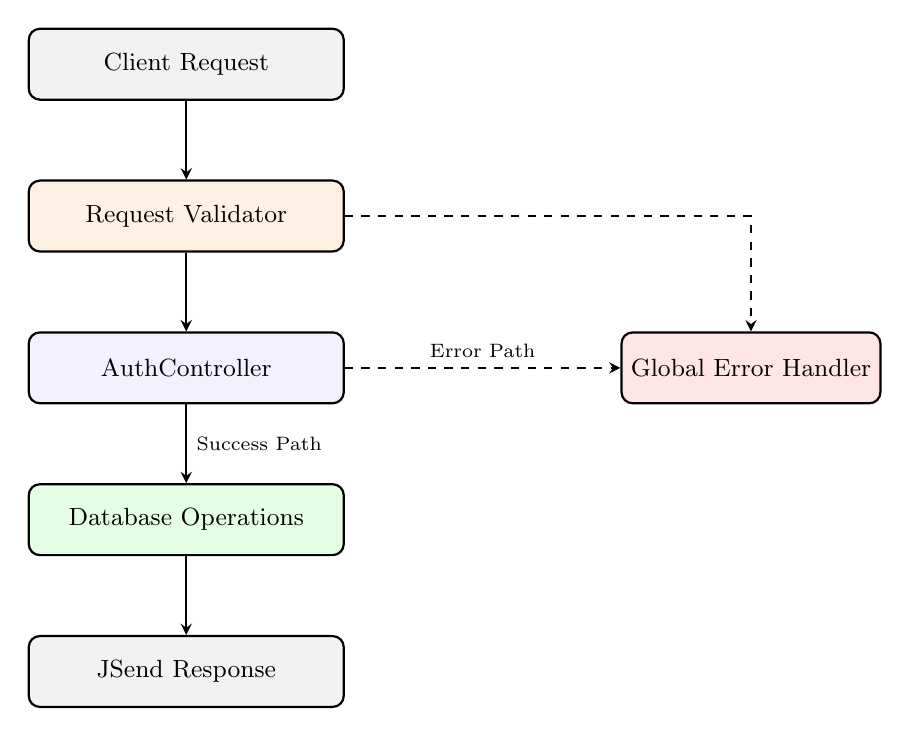
\begin{tikzpicture}[
  node distance=1.0cm and 2.5cm,
  box/.style={rectangle, draw=black, fill=blue!5, thick, minimum width=4cm, minimum height=0.9cm, text centered, rounded corners, font=\small},
  middleware/.style={rectangle, draw=black, fill=orange!10, thick, minimum width=4cm, minimum height=0.9cm, text centered, rounded corners, font=\small},
  logic/.style={rectangle, draw=black, fill=green!10, thick, minimum width=4cm, minimum height=0.9cm, text centered, rounded corners, font=\small},
  err/.style={rectangle, draw=black, fill=red!10, thick, minimum width=3cm, minimum height=0.9cm, text centered, rounded corners, font=\small},
  arrow/.style={thick, ->, >=stealth},
  dashed_arrow/.style={thick, ->, >=stealth, dashed}
]

% Main Flow
\node (client) [box, fill=gray!10] {Client Request};
\node (val) [middleware, below=of client] {Request Validator};
\node (cont) [box, below=of val] {AuthController};
\node (prisma) [logic, below=of cont] {Database Operations};
\node (resp) [box, fill=gray!10, below=of prisma] {JSend Response};

% Error Flow
\node (error) [err, right=of cont, xshift=1cm] {Global Error Handler};

% Arrows
\draw [arrow] (client) -- (val);
\draw [arrow] (val) -- (cont);
\draw [arrow] (cont) -- (prisma) node[midway, right, font=\scriptsize] {Success Path};
\draw [arrow] (prisma) -- (resp);
\draw [dashed_arrow] (cont.east) -- (error.west) node[midway, above, font=\scriptsize] {Error Path};
\draw [dashed_arrow] (val.east) -| (error.north);

\end{tikzpicture}
\caption{End-to-end flow for Registration and Login}
\label{fig:auth-flow}
\end{figure}

\begin{itemize}
    \item \textbf{Registration}: Upon receiving a request, the validator checks the payload. The \texttt{register} controller handles the hashing of passwords/OTPs and executes a transaction to store the user in Prisma. If an existing user is found or database operations fail, the flow routes to the \texttt{Global Error Handler}.
    \item \textbf{Login}: The \texttt{login} controller validates credentials against the database. Upon success, it returns tokens; on failure (e.g., incorrect credentials or disabled account), it throws an \texttt{AppError}, which is caught by the error handler.
\end{itemize}

\subsubsection{Password Reset Flow}
Password recovery utilizes a secure two-stage process to prevent unauthorized access.

\begin{figure}[H]
\centering
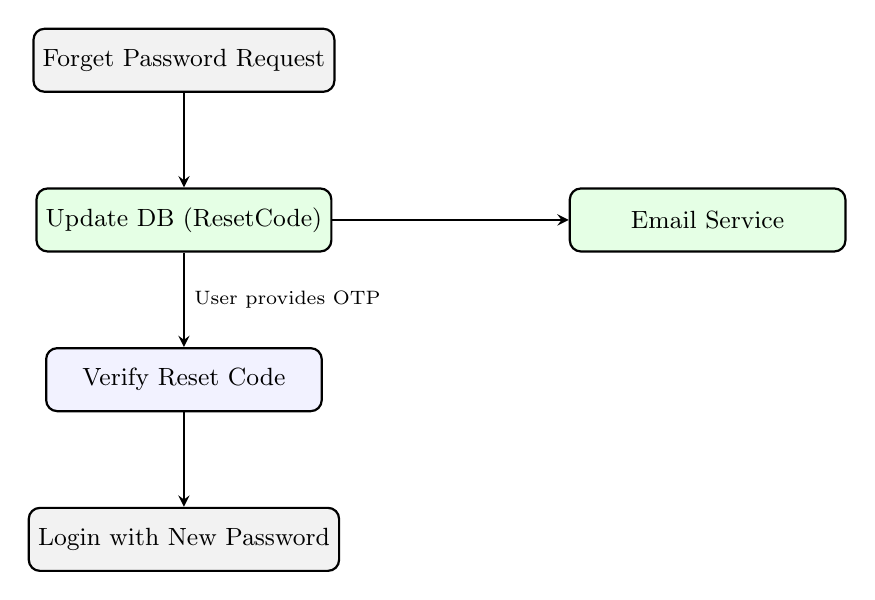
\begin{tikzpicture}[
  node distance=1.2cm and 3cm,
  box/.style={rectangle, draw=black, fill=blue!5, thick, minimum width=3.5cm, minimum height=0.8cm, text centered, rounded corners, font=\small},
  logic/.style={rectangle, draw=black, fill=green!10, thick, minimum width=3.5cm, minimum height=0.8cm, text centered, rounded corners, font=\small},
  arrow/.style={thick, ->, >=stealth}
]

\node (req) [box, fill=gray!10] {Forget Password Request};
\node (db) [logic, below=of req] {Update DB (ResetCode)};
\node (email) [logic, right=of db] {Email Service};
\node (ver) [box, below=of db] {Verify Reset Code};
\node (fin) [box, fill=gray!10, below=of ver] {Login with New Password};

\draw [arrow] (req) -- (db);
\draw [arrow] (db) -- (email);
\draw [arrow] (db) -- (ver) node[midway, right, font=\scriptsize] {User provides OTP};
\draw [arrow] (ver) -- (fin);
\end{tikzpicture}
\caption{Password Reset lifecycle}
\label{fig:reset-flow}
\end{figure}

\begin{enumerate}
    \item \textbf{Initiation}: The \texttt{forgetPassword} controller generates a 15-minute OTP. To prevent user enumeration, it returns a generic success response regardless of the email's validity in the system.
    \item \textbf{Verification}: The \texttt{verifyResetCode} controller hashes the new password and clears the reset code from the database upon success.
\end{enumerate}

\subsubsection{OAuth Authentication Flow}
The OAuth implementation bridges external identity providers and our local application using a ticket-based exchange via Redis.

\begin{figure}[H]
\centering
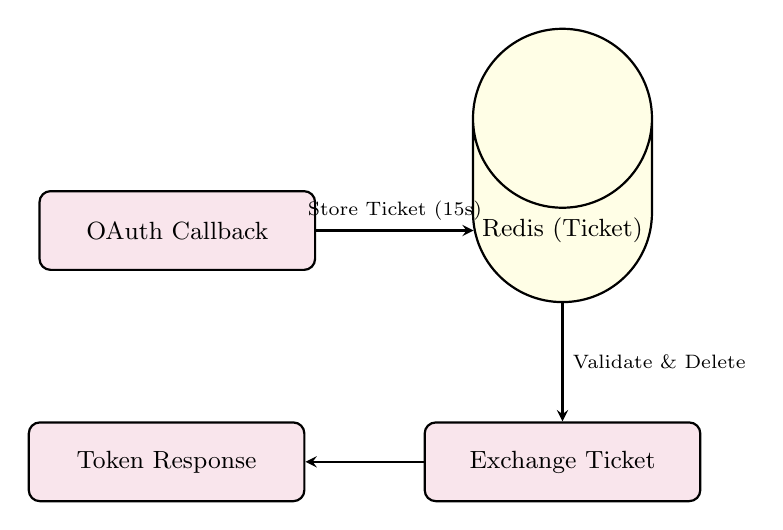
\begin{tikzpicture}[
  node distance=1.5cm,
  process/.style={rectangle, draw=black, fill=purple!10, thick, minimum width=3.5cm, minimum height=1cm, text centered, rounded corners, font=\small},
  storage/.style={cylinder, shape border rotate=90, draw=black, fill=yellow!10, thick, minimum width=1.5cm, minimum height=1cm, text centered, font=\small},
  arrow/.style={thick, ->, >=stealth}
]

\node (auth) [process] {OAuth Callback};
\node (redis) [storage, right=of auth, xshift=0.5cm] {Redis (Ticket)};
\node (ex) [process, below=of redis] {Exchange Ticket};
\node (res) [process, left=of ex] {Token Response};

\draw [arrow] (auth) -- node[above, font=\scriptsize] {Store Ticket (15s)} (redis);
\draw [arrow] (redis) -- node[right, font=\scriptsize] {Validate \& Delete} (ex);
\draw [arrow] (ex) -- (res);
\end{tikzpicture}
\caption{Ticket-based OAuth Exchange mechanism}
\label{fig:oauth-flow}
\end{figure}

\begin{itemize}
    \item \textbf{Callback and Ticket Generation}: Upon successful provider authentication, the callback controller creates a UUID-based "auth ticket" stored in Redis with a 15-second TTL.
    \item \textbf{Exchange}: The client (Web or Flutter) calls the \texttt{exchangeTicket} endpoint with the ticket. The backend validates the ticket against Redis, retrieves the user data, and immediately deletes the ticket to prevent re-use.
\end{itemize}
\subsubsection{User Management Flows}

The user management system focuses on secure profile maintenance and strict data hygiene during account deletion. All user-centric logic is centralized in \texttt{users.controller.ts}.

\paragraph{Profile Update Flow}
The profile update process relies on initial payload validation followed by atomic database updates.

\begin{figure}[H]
\centering
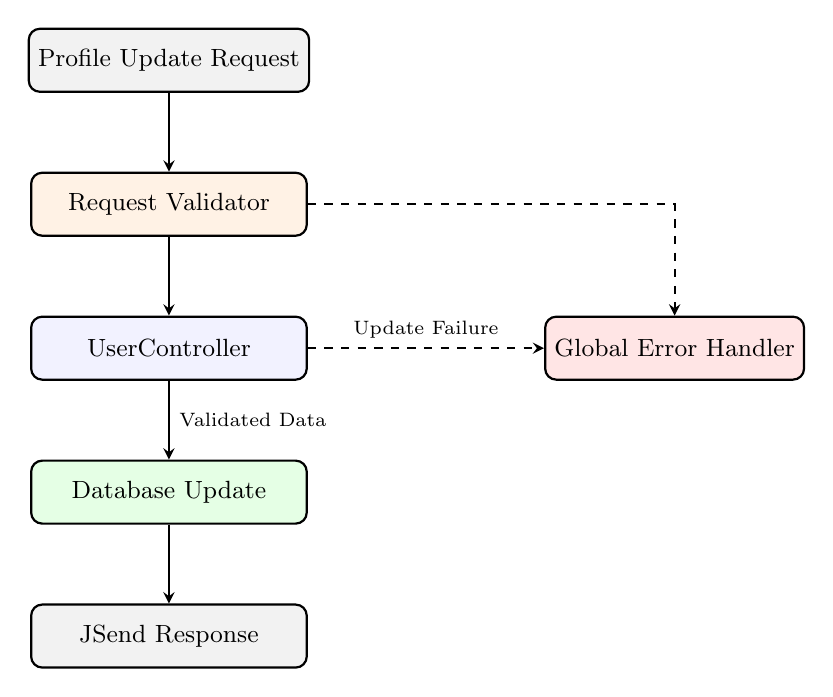
\begin{tikzpicture}[
  node distance=1.0cm and 2.0cm,
  box/.style={rectangle, draw=black, fill=blue!5, thick, minimum width=3.5cm, minimum height=0.8cm, text centered, rounded corners, font=\small},
  middleware/.style={rectangle, draw=black, fill=orange!10, thick, minimum width=3.5cm, minimum height=0.8cm, text centered, rounded corners, font=\small},
  logic/.style={rectangle, draw=black, fill=green!10, thick, minimum width=3.5cm, minimum height=0.8cm, text centered, rounded corners, font=\small},
  err/.style={rectangle, draw=black, fill=red!10, thick, minimum width=3cm, minimum height=0.8cm, text centered, rounded corners, font=\small},
  arrow/.style={thick, ->, >=stealth},
  dashed_arrow/.style={thick, ->, >=stealth, dashed}
]

% Main Flow
\node (client) [box, fill=gray!10] {Profile Update Request};
\node (val) [middleware, below=of client] {Request Validator};
\node (cont) [box, below=of val] {UserController};
\node (prisma) [logic, below=of cont] {Database Update};
\node (resp) [box, fill=gray!10, below=of prisma] {JSend Response};

% Error Flow
\node (error) [err, right=of cont, xshift=1cm] {Global Error Handler};

% Arrows
\draw [arrow] (client) -- (val);
\draw [arrow] (val) -- (cont);
\draw [arrow] (cont) -- (prisma) node[midway, right, font=\scriptsize] {Validated Data};
\draw [arrow] (prisma) -- (resp);
\draw [dashed_arrow] (cont.east) -- (error.west) node[midway, above, font=\scriptsize] {Update Failure};
\draw [dashed_arrow] (val.east) -| (error.north);
\end{tikzpicture}
\caption{End-to-end flow for User Profile Updates}
\label{fig:profile-update-flow}
\end{figure}

\begin{itemize}
    \item \textbf{Orchestration}: Requests are routed through the controller, which verifies user existence and status.
    \item \textbf{Atomic Updates}: Sensitive operations are wrapped in \texttt{prisma.\$transaction} to ensure that data modification and verification status revocation occur simultaneously.
    \item \textbf{Post-Update Logic}: For email changes, the flow triggers the email service and generates fresh security tokens.
\end{itemize}

\paragraph{Account Deletion Flow}
The account deletion process is designed to be comprehensive, ensuring the removal of PII and associated relational assets.

\begin{figure}[H]
\centering
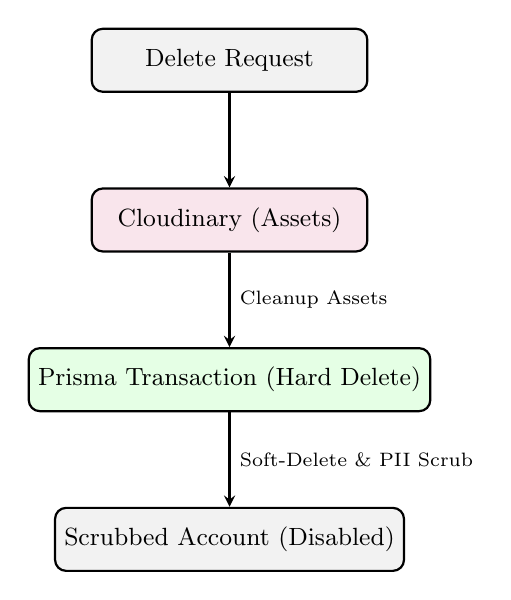
\begin{tikzpicture}[
  node distance=1.2cm and 2.5cm,
  box/.style={rectangle, draw=black, fill=blue!5, thick, minimum width=3.5cm, minimum height=0.8cm, text centered, rounded corners, font=\small},
  logic/.style={rectangle, draw=black, fill=green!10, thick, minimum width=3.5cm, minimum height=0.8cm, text centered, rounded corners, font=\small},
  external/.style={rectangle, draw=black, fill=purple!10, thick, minimum width=3.5cm, minimum height=0.8cm, text centered, rounded corners, font=\small},
  arrow/.style={thick, ->, >=stealth}
]

\node (req) [box, fill=gray!10] {Delete Request};
\node (cloud) [external, below=of req] {Cloudinary (Assets)};
\node (trans) [logic, below=of cloud] {Prisma Transaction (Hard Delete)};
\node (fin) [box, fill=gray!10, below=of trans] {Scrubbed Account (Disabled)};

\draw [arrow] (req) -- (cloud);
\draw [arrow] (cloud) -- (trans) node[midway, right, font=\scriptsize] {Cleanup Assets};
\draw [arrow] (trans) -- (fin) node[midway, right, font=\scriptsize] {Soft-Delete \& PII Scrub};
\end{tikzpicture}
\caption{Account Deletion lifecycle}
\label{fig:deletion-flow}
\end{figure}

\begin{enumerate}
    \item \textbf{Asset Cleanup}: The system invokes Cloudinary to remove user-specific files. This is decoupled from the database transaction.
    \item \textbf{Cascading Hard-Delete}: The system executes multiple \texttt{deleteMany} calls on relational tables (Identity providers, credentials, node inputs, projects).
    \item \textbf{PII Scrubbing}: The user record is disabled, and sensitive information is overwritten with dummy data to satisfy privacy requirements while maintaining referential integrity.
\end{enumerate}

\subsubsection{Project Management Flows}

Project management in the FLOO platform relies on strict access control and centralized request sanitization. All project-related operations are handled by the \texttt{ProjectController}, which enforces data ownership and applies consistent filtering and pagination logic through a helper utility.

\begin{figure}[H]
\centering
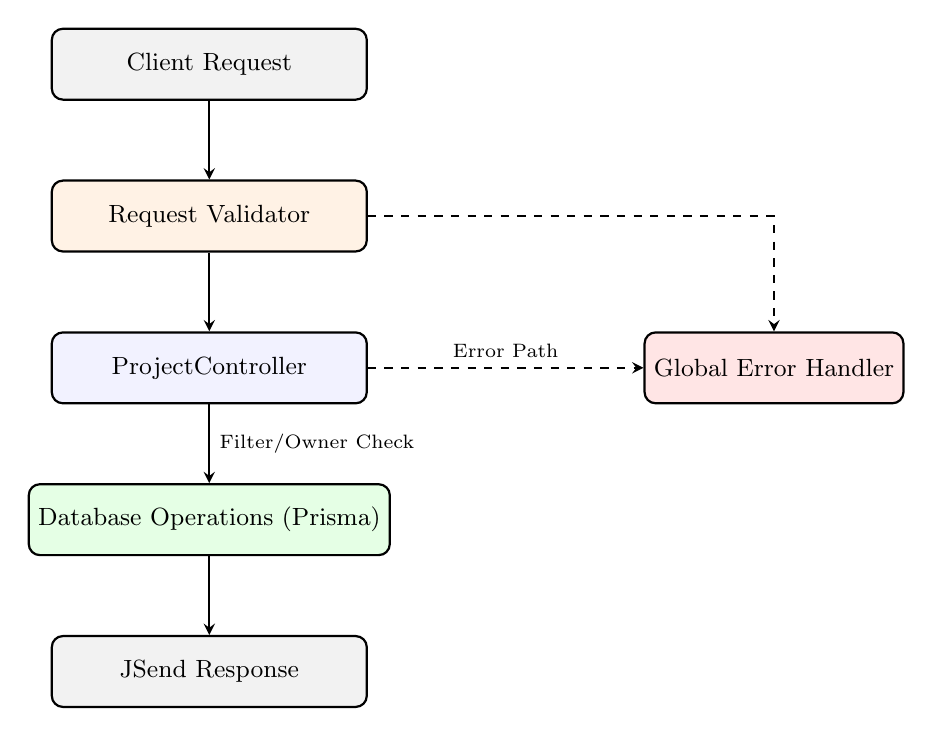
\begin{tikzpicture}[
  node distance=1.0cm and 2.5cm,
  box/.style={rectangle, draw=black, fill=blue!5, thick, minimum width=4cm, minimum height=0.9cm, text centered, rounded corners, font=\small},
  middleware/.style={rectangle, draw=black, fill=orange!10, thick, minimum width=4cm, minimum height=0.9cm, text centered, rounded corners, font=\small},
  logic/.style={rectangle, draw=black, fill=green!10, thick, minimum width=4cm, minimum height=0.9cm, text centered, rounded corners, font=\small},
  err/.style={rectangle, draw=black, fill=red!10, thick, minimum width=3cm, minimum height=0.9cm, text centered, rounded corners, font=\small},
  arrow/.style={thick, ->, >=stealth},
  dashed_arrow/.style={thick, ->, >=stealth, dashed}
]

% Main Flow
\node (client) [box, fill=gray!10] {Client Request};
\node (val) [middleware, below=of client] {Request Validator};
\node (cont) [box, below=of val] {ProjectController};
\node (db) [logic, below=of cont] {Database Operations (Prisma)};
\node (resp) [box, fill=gray!10, below=of db] {JSend Response};

% Error Flow
\node (error) [err, right=of cont, xshift=1cm] {Global Error Handler};

% Arrows
\draw [arrow] (client) -- (val);
\draw [arrow] (val) -- (cont);
\draw [arrow] (cont) -- (db) node[midway, right, font=\scriptsize] {Filter/Owner Check};
\draw [arrow] (db) -- (resp);
\draw [dashed_arrow] (cont.east) -- (error.west) node[midway, above, font=\scriptsize] {Error Path};
\draw [dashed_arrow] (val.east) -| (error.north);
\end{tikzpicture}
\caption{End-to-end flow for Project management operations}
\label{fig:project-flow}
\end{figure}

\begin{itemize}
    \item \textbf{Filtering and Pagination}: All retrieval operations (\texttt{getProjectsByUserId}, \texttt{getAllProjects}, \texttt{getUserProjects}) utilize the \texttt{getProjectFilters} helper. This function parses query parameters into a typed \texttt{Prisma.ProjectWhereInput} object and standardizes \texttt{take} and \texttt{skip} values for pagination, ensuring consistency across all list endpoints.
    \item \textbf{Owner Enforcement}: Operations modifying or retrieving specific resources (\texttt{getProjectById}, \texttt{deleteProject}, \texttt{updateProject}, \texttt{updateWorkflow}) enforce strict ownership by including the authenticated \texttt{userId} in the Prisma \texttt{where} clause. This prevents unauthorized cross-user access at the database level.
    \item \textbf{Workflow Updates}: The \texttt{updateWorkflow} endpoint performs a multi-step update. After verifying project ownership, it updates the project workflow definition and executes a bulk update on the \texttt{NodeInput} table, marking all associated inputs as \texttt{isDraft: false} to finalize the deployment state.
\end{itemize}
\subsubsection{Credential Management Flow}

The credential management system is designed to securely handle sensitive user parameters, ensuring that secret data is encrypted before storage and masked upon retrieval. All credential logic is centralized in the \texttt{credentials.controller.ts}.

\begin{figure}[H]
\centering
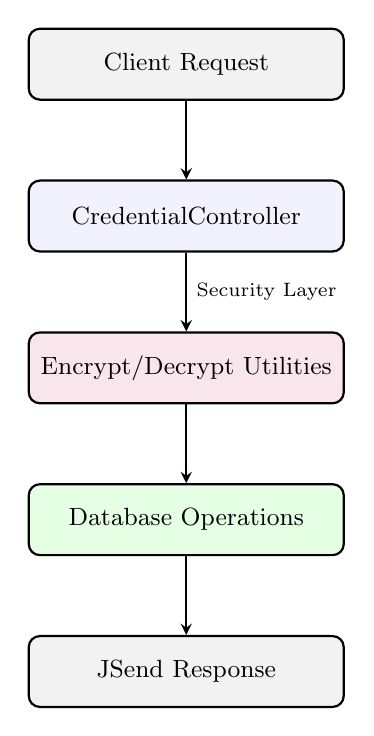
\begin{tikzpicture}[
  node distance=1.0cm and 2.5cm,
  box/.style={rectangle, draw=black, fill=blue!5, thick, minimum width=4cm, minimum height=0.9cm, text centered, rounded corners, font=\small},
  logic/.style={rectangle, draw=black, fill=green!10, thick, minimum width=4cm, minimum height=0.9cm, text centered, rounded corners, font=\small},
  crypto/.style={rectangle, draw=black, fill=purple!10, thick, minimum width=4cm, minimum height=0.9cm, text centered, rounded corners, font=\small},
  arrow/.style={thick, ->, >=stealth}
]

% Main Flow
\node (client) [box, fill=gray!10] {Client Request};
\node (cont) [box, below=of client] {CredentialController};
\node (crypto) [crypto, below=of cont] {Encrypt/Decrypt Utilities};
\node (prisma) [logic, below=of crypto] {Database Operations};
\node (resp) [box, fill=gray!10, below=of prisma] {JSend Response};

% Arrows
\draw [arrow] (client) -- (cont);
\draw [arrow] (cont) -- (crypto) node[midway, right, font=\scriptsize] {Security Layer};
\draw [arrow] (crypto) -- (prisma);
\draw [arrow] (prisma) -- (resp);
\end{tikzpicture}
\caption{End-to-end flow for Credential Management}
\label{fig:cred-flow}
\end{figure}

\begin{itemize}
    \item \textbf{Credential Creation/Update}: Upon receiving a request, the controller coordinates with the \texttt{encrypt()} utility to secure sensitive parameters before performing Prisma transaction operations.
    \item \textbf{Credential Retrieval}: When fetching sets, the controller decrypts sensitive values using \texttt{decrypt()} and applies a \texttt{maskValue()} helper to ensure sensitive data is not exposed in the API response.
    \item \textbf{Data Integrity}: All operations are protected by authentication and verification middlewares to ensure only the owner of the credential set can access or modify it, maintaining strict ownership boundaries.
\end{itemize}
\subsubsection{Workflow Execution Flow}

The workflow execution flow manages the validation, graph construction, and job enqueuing process. It is orchestrated by the \texttt{WorkflowController}, which ensures the project exists and the user is authorized before invoking the core execution service.

\begin{figure}[H]
\centering
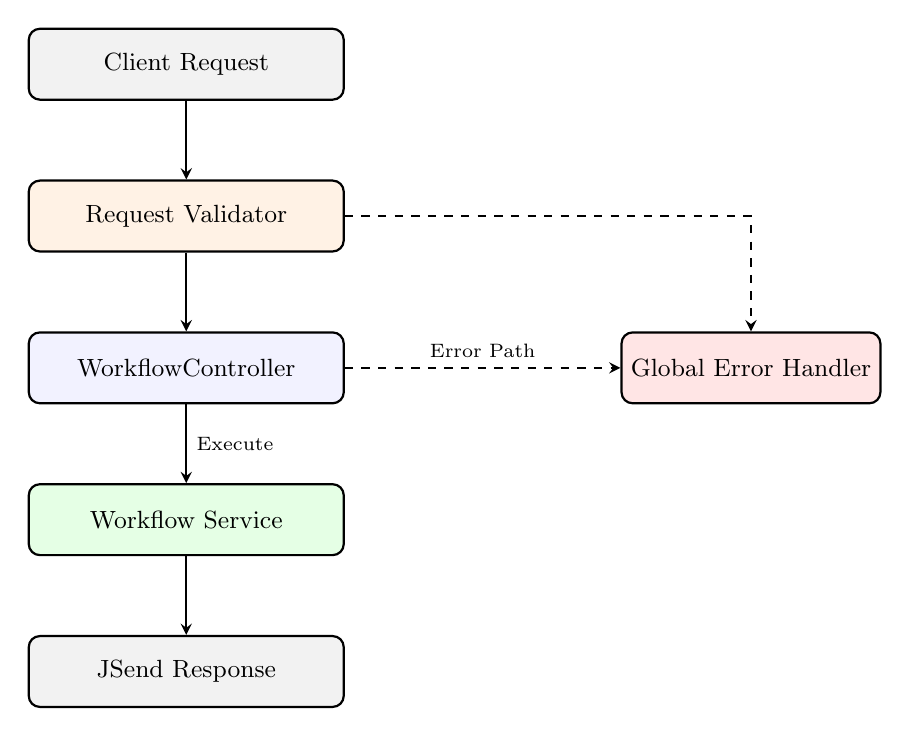
\begin{tikzpicture}[
  node distance=1.0cm and 2.5cm,
  box/.style={rectangle, draw=black, fill=blue!5, thick, minimum width=4cm, minimum height=0.9cm, text centered, rounded corners, font=\small},
  middleware/.style={rectangle, draw=black, fill=orange!10, thick, minimum width=4cm, minimum height=0.9cm, text centered, rounded corners, font=\small},
  logic/.style={rectangle, draw=black, fill=green!10, thick, minimum width=4cm, minimum height=0.9cm, text centered, rounded corners, font=\small},
  err/.style={rectangle, draw=black, fill=red!10, thick, minimum width=3cm, minimum height=0.9cm, text centered, rounded corners, font=\small},
  arrow/.style={thick, ->, >=stealth},
  dashed_arrow/.style={thick, ->, >=stealth, dashed}
]

% Main Flow
\node (client) [box, fill=gray!10] {Client Request};
\node (val) [middleware, below=of client] {Request Validator};
\node (cont) [box, below=of val] {WorkflowController};
\node (service) [logic, below=of cont] {Workflow Service};
\node (resp) [box, fill=gray!10, below=of service] {JSend Response};

% Error Flow
\node (error) [err, right=of cont, xshift=1cm] {Global Error Handler};

% Arrows
\draw [arrow] (client) -- (val);
\draw [arrow] (val) -- (cont);
\draw [arrow] (cont) -- (service) node[midway, right, font=\scriptsize] {Execute};
\draw [arrow] (service) -- (resp);
\draw [dashed_arrow] (cont.east) -- (error.west) node[midway, above, font=\scriptsize] {Error Path};
\draw [dashed_arrow] (val.east) -| (error.north);
\end{tikzpicture}
\caption{End-to-end flow for Workflow Execution}
\label{fig:workflow-execution-flow}
\end{figure}

\begin{itemize}
    \item \textbf{Validation}: Upon receiving the execution request, the controller verifies the presence of the \texttt{projectId} and performs authorization checks against the authenticated user.
    \item \textbf{Service Orchestration}: The controller calls \texttt{executeProjectWorkflow}, which handles the heavy lifting of graph compilation and task scheduling.
    \item \textbf{Error Handling}: Any failure, such as missing IDs or database connectivity issues during the execution setup, throws an \texttt{AppError}, which is caught and formatted by the \texttt{Global Error Handler}.
\end{itemize}

\subsubsection{Node and File Management Flow}

The node and file management flow handles both the retrieval of available system nodes from the registry and the end-to-end lifecycle of files associated with project nodes, including cloud storage uploads and database persistence.

\begin{figure}[H]
\centering
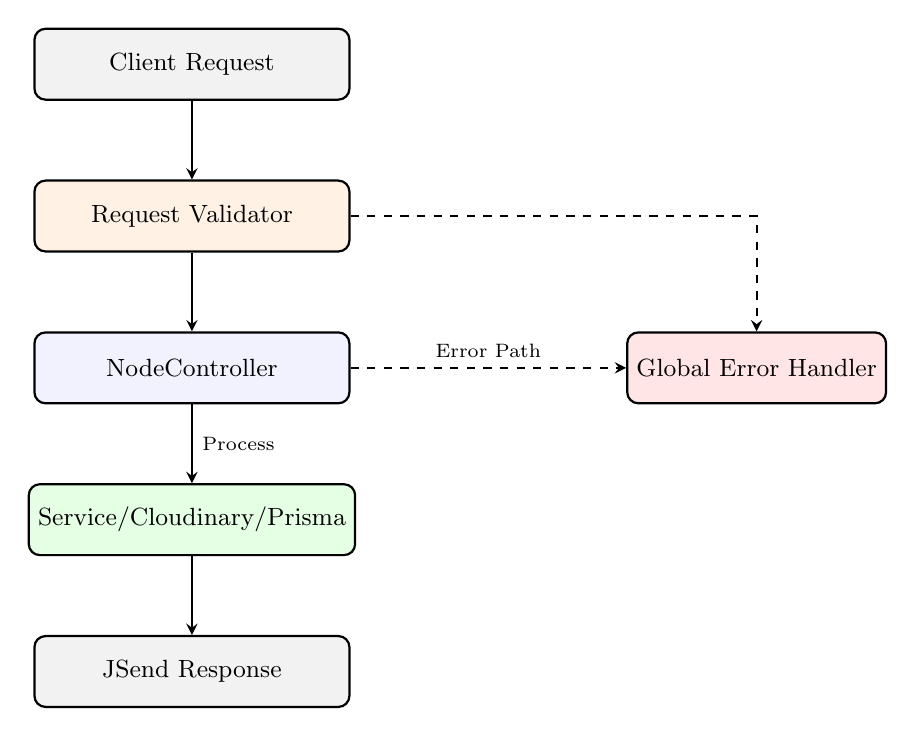
\begin{tikzpicture}[
  node distance=1.0cm and 2.5cm,
  box/.style={rectangle, draw=black, fill=blue!5, thick, minimum width=4cm, minimum height=0.9cm, text centered, rounded corners, font=\small},
  middleware/.style={rectangle, draw=black, fill=orange!10, thick, minimum width=4cm, minimum height=0.9cm, text centered, rounded corners, font=\small},
  logic/.style={rectangle, draw=black, fill=green!10, thick, minimum width=4cm, minimum height=0.9cm, text centered, rounded corners, font=\small},
  err/.style={rectangle, draw=black, fill=red!10, thick, minimum width=3cm, minimum height=0.9cm, text centered, rounded corners, font=\small},
  arrow/.style={thick, ->, >=stealth},
  dashed_arrow/.style={thick, ->, >=stealth, dashed}
]

% Main Flow
\node (client) [box, fill=gray!10] {Client Request};
\node (val) [middleware, below=of client] {Request Validator};
\node (cont) [box, below=of val] {NodeController};
\node (service) [logic, below=of cont] {Service/Cloudinary/Prisma};
\node (resp) [box, fill=gray!10, below=of service] {JSend Response};

% Error Flow
\node (error) [err, right=of cont, xshift=1cm] {Global Error Handler};

% Arrows
\draw [arrow] (client) -- (val);
\draw [arrow] (val) -- (cont);
\draw [arrow] (cont) -- (service) node[midway, right, font=\scriptsize] {Process};
\draw [arrow] (service) -- (resp);
\draw [dashed_arrow] (cont.east) -- (error.west) node[midway, above, font=\scriptsize] {Error Path};
\draw [dashed_arrow] (val.east) -| (error.north);
\end{tikzpicture}
\caption{End-to-end flow for Node and File Operations}
\label{fig:node-management-flow}
\end{figure}

\begin{itemize}
    \item \textbf{Registry Lookups}: For operations such as fetching nodes or categories, the controller directly interacts with the node registry service to provide the requested configuration data.
    \item \textbf{File Operations}: For file-related routes, the controller orchestrates the interaction between the database (Prisma) and cloud storage (Cloudinary). It enforces strict project ownership validation before initiating uploads or deletions.
    \item \textbf{Error Handling}: Any failure—such as file upload exceptions, unauthorized access to a project's node, or missing parameters—is captured by the controller and delegated to the \texttt{Global Error Handler}.
\end{itemize}

\subsubsection{Execution Management Flow}

The execution management flow provides an interface for interacting with workflow logs, aggregated metrics, and administrative oversight. It ensures that users can access logs or delete executions only within the scope of projects they own, while providing administrative endpoints for platform-wide monitoring.

\begin{figure}[H]
\centering
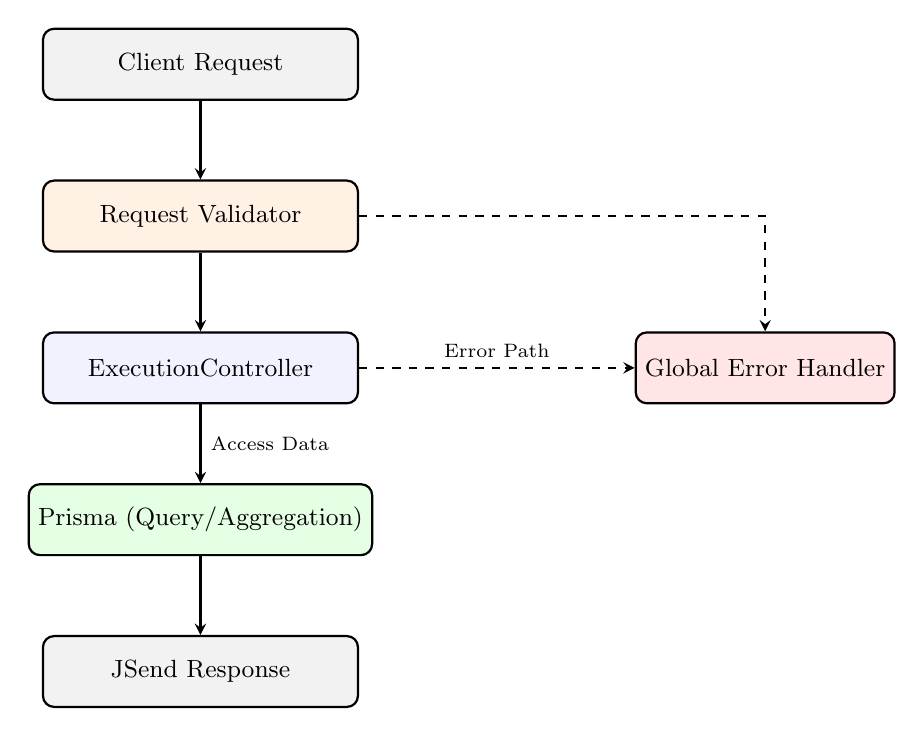
\begin{tikzpicture}[
  node distance=1.0cm and 2.5cm,
  box/.style={rectangle, draw=black, fill=blue!5, thick, minimum width=4cm, minimum height=0.9cm, text centered, rounded corners, font=\small},
  middleware/.style={rectangle, draw=black, fill=orange!10, thick, minimum width=4cm, minimum height=0.9cm, text centered, rounded corners, font=\small},
  logic/.style={rectangle, draw=black, fill=green!10, thick, minimum width=4cm, minimum height=0.9cm, text centered, rounded corners, font=\small},
  err/.style={rectangle, draw=black, fill=red!10, thick, minimum width=3cm, minimum height=0.9cm, text centered, rounded corners, font=\small},
  arrow/.style={thick, ->, >=stealth},
  dashed_arrow/.style={thick, ->, >=stealth, dashed}
]

% Main Flow
\node (client) [box, fill=gray!10] {Client Request};
\node (val) [middleware, below=of client] {Request Validator};
\node (cont) [box, below=of val] {ExecutionController};
\node (db) [logic, below=of cont] {Prisma (Query/Aggregation)};
\node (resp) [box, fill=gray!10, below=of db] {JSend Response};

% Error Flow
\node (error) [err, right=of cont, xshift=1cm] {Global Error Handler};

% Arrows
\draw [arrow] (client) -- (val);
\draw [arrow] (val) -- (cont);
\draw [arrow] (cont) -- (db) node[midway, right, font=\scriptsize] {Access Data};
\draw [arrow] (db) -- (resp);
\draw [dashed_arrow] (cont.east) -- (error.west) node[midway, above, font=\scriptsize] {Error Path};
\draw [dashed_arrow] (val.east) -| (error.north);
\end{tikzpicture}
\caption{End-to-end flow for Execution and Metric Operations}
\label{fig:execution-management-flow}
\end{figure}

\begin{itemize}
    \item \textbf{Data Access and Filtering}: The controller processes incoming requests to retrieve specific executions or aggregated metrics, applying filters for project scope, status, and time range.
    \item \textbf{Security and RBAC}: Each request is validated against the authenticated user's ownership of the project. Administrative routes enforce a role-based access check (RBAC) to ensure only authorized users can delete logs or view platform-wide data.
    \item \textbf{Aggregation Logic}: The \texttt{getUserOverviewMetrics} endpoint leverages Prisma's \texttt{groupBy} functionality to compute success and failure rates dynamically within the database layer, ensuring efficient performance even across high volumes of execution logs.
    \item \textbf{Error Handling}: The controller utilizes centralized error handling for validation failures (e.g., invalid status, project not found) and security violations (e.g., unauthorized deletion attempts).
\end{itemize}

\subsubsection{Webhook Execution Flow}

The webhook execution flow enables external services to programmatically trigger project workflows. Unlike the standard API routes, these endpoints are public and do not require authentication, making them suitable for integrations with third-party platforms. They rely on high-threshold rate limiting to handle spikes in external event traffic while maintaining platform stability.

\begin{figure}[H]
\centering
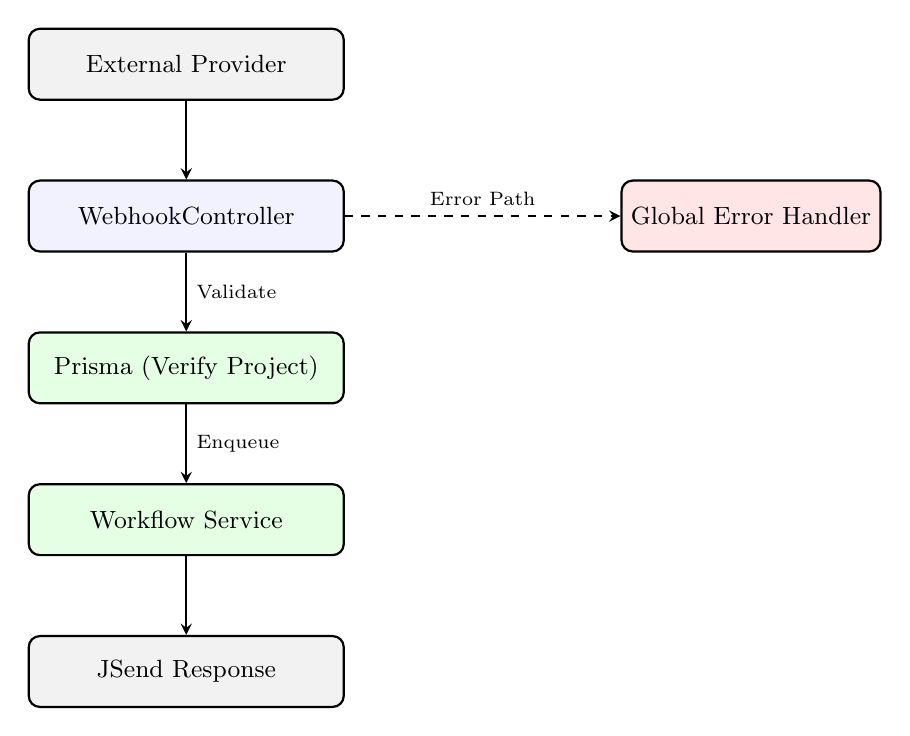
\begin{tikzpicture}[
  node distance=1.0cm and 2.5cm,
  box/.style={rectangle, draw=black, fill=blue!5, thick, minimum width=4cm, minimum height=0.9cm, text centered, rounded corners, font=\small},
  middleware/.style={rectangle, draw=black, fill=orange!10, thick, minimum width=4cm, minimum height=0.9cm, text centered, rounded corners, font=\small},
  logic/.style={rectangle, draw=black, fill=green!10, thick, minimum width=4cm, minimum height=0.9cm, text centered, rounded corners, font=\small},
  err/.style={rectangle, draw=black, fill=red!10, thick, minimum width=3cm, minimum height=0.9cm, text centered, rounded corners, font=\small},
  arrow/.style={thick, ->, >=stealth},
  dashed_arrow/.style={thick, ->, >=stealth, dashed}
]

% Main Flow
\node (client) [box, fill=gray!10] {External Provider};
\node (cont) [box, below=of client] {WebhookController};
\node (db) [logic, below=of cont] {Prisma (Verify Project)};
\node (service) [logic, below=of db] {Workflow Service};
\node (resp) [box, fill=gray!10, below=of service] {JSend Response};

% Error Flow
\node (error) [err, right=of cont, xshift=1cm] {Global Error Handler};

% Arrows
\draw [arrow] (client) -- (cont);
\draw [arrow] (cont) -- (db) node[midway, right, font=\scriptsize] {Validate};
\draw [arrow] (db) -- (service) node[midway, right, font=\scriptsize] {Enqueue};
\draw [arrow] (service) -- (resp);
\draw [dashed_arrow] (cont.east) -- (error.west) node[midway, above, font=\scriptsize] {Error Path};
\end{tikzpicture}
\caption{End-to-end flow for Webhook Workflow Triggers}
\label{fig:webhook-execution-flow}
\end{figure}

\begin{itemize}
    \item \textbf{Verification}: Upon receiving a request, the controller first verifies that the target project exists in the database using Prisma to prevent invalid execution triggers.
    \item \textbf{Execution Trigger}: Once the project is validated, the controller invokes the \texttt{executeProjectWorkflow} service to enqueue the job for processing.
    \item \textbf{Public Accessibility}: These endpoints are designed for high-frequency event sources (e.g., GitHub, Typeform). They bypass standard JWT requirements and are instead protected by specific high-threshold rate limiters to accommodate external spikes without blocking system usage.
    \item \textbf{Error Handling}: The controller handles workflow validation errors and missing project identifiers through the centralized error handling mechanism.
\end{itemize}

\subsubsection{Google Sheets OAuth Controller Flow}

The OAuth controller manages the Google Sheets API authentication callback lifecycle, specifically handling redirects from third-party identity providers. It is responsible for verifying credentials, parsing state information to maintain context (such as the \texttt{projectId}), and securely redirecting the user back to the appropriate frontend interface.

\begin{figure}[H]
\centering
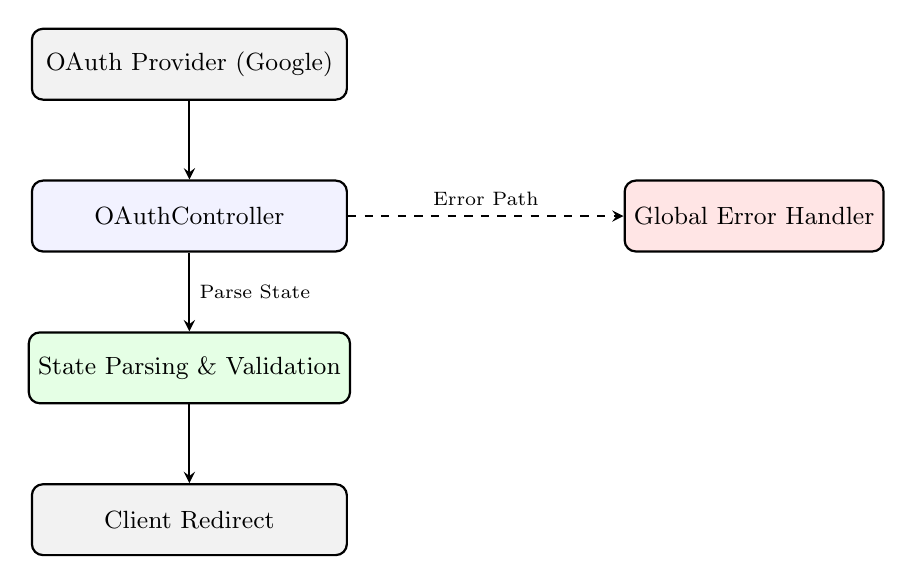
\begin{tikzpicture}[
  node distance=1.0cm and 2.5cm,
  box/.style={rectangle, draw=black, fill=blue!5, thick, minimum width=4cm, minimum height=0.9cm, text centered, rounded corners, font=\small},
  middleware/.style={rectangle, draw=black, fill=orange!10, thick, minimum width=4cm, minimum height=0.9cm, text centered, rounded corners, font=\small},
  logic/.style={rectangle, draw=black, fill=green!10, thick, minimum width=4cm, minimum height=0.9cm, text centered, rounded corners, font=\small},
  err/.style={rectangle, draw=black, fill=red!10, thick, minimum width=3cm, minimum height=0.9cm, text centered, rounded corners, font=\small},
  arrow/.style={thick, ->, >=stealth},
  dashed_arrow/.style={thick, ->, >=stealth, dashed}
]

% Main Flow
\node (client) [box, fill=gray!10] {OAuth Provider (Google)};
\node (cont) [box, below=of client] {OAuthController};
\node (logic) [logic, below=of cont] {State Parsing \& Validation};
\node (resp) [box, fill=gray!10, below=of logic] {Client Redirect};

% Error Flow
\node (error) [err, right=of cont, xshift=1cm] {Global Error Handler};

% Arrows
\draw [arrow] (client) -- (cont);
\draw [arrow] (cont) -- (logic) node[midway, right, font=\scriptsize] {Parse State};
\draw [arrow] (logic) -- (resp);
\draw [dashed_arrow] (cont.east) -- (error.west) node[midway, above, font=\scriptsize] {Error Path};
\end{tikzpicture}
\caption{End-to-end flow for OAuth Callback handling}
\label{fig:oauth-controller-flow}
\end{figure}

\begin{itemize}
    \item \textbf{Credential Verification}: Upon receiving the callback, the controller ensures that the request contains valid user credentials provided by the OAuth strategy.
    \item \textbf{State Parsing}: The controller extracts the \texttt{projectId} from the \texttt{state} query parameter (or request body), enabling the application to resume the workflow context seamlessly.
    \item \textbf{Dynamic Redirection}: Once context is restored, the controller performs a 302 redirect to the frontend workflow canvas, ensuring the user is returned to the exact project they were interacting with.
    \item \textbf{Error Handling}: The controller handles invalid OAuth states or missing identifiers through the centralized error handling mechanism, ensuring failed authentication attempts are caught and reported clearly.
\end{itemize}

\subsection{Middlewares}
\subsubsection{Authentication Middleware}
The \texttt{auth} middleware authenticates requests by verifying the JWT provided in the Authorization header. If the token is missing, it falls back to a query parameter for OAuth redirects. The \texttt{restrictTo} middleware provides fine-grained Role-Based Access Control (RBAC).

\begin{lstlisting}
export const auth = (req: Request, res: Response, next: NextFunction) => {
  try {
    let token = req.headers.authorization;
    if (!token && req.query.token) token = req.query.token as string;
    if (!token) throw new AppError("Unauthorized.", 401);

    const payload = jwt.verify(token, process.env.ACCESS_TOKEN_PRIVATE_KEY!);
    (req as AuthRequest).id = (payload as any).id;
    (req as AuthRequest).role = (payload as any).role;
    next();
  } catch (error) { next(error); }
};

export const restricTo = (...roles: string[]) => {
  return (req: Request, res: Response, next: NextFunction) => {
    if (!roles.includes((req as AuthRequest).role)) 
        return next(new AppError("Forbidden.", 403));
    next();
  };
};
\end{lstlisting}

\subsubsection{Error Handler Middleware}
This middleware acts as a facade for the error registry. It maps caught exceptions to their appropriate handlers based on the \texttt{canHandle} criteria.

\begin{lstlisting}
export const errorHandler = (err: unknown, req: Request, res: Response, next: NextFunction) => {
  const handler = errorHandlerRegistry.find(h => h.canHandle(err));
  if (handler) return handler.handle(err, res);
};
\end{lstlisting}

\subsubsection{Verification Middleware}
The \texttt{restrictToVerified} middleware checks the \texttt{isVerified} status on the request object, ensuring only accounts with confirmed emails can access protected features.

\begin{lstlisting}
export const restrictToVerified = (req: Request, res: Response, next: NextFunction) => {
  if (!(req as AuthRequest).isVerified) {
    throw new AppError("Please verify your email to access this feature.", 403);
  }
  next();
};
\end{lstlisting}

\subsubsection{JSend Middleware}
The \texttt{jsend} middleware standardizes outgoing API responses by attaching helper methods (\texttt{success}, \texttt{fail}, \texttt{error}) to the Express \texttt{Response} object.

\begin{lstlisting}
export function jsend(req: Request, res: Response, next: NextFunction) {
  res.jsend = {
    success: (msg, code = 200, data = null) => 
        res.status(code).json({ status: "success", message: msg, data }),
    fail: (msg, code = 400, data = null) => 
        res.status(code).json({ status: "fail", message: msg, data}),
    error: (msg, code = 500, data = null) => 
        res.status(code).json({ status: "error", message: msg, code, data }),
  };
  next();
}
\end{lstlisting}

\subsubsection{Rate Limiter Middleware}
This factory function generates IP-based rate limiters with configurable time windows and request maximums, throwing a \texttt{429 Too Many Requests} error when limits are exceeded.

\begin{lstlisting}
export const createRateLimiter = (minutes = 15, max = 100, message = "Too many requests.") => {
  return rateLimit({
    windowMs: minutes * 60 * 1000,
    max,
    handler: (req, res, next) => next(new AppError(message, 429)),
  });
};
\end{lstlisting}

\subsubsection{Upload Middleware}
The \texttt{uploadMiddleware} configures \texttt{multer} to handle multipart form data, specifically optimized for file uploads with a 5MB size limit per file.

\begin{lstlisting}
const multerUpload = multer({
  storage: multer.memoryStorage(),
  limits: { fileSize: 5 * 1024 * 1024 },
});

export const uploadMiddleware = (req: Request, res: Response, next: NextFunction) => {
  multerUpload.array("files", 50)(req, res, (err) => {
    if (err instanceof multer.MulterError) return next(new AppError(err.message, 400));
    else if (err) return next(err);
    next();
  });
};
\end{lstlisting}

\subsubsection{Validation Middleware}
The \texttt{validateRequest} middleware executes the results of the \texttt{express-validator} checks. If validation fails, it aggregates the errors and propagates them as a \texttt{422 Unprocessable Entity} exception.

\begin{lstlisting}
export const validateRequest = (req: Request, res: Response, next: NextFunction) => {
  const result = validationResult(req);
  if (!result.isEmpty()) {
    const errors = result.array().map(err => err.msg);
    return next(new AppError('Validation errors', 422, errors));
  }
  next();
};
\end{lstlisting}

\subsection{Validation Layer}

Request validation is abstracted into its own layer using \texttt{express-validator}. Before a request payload is processed, it is checked against strict schemas to ensure data integrity and type safety. This ``fail-fast'' approach guarantees that the underlying controllers and services do not need to perform redundant sanity checks on incoming data .

\subsubsection{Authentication Validators}
These validators enforce security policies for user sessions and account recovery.
\begin{lstlisting}[caption={Authentication validation schemas}]
// auth.validators.ts
export const registerValidators = [
  body('email').notEmpty().withMessage('Empty email').isEmail(),
  body('password').isStrongPassword({ minLength: 8, ... }),
  body('firstName').isLength({ min: 3, max: 15 }),
  body('lastName').isLength({ min: 3, max: 15 })
];

export const loginValidators = [
  body('email').notEmpty().isEmail(),
  body('password').notEmpty()
];

export const verifyEmailValidators = [
  body('email').notEmpty().isEmail(),
  body('code').notEmpty().isNumeric()
];

export const resetCodeValidators = [
  body('email').notEmpty().isEmail(),
  body('resetCode').notEmpty().isNumeric(),
  body('password').notEmpty().isStrongPassword(...)
];
\end{lstlisting}

\subsubsection{Credential Validators}
These ensure that credential definitions maintain proper parameter structures and validation constraints.
\begin{lstlisting}[caption={Credential type validation schema}]
// credential.validator.ts
export const createCredentialTypeValidators = [
  body('title').isLength({ min: 1, max: 100 }),
  body('parameters').isArray({ min: 1 }),
  body('parameters.*.title').isLength({ min: 1, max: 100 }),
  body('parameters.*.maxChar').optional().isInt({ min: 1 }),
  body('parameters.*.isSensitive').optional().isBoolean()
];
\end{lstlisting}

\subsubsection{Project Validators}
Project management routes utilize these validators to constrain metadata and versioning data.
\begin{lstlisting}[caption={Project creation and update validation}]
// project.validators.ts
export const createProjectValidators = [
  body('name').notEmpty().isLength({ min: 1, max: 50 }),
  body('description').optional().isLength({ min: 1, max: 200 }),
  body('type').notEmpty(),
  body('versionId').optional().isNumeric()
];

export const updateProjectValidators = [
  body('name').optional().isLength({ min: 1, max: 50 }),
  body('description').optional().isLength({ min: 1, max: 200 }),
  body('type').optional().isLength({ min: 1 }),
  body('versionId').optional().isNumeric()
];
\end{lstlisting}

\subsubsection{User Validators}
These validators secure user profile modifications, preventing invalid name formats, unauthorized email changes, or weak password updates.
\begin{lstlisting}[caption={User profile and account validation}]
// user.validators.ts
export const updateProfileValidators = [
  body('firstName').optional().isLength({ min: 3, max: 15 }),
  body('lastName').optional().isLength({ min: 3, max: 15 }),
  body('personalizations').optional().isObject()
];

export const updateEmailValidators = [
  body('email').notEmpty().isEmail()
];

export const updatePassword = [
  body('password').notEmpty().isStrongPassword(...)
];
\end{lstlisting}

\subsection{Services}
\subsubsection{Email and Notification Services}

\paragraph{Overview}
The email subsystem is designed to handle automated communications, such as user verification and password reset flows, in a decoupled and highly maintainable manner. It separates the concerns of email configuration, template management, and transport, allowing the application to add new email types or switch transport providers without modifying the core business logic.

\paragraph{Email Service Layer}
The email service layer relies on a modular architecture located in \texttt{backend/src/api/services/email/}, comprising four distinct components that manage the full lifecycle of an outgoing message.

\subparagraph{Email Configuration}
The \texttt{email.config.ts} file serves as a centralized registry for all email types supported by the system. By mapping an \texttt{EmailType} to its specific subject and HTML template, the system ensures consistent messaging and simplifies the addition of new email types.

\begin{lstlisting}[caption={Email configuration registry (\texttt{email.config.ts})}]
export const emailConfig = {
  verify: {
    subject: "Verify your email",
    template: "verify-email",
  },
  reset: {
    subject: "Reset your password",
    template: "reset-password",
  },
};

export type EmailType = keyof typeof emailConfig;
\end{lstlisting}

\subparagraph{Template Loader}
The \texttt{templateLoader.ts} utility abstracts the filesystem operations required to handle HTML templates. It provides two core functions: \texttt{loadTemplate}, which retrieves raw HTML from the \texttt{templates/} directory, and \texttt{renderTemplate}, which performs string interpolation to inject dynamic data (such as OTP codes or user names) into the templates before sending.

\subparagraph{Transporter}
The \texttt{transporter.ts} file encapsulates the initialization of the Nodemailer transport mechanism. By isolating this logic, the system allows for the configuration of various SMTP drivers or API-based mail providers (e.g., SendGrid, Mailgun) in a single location, which the \texttt{email.service.ts} consumes to perform the actual network dispatch.

\subparagraph{Email Service}
The \texttt{email.service.ts} acts as the primary orchestrator for the email subsystem. It exposes a single, clean function, \texttt{sendEmail}, which accepts the email type and dynamic data, looks up the configuration, renders the template, and invokes the transporter.

\begin{lstlisting}[caption={Email service orchestration (\texttt{email.service.ts})}]
export const sendEmail = async (
  type: EmailType,
  to: string,
  data: Record<string, string>
) => {
  // Get the email configuration for the specified type
  const config = emailConfig[type];

  const rawTemplate = loadTemplate(config.template);
  const html = renderTemplate(rawTemplate, data);

  // Send the email using the transporter
  await transporter.sendMail({
    to,
    subject: config.subject,
    html,
  });
};
\end{lstlisting}

\paragraph{SMTP Service}
While the \texttt{email.service.ts} handles templated system emails, the \texttt{smtp.service.ts} (located in \texttt{backend/src/api/services/}) provides a lower-level, credential-based interface for sending arbitrary emails. This is critical for features where users must provide their own SMTP credentials (e.g., connecting a personal Gmail or Outlook account to an automation node).

The service handles the secure retrieval of encrypted SMTP credentials from the database, the construction of a dynamic Nodemailer transporter, and the execution of the mail send process.

\begin{lstlisting}[caption={SMTP execution flow (\texttt{smtp.service.ts})}]
export async function sendEmailSMTP(
  smtpData: SmtpCredentialData,
  emailParams: SmtpEmailParams,
) {
  try {
    const transporter = nodemailer.createTransport({
      host: smtpData.host,
      port: smtpData.port,
      secure: smtpData.secure,
      auth: {
        user: smtpData.username,
        pass: smtpData.password,
      },
    });

    await transporter.sendMail({
      from: smtpData.username,
      to: emailParams.to,
      subject: emailParams.subject,
      text: emailParams.body,
    });

    return { success: true };
  } catch (error: any) {
    throw new AppError(`Failed to send email: ${error.message}`, 500);
  }
}


\end{lstlisting}
\subsubsection{Cloud and AI Services}

\paragraph{Cloudinary Service}
The Cloudinary service acts as the primary storage layer for the platform, handling file uploads and asset management. It leverages Node.js streams to pipe file buffers directly to Cloudinary's infrastructure, ensuring efficient memory usage.

\subparagraph{Uploading Assets}
The \texttt{uploadToCloudinary} function encapsulates the logic for streaming file buffers. By using \texttt{cloudinary.uploader.upload\_stream}, the system avoids loading large files entirely into RAM, which is critical for system stability.

\begin{lstlisting}[caption={Cloudinary upload logic (\texttt{cloudinary.service.ts})}]
export const uploadToCloudinary = async (folder: string, fileBuffer: Buffer): Promise<UploadResult> => {
  return new Promise((resolve, reject) => {
    const stream = cloudinary.uploader.upload_stream(
      {
        folder,
        resource_type: "auto",
        use_filename: true,
        unique_filename: false,
        overwrite: true,
      },
      (error, result) => {
        if (error) {
          reject(new AppError(`Upload failed: ${error.message}`, 500));
        } else {
          resolve({
            url: result!.secure_url,
            publicId: result!.public_id,
          });
        }
      }
    );
    stream.end(fileBuffer);
  });
};
\end{lstlisting}

\subparagraph{Resource Deletion}
Cloudinary requires an explicit \texttt{resource\_type} for deletion (e.g., "image", "video", "raw"). The service includes a helper function, \texttt{toCloudinaryResourceType}, which derives this type from the asset's MIME type to ensure compatibility with Cloudinary's API requirements.

\paragraph{AI and LLM Services}
The AI infrastructure is bifurcated into a lightweight SDK wrapper (\texttt{groq.service.ts}) and a high-level service layer (\texttt{LLMChat.service.ts}) that orchestrates message formatting and prompt execution.

\subparagraph{Groq Integration}
The \texttt{groq.service.ts} initializes the Groq SDK with the required API key from the environment. This serves as a singleton instance used throughout the backend for interacting with LLM models.

\subparagraph{LLMChat Service}
The \texttt{LLMChat.service.ts} provides a simplified, polymorphic interface for the chat completion API. It supports function overloading, allowing developers to generate a reply either from a simple string or from a fully formed array of conversation messages.

\begin{lstlisting}[caption={LLM Chat service with polymorphic input (\texttt{LLMChat.service.ts})}]
// overload signatures
export async function generateReply(messages: Message[]): Promise<string>; 
export async function generateReply(message: string): Promise<string>; 

// implementation
export async function generateReply(input: Message[] | string): Promise<string> {
  const messages: Message[] =
    typeof input === "string"
      ? [{ role: "user", content: input }]
      : input;

  const response = await groq.chat.completions.create({
    model: "openai/gpt-oss-120b", 
    messages,
  });

  return response.choices[0]?.message?.content || "";
}
\end{lstlisting}

This abstraction ensures that the business logic can consume AI responses without needing to handle the complexity of message formatting or model-specific configuration.

\subsubsection{Execution and Node Management Services}

\paragraph{Workflow Service}
The Workflow service is responsible for the orchestration and deployment lifecycle of project workflows. It acts as the bridge between the API controller and the execution engine.

\subparagraph{Workflow Execution Lifecycle}
The \texttt{executeProjectWorkflow} function in \texttt{workflow.service.ts} handles the complete lifecycle of a workflow execution. It performs the following orchestration steps:

\begin{enumerate}
    \item \textbf{Ownership \& State Validation}: Verifies the project existence, authorization, and ensures the project is not already deployed.
    \item \textbf{Graph Construction}: Invokes \texttt{getWorkflowGraph} to compile the raw JSON workflow payload into a structured \texttt{WorkflowGraph} instance.
    \item \textbf{Pre-Execution Validation}: Validates the compiled graph to ensure there are no disconnected nodes or invalid sub-workflows using \texttt{validateAllWorkflows}.
    \item \textbf{Deployment}: Updates the project status in the database and triggers the execution engine via \texttt{enqueueTriggerNodes}.
\end{enumerate}



\paragraph{Node Registry Service}
The Node Registry service, defined in \texttt{nodes.service.ts}, provides a lightweight interface for the frontend to discover available automation nodes.

\subparagraph{Registry Discovery}
The service leverages the \texttt{NodeRegistry} singleton to retrieve all available node classes. It processes these into a consumable format for the frontend UI:

\begin{lstlisting}[caption={Node retrieval logic (\texttt{nodes.service.ts})}]
export const getNodesFromRegistry = () => {
    const registry = NodeRegistry.getInstance();
    const nodes = registry.getAllnodes();
    const nodeDescriptions: any[] = [];
    for (const [key, NodeClass] of nodes) {
      const description = (NodeClass as any).description;
      nodeDescriptions.push({
          ...description,
          url: `https://res.cloudinary.com/dwtdta9o3/image/upload/${description.name}.png`
      });
    }
    return nodeDescriptions;
}
\end{lstlisting}

This approach ensures that the frontend dynamically receives accurate node metadata, including display names, categories, and icon URLs, without hardcoding these values in the client-side application.

\paragraph{Node Output Service}
The Node Output service (\texttt{nodeoutput.service.ts}) manages the storage and persistence of files generated by nodes during execution.

\subparagraph{File Handling and Persistence}
The service enforces strict validation rules—limiting file size to 5MB and a maximum of 50 files per request—before initiating the storage process.

\begin{itemize}
    \item \textbf{Storage}: It iterates through the provided file buffer array and uses the \texttt{uploadToCloudinary} helper to store assets in a structured directory path: \texttt{users/\{userId\}/projects/\{projectId\}/outputs/execution/\{executionId\}/\{nodeId\}}.
    \item \textbf{Database Persistence}: Upon successful cloud upload, the service creates a record in the \texttt{NodeOutput} database table, linking the Cloudinary public ID and secure URL to the specific execution and node context.
\end{itemize}

This atomic orchestration ensures that every file tracked by the database is correctly backed by physical storage, maintaining data integrity for execution logs.

\subsection{Authentication Strategies}

\subsubsection{Overview}
The strategies layer encapsulates interchangeable authentication algorithms and service integrations using the Passport.js framework. This layer acts as the interface between the platform and external identity providers (IdPs) or service APIs, normalizing disparate authentication protocols into a unified internal workflow. By isolating these integrations, the platform can easily scale support for new services without modifying core business logic.

\subsubsection{OAuth Identity Providers}
The system implements three primary OAuth authentication strategies: Discord, GitHub, and Google. While each interacts with a different service provider, they adhere to a consistent internal contract defined by the following execution flow:

\begin{enumerate}
    \item \textbf{Identity Verification}: Upon callback, the strategy queries the \texttt{AuthIdentityProvider} table in the database to determine if the provider-specific ID is already linked to an existing system user.
    \item \textbf{User Upsert}: If no valid identity exists, the logic attempts to match the provider email against existing user records. 
    \begin{itemize}
        \item If a match is found, the strategy updates the existing account to link the new provider ID.
        \item If no match is found, a new user record is created with the default role of 'USER'.
    \end{itemize}
    \item \textbf{Audit Logging}: Every authentication attempt (successful or erroneous) is recorded in the \texttt{AuthHistory} table, which tracks the provider type, status, and error details for security monitoring.
\end{enumerate}

\begin{lstlisting}[caption={Common OAuth identity logic (Discord Strategy)}]
// discord.strategy.ts
const findAuth = await prisma.authIdentityProvider.findUnique({
  where: { provider: "discord", providerId: profile.id },
  include: { user: true },
});

// Update or create user flow
if (!findAuth || findAuth.user.disabled) {
    const existingUser = await prisma.user.findUnique({ 
        where: { email }, 
        include: { authIdentities: true } 
    });
    // Link identity or create new user...
}
\end{lstlisting}

\subsubsection{Google Sheets Integration}
The Google Sheets strategy differs from the standard OAuth providers; it is a service-based strategy rather than an authentication-only strategy. Its primary responsibility is the secure management of third-party API credentials.

\paragraph{Credential Management}
This strategy handles the extraction of tokens during the OAuth callback and manages their persistence using the \texttt{userCredentialSet} and \texttt{userCredentialValue} models.

A critical requirement of this strategy is the security of stored tokens. The strategy explicitly invokes the encryption utility layer before persisting data to the database, ensuring that sensitive access and refresh tokens are never stored in plain text.

\begin{lstlisting}[caption={Credential encryption and storage flow}]
// googleSheet.strategy.ts
const encryptedAccessToken = encrypt(accessTokenValue);
await upsertCredentialValue(
    credentialSet.id, 
    accessTokenParam.id, 
    encryptedAccessToken
);

if (refreshTokenValue && refreshTokenParam) {
  const encryptedRefreshToken = encrypt(refreshTokenValue);
  await upsertCredentialValue(
      credentialSet.id, 
      refreshTokenParam.id, 
      encryptedRefreshToken
  );
}
\end{lstlisting}

This architectural choice separates the concerns of account authentication from resource delegation, allowing the platform to maintain secure, persistent access to external resources like Google Sheets on behalf of the user.
\subsection{Types}
TypeScript interfaces and type definitions form the foundational contract of the application. This layer defines the exact shape of data structures used across the system, ensuring strict compile-time safety and catching structural mismatches between the frontend payloads, the internal API representation, and the execution engine.

\subsubsection{Authentication Request (\texttt{authRequest.type.ts})}
This interface extends the standard Express \texttt{Request} object to inject custom user context. It is used by authentication middlewares to propagate identity information, including the user's unique identifier, role (used for RBAC), email, and their verification status throughout the request lifecycle.

\begin{lstlisting}[caption={Authentication Request Interface}]
import { Request } from 'express';

export interface AuthRequest extends Request {
  id: string;
  role: string;
  email: string;
  isVerified: boolean;
}
\end{lstlisting}

\subsubsection{Google OAuth Profile (\texttt{googleProfile.type.ts})}
This interface standardizes the data structure returned by the Passport.js Google OAuth strategy. It maps the raw profile information into a typed object, allowing the application to securely extract user details like email, name, and locale during the OAuth callback process.

\begin{lstlisting}[caption={Google OAuth Profile Interface}]
import { Profile } from "passport";

export interface GoogleProfile extends Profile {
  _json: {
    sub: string;
    email: string;
    email_verified: boolean;
    name: string;
    given_name: string;
    family_name: string;
    picture: string;
    locale: string;
  };
}
\end{lstlisting}

\subsection{Utils}
The \texttt{utils} directory houses pure, stateless helper functions shared across multiple layers of the application. By centralizing these cryptographic and session-related operations, the platform prevents code duplication and ensures that critical security logic is handled consistently.

\subsubsection{Hashing Utilities (\texttt{hash.util.ts})}
This utility abstracts password and data hashing using \texttt{bcryptjs}. It provides two asynchronous methods: \texttt{hash} to securely salt and hash strings (utilizing environment-configured salt rounds), and \texttt{compareHash} to verify plain-text inputs against existing hashes. This ensures that sensitive credentials are never stored in plaintext.

\begin{lstlisting}[caption={Hashing and Comparison Utility}]
import bcrypt from 'bcryptjs'

const SALT_ROUNDS = Number(process.env.SALT_ROUNDS) || 10;

// Hash value
export const hash = async (value: string) => {
  return await bcrypt.hash(value!, SALT_ROUNDS)
}

// Compare unhashed with hashed value
export const compareHash = async (value: string, hashed: string) => {
  return bcrypt.compare(value, hashed);
};
\end{lstlisting}

\subsubsection{JWT Token Management (\texttt{jwtTokens.util.ts})}
This utility manages the application's authentication lifecycle by signing JSON Web Tokens (JWT). It generates both a short-lived access token (2 hours) and a long-lived refresh token (14 days), both containing essential user metadata (ID, email, role, verification status) protected by environment-specific private keys.

\begin{lstlisting}[caption={Token Generation Utility}]
import jwt from 'jsonwebtoken'

// Function to generate access and refresh tokens for login
export const generateTokens = (userId: string, userEmail: string, userRole: string, isVerified: boolean) => {

  const accessToken = jwt.sign(
    { id: userId, email: userEmail, role: userRole, isVerified },
    process.env.ACCESS_TOKEN_PRIVATE_KEY!,
    { expiresIn: "2h" }
  );

  const refreshToken = jwt.sign(
    { id: userId, email: userEmail, role: userRole, isVerified },
    process.env.REFRESH_TOKEN_PRIVATE_KEY!,
    { expiresIn: "14d" }
  );

  return { accessToken, refreshToken };
}
\end{lstlisting}

\subsubsection{OTP Generation (\texttt{otp.util.ts})}
This utility leverages \texttt{otplib} to handle one-time password (OTP) generation. It is primarily used during account registration, email updates, and password reset flows to generate time-sensitive tokens sent to the user's email, ensuring verification is authenticated and secure.

\begin{lstlisting}[caption={OTP Generation Utility}]
import { authenticator } from "otplib";

export const generateOtp = async () => {
  const secret = authenticator.generateSecret();
  return authenticator.generate(secret);
}
\end{lstlisting}
\section{Error Handling Mechanism}

\subsection{Overview}
The error handling mechanism provides consistent and maintainable error management across all layers of the application. It is built around a registry pattern that decouples error detection and response logic from 
the middleware layer, allowing new error types to be added without modifying any existing code.

\subsection{Core Abstractions}

\subsubsection{The IErrorHandler Interface}
The foundation of the system is the \texttt{IErrorHandler} interface, which defines a unified contract that all error handlers must fulfill:

\begin{itemize}
    \item \texttt{canHandle(err: unknown): boolean} — determines whether this handler is responsible for the given error.
    \item \texttt{handle(err: unknown, res: Response): void} — sends the appropriate HTTP response for the error.
\end{itemize}

The use of \texttt{unknown} as the type for \texttt{err} in both methods ensures that every concrete handler fully honors the interface contract. Type narrowing happens internally inside each handler's \texttt{handle()} method, where the cast is safe because \texttt{canHandle()} has already confirmed the error type.

\subsubsection{The AppError Class}
\texttt{AppError} is a custom error class that extends the native JavaScript \texttt{Error}. It is used throughout the application to represent known, expected failures such as resource not found or unauthorized access. It carries three properties:

\begin{itemize}
    \item \texttt{statusCode} — the HTTP status code for the response.
    \item \texttt{status} — derived automatically as \texttt{fail} for 4xx codes and \texttt{error} for 5xx codes.
    \item \texttt{payload} — optional additional data attached to the response.
\end{itemize}

\subsection{The Handler Registry Pattern}

\subsubsection{Structure}
Each error category is encapsulated in its own self-contained handler class. The system includes the following handlers:

\begin{itemize}
    \item \texttt{PrismaKnownRequestErrorHandler} — handles known Prisma errors identified by error codes such as unique constraint violations (P2002), record not found (P2025), and connection errors (P1001, 
    P1002).
    \item \texttt{PrismaValidationErrorHandler} — handles malformed queries sent to Prisma.
    \item \texttt{PrismaUnknownRequestErrorHandler} — handles unexpected Prisma request failures.
    \item \texttt{PrismaRustPanicErrorHandler} — handles critical Prisma engine panics.
    \item \texttt{PrismaInitializationErrorHandler} — handles database initialization failures, with specific internal logging per failure cause.
    \item \texttt{JwtErrorHandler} — handles JWT errors including invalid signatures, expired tokens, and tokens used before their valid time.
    \item \texttt{BcryptErrorHandler} — handles errors arising from invalid arguments passed to hashing and comparison operations.
    \item \texttt{NodemailerErrorHandler} — handles SMTP connection and authentication errors with specific internal logging per error code.
    \item \texttt{AppErrorHandler} — handles all intentionally thrown \texttt{AppError} instances from application code.
    \item \texttt{UnexpectedErrorHandler} — a catch-all fallback whose \texttt{canHandle()} always returns \texttt{true}. It must always be the last entry in the registry.
\end{itemize}

\subsubsection{The Registry}
The \texttt{errorHandlerRegistry} is an ordered array of handler instances. The middleware iterates through it and delegates to the first handler whose \texttt{canHandle()} returns \texttt{true}. Order is 
significant: specific handlers must precede general ones, and \texttt{UnexpectedErrorHandler} must always be last.

\subsection{The Error Handler Middleware}
The middleware contains no error-type-specific logic. It iterates the registry and delegates entirely:

\begin{lstlisting}
export const errorHandler = (err, req, res, next) => {
  const handler = errorHandlerRegistry.find(h => h.canHandle(err));
  if (handler) return handler.handle(err, res);
};
\end{lstlisting}

\subsection{Extending the System}
Adding support for a new third-party library error requires two steps:

\begin{enumerate}
    \item Implement the \texttt{IErrorHandler} interface in a new handler class, defining \texttt{canHandle()} for detection and \texttt{handle()} for the response. \item Register the new handler in \texttt{errorHandlerRegistry} before \texttt{AppErrorHandler}.
\end{enumerate}

For known, expected application failures such as not found or unauthorized, no new handler is needed. Throwing \texttt{new AppError(message, statusCode)} anywhere in the application is sufficient, as \texttt{AppErrorHandler} handles it automatically.

\subsection{Design Evaluation}
The error handling mechanism offers clear separation of concerns — each handler owns both the detection and response logic for exactly one error category. The middleware is fully decoupled from third-party libraries, 
depending only on the \texttt{IErrorHandler} abstraction. Each handler is independently testable, with unit tests verifying detection and response logic in isolation. Adding a new error type extends the system 
without modifying any existing code.


\section{Workflow Graph Construction and Pre-Execution Validation}
 
Before any workflow can be executed, the system must transform the raw JSON
payload sent by the frontend into a structured, in-memory graph, and then
verify that the graph is semantically correct. This process occurs in two
successive phases: \textit{graph construction} and \textit{pre-execution
validation}. Both phases complete before a single job is enqueued, ensuring
that the execution engine only receives well-formed, executable workflows.
 
\subsection{Data Model}
 
The type system that underpins the entire workflow engine is defined in
\texttt{workflow.type.ts}. Three core interfaces model the graph structure.
 
\textbf{\texttt{INode}} represents a single node in the workflow. Each node
carries all the information required to execute it: its unique identifier, the
node type name used to look it up in the registry, the project and execution
identifiers, an \texttt{inputSource} policy that decides where the node reads
its inputs from, the actual input and output data arrays, typed parameters,
credential references, and the list of its resolved children.
 
\begin{lstlisting}[caption={Core node interface (\texttt{workflow.type.ts})}]
export interface INode {
  id:           string;   // unique node id within the workflow
  type:         string;   // registry key, e.g. "cron", "poll"
  label:        string;   // human-readable display name
  projectId:    string;
  executionId:  string;   // assigned by the worker at runtime
  inputSource:  'self' | 'parent' | 'combined' | 'any';
  inputs:       string[]; // user-provided inputs for this node
  parentOutputs: string[];// outputs received from the upstream node
  parameters:   any[];
  credentials?: { typeId: string; setId: string }[];
  children:     INode[];  // resolved at deployment time
}
\end{lstlisting}
 
\textbf{\texttt{IConnection}} is deliberately minimal, capturing only the
directed edge between two node identifiers:
 
\begin{lstlisting}[caption={Connection and graph interfaces}]
export interface IConnection {
  source: string;
  target: string;
}
 
export interface IWorkflowGraph {
  nodes:       INode[];
  connections: IConnection[];
}
\end{lstlisting}
 
\textbf{\texttt{IWorkflowExecutionContext}} is the object passed from the API
controller to the workflow runner. It bundles the fully constructed graph with
the project identifier so that downstream functions do not need to accept
multiple unrelated arguments:
 
\begin{lstlisting}
export interface IWorkflowExecutionContext {
  workflowGraph: WorkflowGraph;
  projectId:     string;
}
\end{lstlisting}
 
\subsection{The \texttt{WorkflowGraph} Class}
 
The \texttt{WorkflowGraph} class wraps an \texttt{IWorkflowGraph} value
object with an \textit{adjacency list} for efficient traversal, and exposes
graph operations used by both the validation and execution layers.
 
\subsubsection{Internal Representation}
 
The class maintains two parallel data structures:
 
\begin{itemize}
  \item \texttt{graph} --- the plain \texttt{IWorkflowGraph} object, which
        stores the canonical lists of nodes and connections and is used
        wherever a serialisable snapshot of the graph is needed.
  \item \texttt{adjList} --- a \texttt{Map<string, string[]>} that maps each
        node identifier to the identifiers of its direct successors. This is
        kept in sync with \texttt{graph.connections} whenever
        \texttt{addConnection} is called, allowing $O(1)$ neighbour lookup
        during traversal instead of scanning the full connection list each time.
\end{itemize}
 
\begin{lstlisting}[caption={WorkflowGraph construction (\texttt{workflowGraph.class.ts})}]
export class WorkflowGraph {
  graph:           IWorkflowGraph;
  private adjList: Map<string, string[]>;
 
  constructor() {
    this.graph   = { nodes: [], connections: [] };
    this.adjList = new Map();
  }
 
  addNode(node: INode): void {
    if (this.hasNode(node))
      throw new AppError(`Node with ID ${node.id} already exists`, 400);
    this.graph.nodes.push(node);
  }
 
  addConnection(edge: IConnection): void {
    if (this.hasConnection(edge))
      throw new AppError(
        `Edge from ${edge.source} to ${edge.target} already exists`, 400);
 
    this.graph.connections.push(edge);
 
    if (!this.adjList.has(edge.source))
      this.adjList.set(edge.source, []);
    this.adjList.get(edge.source)!.push(edge.target);
  }
}
\end{lstlisting}
 
Both \texttt{addNode} and \texttt{addConnection} perform a duplicate check
before mutating state, throwing an \texttt{AppError} if the node or edge is
already present. This prevents malformed workflow payloads from producing
silent inconsistencies in the graph.
 
\subsubsection{Finding Trigger Nodes}
 
A trigger node is structurally defined as a node with no incoming edges ---
it sits at the root of a connected component. \texttt{findTriggerNodes}
identifies these nodes using an in-degree approach:
 
\begin{lstlisting}[caption={Trigger node detection by in-degree}]
findTriggerNodes(): INode[] {
  const allIDs      = this.getNodes().map(n => n.id);
  const hasIncoming = new Set<string>();
 
  // collect every node that appears as a target of some edge
  for (const node of this.getNodes())
    this.getNodeConnections(node.id).forEach(n => hasIncoming.add(n));
 
  // nodes absent from hasIncoming have no parents -> they are triggers
  const triggerIDs = allIDs.filter(id => !hasIncoming.has(id));
  return this.graph.nodes.filter(n => triggerIDs.includes(n.id));
}
\end{lstlisting}
 
The method builds the set of all nodes that appear as an edge target. Any
node \textit{not} in that set has an in-degree of zero and is therefore a
candidate trigger. The subsequent validation step then confirms, via the node
registry, that each such candidate is actually declared as a trigger node type.
 
\subsubsection{Decomposing into Connected Components}
 
A workflow canvas may contain multiple independent sub-workflows. Rather than
validating and executing the entire graph as one unit, the system first
decomposes it into \textit{connected components} so that each sub-workflow can
be validated and reported on individually. The decomposition uses BFS over the
\textit{undirected} version of the graph (edges are traversed in both
directions):
 
\begin{lstlisting}[caption={Connected component decomposition (BFS)}]
findConnectedComponents(): WorkflowGraph[] {
  const visited           = new Set<string>();
  const components: WorkflowGraph[] = [];
  const nodeMap           = new Map(this.graph.nodes.map(n => [n.id, n]));
  const reverseConnections = new Map<string, string[]>();
 
  // build a reverse adjacency map to traverse edges backwards
  for (const conn of this.graph.connections) {
    if (!reverseConnections.has(conn.target))
      reverseConnections.set(conn.target, []);
    reverseConnections.get(conn.target)!.push(conn.source);
  }
 
  for (const startNode of this.graph.nodes) {
    if (visited.has(startNode.id)) continue;
 
    const componentGraph = new WorkflowGraph();
    const queue          = [startNode];
    visited.add(startNode.id);
    componentGraph.addNode(startNode);
 
    while (queue.length > 0) {
      const current     = queue.shift()!;
      const forward     = this.adjList.get(current.id)  || [];
      const backward    = reverseConnections.get(current.id) || [];
      const neighbours  = [...new Set([...forward, ...backward])];
 
      for (const nId of neighbours) {
        if (!visited.has(nId)) {
          visited.add(nId);
          componentGraph.addNode(nodeMap.get(nId)!);
          queue.push(nodeMap.get(nId)!);
        }
      }
    }
 
    // copy only the edges that belong to this component
    for (const conn of this.graph.connections)
      if (componentGraph.hasNode({ id: conn.source } as INode) &&
          componentGraph.hasNode({ id: conn.target } as INode))
        componentGraph.addConnection(conn);
 
    components.push(componentGraph);
  }
 
  return components;
}
\end{lstlisting}
 
Treating the graph as undirected during decomposition is important. A directed
BFS from a trigger node would miss any nodes upstream of a cycle or any
disjoint nodes that happen to feed into the same component via reverse edges.
Using both the forward adjacency list and the reverse map guarantees that every
node is assigned to exactly one component regardless of edge direction.
 
\subsection{Graph Construction from the HTTP Request}
 
The \texttt{getWorkflowGraph} function in
\texttt{workflow-pre-execution.validations.ts} is the entry point for turning
a raw request payload into a typed \texttt{WorkflowGraph} instance. It is
called by the workflow controller immediately after the project record is
fetched from the database.
 
\subsubsection{Input Format}
 
The frontend serialises the workflow canvas as a JSON object containing a
\texttt{nodes} array and a \texttt{connections} array. Each node object
follows the React Flow schema, where the node's semantic type is stored inside
a nested \texttt{data.nodeName} field rather than at the top level:
 
\begin{lstlisting}[caption={Example workflow payload from the frontend}]
{
  "projectId": "abc-123",
  "nodes": [
    {
      "id": "cron-1761747201552",
      "data": { "nodeName": "cron", "label": "Scheduled Trigger" },
      "parameters": [
        { "title": "interval", "value": 60000 },
        { "title": "start",    "value": 1700000000000 }
      ],
      "credentials": []
    },
    {
      "id": "sheet-1761747208825",
      "data": { "nodeName": "googleSheet", "label": "Append to Sheet" },
      "parameters": [...],
      "credentials": [{ "typeId": "cb7c448b-...", "setId": "f3a1..." }]
    }
  ],
  "connections": [
    { "source": "cron-1761747201552",
      "target": "sheet-1761747208825", "type": "custom-edge" }
  ]
}
\end{lstlisting}
 
\subsubsection{Parsing and Validation}
 
The function first validates the shape of the incoming data, then maps each
raw node object to a typed \texttt{INode}, and finally populates the graph:
 
\begin{lstlisting}[caption={Graph construction from request body}]
export const getWorkflowGraph =
    (body: Record<string, unknown>): WorkflowGraph => {
 
  // --- shape checks -----------------------------------------------
  const nodesRaw = (body as any).nodes;
  if (!Array.isArray(nodesRaw) ||
      nodesRaw.some(n => typeof n.id !== 'string'))
    throw new AppError('Invalid or missing nodes', 400);
 
  const connectionsRaw = (body as any).connections;
  if (!Array.isArray(connectionsRaw))
    throw new AppError('Invalid or missing connections', 400);
 
  const isValidConnections = connectionsRaw.every(conn =>
    typeof conn.source === 'string' &&
    typeof conn.target === 'string' &&
    typeof conn.type   === 'string'
  );
  if (!isValidConnections)
    throw new AppError('Invalid connections', 400);
 
  // --- mapping -------------------------------------------------------
  const nodes: INode[] = nodesRaw.map(n => ({
    id:           n.id,
    type:         n.data?.nodeName,     // unwrap from React Flow schema
    label:        n.data?.label ?? '',
    projectId:    body.projectId as string,
    executionId:  '',                   // assigned later by the worker
    inputSource:  n.inputSource ?? 'parent',
    inputs:       n.inputs,
    parentOutputs: [],
    parameters:   n.parameters  ?? [],
    credentials:  n.credentials ?? [],
    children:     [],                   // resolved at deployment time
  }));
 
  const connections: IConnection[] = connectionsRaw.map(conn => ({
    source: conn.source,
    target: conn.target,
  }));
 
  // --- graph population ----------------------------------------------
  const graph = new WorkflowGraph();
  nodes.forEach(n => graph.addNode(n));
  connections.forEach(c =>
    graph.addConnection({ source: c.source, target: c.target }));
 
  return graph;
};
\end{lstlisting}
 
Two design details are worth noting. First, \texttt{executionId} is
intentionally left empty at this stage. The worker assigns it later when it
creates the \texttt{Execution} database record, and then propagates it through
all child jobs. Second, \texttt{children} is left as an empty array; the
workflow runner populates it recursively at deployment time via
\texttt{buildChildren}, so that the full execution tree travels with each job
without requiring further graph lookups.
 
\subsection{Pre-Execution Validation Pipeline}
 
Validation is orchestrated by \texttt{validateAllWorkflows}, which runs each
connected component through a sequence of checks. The function returns a
result object that separates valid sub-workflows from invalid ones, along with
the specific error messages for each failure:
 
\begin{lstlisting}[caption={Validation orchestrator}]
export const validateAllWorkflows =
    async (workflowGraph: WorkflowGraph) => {
 
  const validationResults = {
    validWorkflows:   [] as IWorkflowGraph[],
    invalidWorkflows: [] as { workflow: IWorkflowGraph;
                              errors: string[] }[],
  };
 
  const components = workflowGraph.findConnectedComponents();
 
  for (const component of components) {
    const errors: string[] = [];
 
    const unregisteredNodes = checkAllNodesValidation(component);
    const triggerResult     = validateTriggerNodes(component);
 
    if (!triggerResult.ok)
      errors.push(triggerResult.msg!);
 
    if (unregisteredNodes.length > 0) {
      errors.push(`The following nodes are not registered: ` +
        unregisteredNodes
          .map(n => `${n.name} (id: ${n.id})`).join(', '));
 
    } else if (triggerResult.ok && unregisteredNodes.length === 0) {
      // cycle check only runs when the graph structure is already valid
      const cycleResult = checkCycles(component);
      if (!cycleResult.ok)
        errors.push(cycleResult.msg!);
    }
 
    if (errors.length > 0)
      validationResults.invalidWorkflows.push(
        { workflow: component.graph, errors });
    else
      validationResults.validWorkflows.push(component.graph);
  }
 
  return validationResults;
};
\end{lstlisting}
 
The three validators are applied in a deliberate order, described in the
following subsections.
 
\subsubsection{Trigger Node Validation}
 
\texttt{validateTriggerNodes} enforces three structural rules:
 
\begin{enumerate}
  \item The component must contain at least one node.
  \item Every node with no incoming edges (as identified by
        \texttt{findTriggerNodes}) must be declared as a trigger node in the
        registry (\texttt{triggerNode: true}).
  \item No node with incoming edges may be a trigger node --- trigger nodes
        are only valid at the root of a component.
\end{enumerate}
 
\begin{lstlisting}[caption={Trigger node structural validation}]
const validateTriggerNodes =
    (graph: WorkflowGraph): { ok: boolean; msg?: string } => {
 
  const triggerNodes = graph.findTriggerNodes();
 
  if (graph.getNodes().length === 0)
    return { ok: false, msg: 'No nodes found to execute.' };
 
  if (triggerNodes.length === 0)
    return { ok: false, msg: 'No start node found or cycle exists.' };
 
  // every root must be a registered trigger
  for (const node of triggerNodes) {
    const desc = registry.getDescription(node.type);  // throws if unregistered
    if (!desc.triggerNode)
      return { ok: false,
        msg: `Node '${node.type}' (id: '${node.id}') is at the ` +
             `start of the workflow but is not a trigger node.` };
  }
 
  // no non-root node may be a trigger
  for (const node of graph.getNodes()) {
    if (triggerNodes.includes(node)) continue;
    const desc = registry.getDescription(node.type);
    if (desc.triggerNode)
      return { ok: false,
        msg: `Trigger node '${node.type}' (id: '${node.id}') ` +
             `cannot be used in the middle of a workflow.` };
  }
 
  return { ok: true };
};
\end{lstlisting}
 
\subsubsection{Node Registry Validation}
 
\texttt{checkAllNodesValidation} ensures that every non-trigger node in the
component is registered in the \texttt{NodeRegistry}. Trigger nodes are
excluded from this check because their registration is already verified by
\texttt{validateTriggerNodes}.
 
\begin{lstlisting}[caption={Registry membership check for non-trigger nodes}]
const checkAllNodesValidation =
    (workflowGraph: WorkflowGraph): { name: string; id: string }[] => {
 
  const triggerNodeIds = new Set(
    workflowGraph.findTriggerNodes().map(n => n.id));
  const unregistered: { name: string; id: string }[] = [];
 
  for (const node of workflowGraph.graph.nodes) {
    if (triggerNodeIds.has(node.id)) continue;  // skip triggers
    if (!registry.has(node.type))
      unregistered.push({ name: node.type, id: node.id });
  }
 
  return unregistered;
};
\end{lstlisting}
 
If any unregistered nodes are found, their names and identifiers are collected
and returned as a list, which the orchestrator formats into a single error
message. This allows the user to see all unregistered nodes in one response
rather than having to fix them one by one.
 
\subsubsection{Cycle Detection}
 
The cycle check is the last to run and only executes if both preceding checks
pass. This ordering is intentional: running a DFS-based cycle detector on a
graph that contains unregistered nodes or a missing trigger would produce
unreliable or misleading results, since the graph structure cannot be trusted.
 
Cycle detection uses a standard three-colour DFS algorithm, encoded by the
\texttt{VisitState} enum:
 
\begin{lstlisting}[caption={\texttt{VisitState} enum (\texttt{workflow.enum.ts})}]
export enum VisitState {
  UNVISITED = 0,  // not yet reached
  VISITING  = 1,  // currently on the DFS call stack
  VISITED   = 2,  // fully processed, no cycle through this node
}
\end{lstlisting}
 
\begin{lstlisting}[caption={DFS cycle detection}]
const checkCycles =
    (graph: WorkflowGraph): { ok: boolean; msg?: string } => {
 
  const visited = new Map<string, VisitState>(
    graph.getNodes().map(n => [n.id, VisitState.UNVISITED]));
 
  const dfs = (u: string): boolean => {
    visited.set(u, VisitState.VISITING);
 
    for (const v of graph.getNodeConnections(u)) {
      if (visited.get(v) === VisitState.VISITING) return true;  // back edge
      if (visited.get(v) === VisitState.UNVISITED && dfs(v))   return true;
    }
 
    visited.set(u, VisitState.VISITED);
    return false;
  };
 
  for (const node of graph.getNodes())
    if (visited.get(node.id) === VisitState.UNVISITED)
      if (dfs(node.id))
        return { ok: false, msg: 'Workflow has cycles' };
 
  return { ok: true };
};
\end{lstlisting}
 
A node in the \texttt{VISITING} state is one that is currently on the
recursive call stack. Encountering such a node while traversing its own
descendants means a back edge has been found, which is the defining
characteristic of a cycle in a directed graph. Once all descendants of a node
have been processed without finding a back edge, the node is marked
\texttt{VISITED} and will not be re-explored. The outer loop ensures that all
disconnected components --- if \texttt{findConnectedComponents} was bypassed
--- are also checked.
 
\subsection{Validation Ordering and Error Accumulation}
 
The order in which the three validators run is not arbitrary. Table
\ref{tab:validation-order} summarises the rationale for their sequence.
 
\begin{table}[h!]
\centering
\begin{tabular}{clp{7.5cm}}
  \toprule
  \textbf{Order} & \textbf{Validator} & \textbf{Rationale} \\
  \midrule
  1 & \texttt{validateTriggerNodes}   &
      Structural check. A component without a valid trigger root cannot be
      executed at all, and a trigger node in the middle of a graph is a
      logical error that makes the remaining checks meaningless. \\[6pt]
  2 & \texttt{checkAllNodesValidation} &
      Registry check. An unregistered node would cause the worker to throw at
      runtime. Catching this statically produces a clearer error and avoids
      wasting a job queue slot. \\[6pt]
  3 & \texttt{checkCycles} &
      Graph-theoretic check. Only runs when the graph is structurally sound.
      A cyclic graph would cause \texttt{buildChildren} to recurse infinitely
      and flood the job queue, so cycles must be rejected before deployment. \\
  \bottomrule
\end{tabular}
\caption{Pre-execution validation order and rationale}
\label{tab:validation-order}
\end{table}
 
Errors from the trigger and registry checks are accumulated independently and
both reported if both fail. The cycle check is \textit{gated} behind the
registry check: it only executes if all non-trigger nodes are registered, since
a DFS over a graph that references unknown node types cannot be trusted to
reflect the true structure of the intended workflow.
 
Once the full validation result is returned to the workflow controller, any
component listed in \texttt{invalidWorkflows} causes the entire deployment
request to be rejected with a structured error payload identifying the
problematic nodes and the reasons for failure.
 




\marginpar[Margin note.]{Margin par.}


%%%%%%%%%%%%%%%%%%%%%%%%%%%%%%%%%%%%%%%%%%%%%%%%%%%%%%%%%%%%%%%%%%%%%%%%%%%%%%%%
%% Bibliography:
%%
\cleardoublepage
\phantomsection
\addcontentsline{toc}{chapter}{Bibliography}
\bibliographystyle{plainnat}
\bibliography{thesis}



%%%%%%%%%%%%%%%%%%%%%%%%%%%%%%%%%%%%%%%%%%%%%%%%%%%%%%%%%%%%%%%%%%%%%%%%%%%%%%%%
%% Appendix:
%%

\appendix

\chapter{Extra Information}
Some more text ...



%%%%%%%%%%%%%%%%%%%%%%%%%%%%%%%%%%%%%%%%%%%%%%%%%%%%%%%%%%%%%%%%%%%%%%%%%%%%%%%%
%% Index:
%%
\printthesisindex

\end{document}
